\documentclass{article}
\usepackage{mathptmx} % Times font with math support
\usepackage[12pt]{extsizes} % Set the font size to 12pt
\usepackage[margin=1in]{geometry}
\usepackage{graphicx}  % For inserting images
\usepackage{amsmath} % Required for align and other formatting option
\usepackage{float}     % For controlling figure placement
\usepackage{caption}   % For additional captioning options
\usepackage{setspace}  % For spacing control

\doublespacing % Double spacing for the entire document

% \captionsetup[type=figure]{labelsep=period}  % Changes the label separator to a period for figures
% Set captions for figures to single spacing with a period separator
\captionsetup[type=figure]{labelsep=period, font={small, singlespacing}}

% Set captions for tables to single spacing with a period separator
\captionsetup[type=table]{labelsep=period, font={small, singlespacing}}

\usepackage{capt-of}   % For handling captions outside figure environments

% Create a new counter for supplementary figures
\newcounter{suppfig}
\renewcommand{\thesuppfig}{S\arabic{suppfig}}  % Define the numbering as S1, S2, ...

% Redefine the figure environment for supplementary figures
\newenvironment{suppfigure}[1][htbp]
  {\refstepcounter{suppfig}%
   \begin{figure}[#1]%
   \renewcommand{\thefigure}{\thesuppfig}}% Use the supplementary figure numbering as "Figure S1"
  {\end{figure}}

\usepackage[colorlinks=true, linkcolor=blue, urlcolor=blue, citecolor=blue]{hyperref}

\usepackage{ragged2e}






\begin{document}
\title{DECIPHERING RODENT BEHAVIOR: UNRAVELING COMPLEX DECISION-MAKING THROUGH HIGH-THROUGHPUT DATA ANALYSIS IN BEHAVIORAL NEUROSCIENCE}
% Roman page numbering for front matter
\pagenumbering{roman}
\setcounter{page}{1}  % Reset page counter

\thispagestyle{empty}
{\centering 
DECIPHERING RODENT BEHAVIOR: UNRAVELING\\ 
COMPLEX DECISION-MAKING THROUGH\\
HIGH-THROUGHPUT DATA ANALYSIS IN BEHAVIORAL \\
NEUROSCIENCE\\
\vspace{4em}
ATANU GIRI\\
\vspace{1em}
Doctoral Program in Computational Science\\}
\vspace{4em}
\hspace*{0.5\linewidth}APPROVED:
\vspace{4em}
\hspace*{0.5\linewidth}\rule{0.5\linewidth}{0.5mm}\\
\hspace*{0.5\linewidth}Alexander Friedman, Ph.D., Chair\\
\vspace{2em}
\hspace*{0.5\linewidth}\rule{0.5\linewidth}{0.5mm}\\
\hspace*{0.5\linewidth}Travis Moschak, Ph.D.\\
\vspace{2em}
\hspace*{0.5\linewidth}\rule{0.5\linewidth}{0.5mm}\\
\hspace*{0.5\linewidth}Abhijit Mandal, Ph.D.\\

\vfill
\flushleft
\rule{0.5\linewidth}{0.5mm}\\
Stephen Crites, Ph.D.\\
Dean of the Graduate School

\clearpage

\thispagestyle{empty}
% Copyright Notice
\vfill
\begin{center}
    Copyright\textcopyright\\
    By\\
    Atanu Giri\\
    2024\\
\end{center}
\vfill

\clearpage

\date{}
\maketitle
{\centering
by\\
\vspace{1em}
ATANU GIRI\\
\vspace{1em}
THESIS\\
\vspace{1em}
Presented to the Faculty of the Graduate School of\\
The University of Texas at El Paso\\
in Partial Fulfillment\\
of the Requirements\\
for the Degree of\\
\vspace{1em}
MASTER OF SCIENCE\\
\vfill
Department of Computational Science\\
THE UNIVERSITY OF TEXAS AT EL PASO\\
October 2024\\}
\thispagestyle{empty}
\clearpage

\justifying

\section*{Acknowledgements}
\addcontentsline{toc}{section}{Acknowledgements}
First, I would like to express my gratitude to Dr. Alexander Friedman, my advisor and committee chair, as well as the members of my dissertation committee, Travis Moschak and Abhijit Mandal, for their valuable feedback, guidance, and support throughout this process.

\vspace{1em}

I would also like to thank my lab members Raquel, Dirk, Alexis, David, Cory, Kryssia, Lara, Safa, Neftali, Serina and Andrea for their assistance and contributions to my research. Your collaboration and support have been greatly appreciated.

\vspace{1em}

I am grateful to my family for their continuous support, and to my wife, Bulti Mandal, for her patience and encouragement throughout this journey.

\vspace{1em}

Finally, I acknowledge the UTEP Computational Sciences, Biological Sciences Department and the NSF CAREER grant for providing financial support for my research.
\clearpage

\section*{Abstract}
\addcontentsline{toc}{section}{Abstract}

Understanding the effects of substance use on decision-making is critical for both clinical and translational research. In this thesis, I present two complementary studies that explore decision-making behavior in rodents with a focus on alcohol consumption and novel experimental frameworks.

\vspace{1em}

The first study examines the impact of acute alcohol consumption on decision-making in a behavioral approach-avoidance task. Rats were presented with a concurrent choice of consuming alcohol and sucrose mixtures across four distinct concentrations, allowing for the analysis of approach or avoidance behavior. Sex-dependent differences emerged, with male rats demonstrating a significantly higher tendency to approach higher alcohol concentrations, while female rats showed minimal changes in their choice behavior. This novel protocol highlights the individual variability in decision-making under alcohol exposure and provides a method for identifying abnormalities that could predict vulnerability to alcohol use disorders.

\vspace{1em}

The second study introduces the REward-COst in Rodent Decision-making (RECORD) system, an automated, high-throughput framework designed to study decision-making across multiple reward and cost levels. By integrating 3D-printed arenas, custom electronic hardware, and software, RECORD enables the analysis of complex decision-making behaviors without the need for food or water restriction. Using test cases involving oxycodone self-administration and alcohol consumption, we reveal how individual and group behavioral heterogeneity can be quantified, offering new insights into perturbations in decision-making.

\vspace{1em}

Together, these studies provide innovative tools and insights for studying decision-making under substance use, with the potential to inform research on psychiatric disorders and addiction vulnerability.

\clearpage

\section*{Table of Contents}
\addcontentsline{toc}{section}{Table of Contents}
\renewcommand{\contentsname}{}
\tableofcontents

\clearpage

% Switch to Arabic numerals for main content
\newpage  % Start a new page
\pagenumbering{arabic}
\setcounter{page}{1}  % Reset page counter to 1

\section{Chapters}%{Decision-Making Behavioral Models in Rodents}
\subsection{Effect of Acute Alcohol Consumption in a Novel Rodent Model of Decision Making}
\subsubsection{Abstract}
Alcohol use, especially at high consumption levels, can lead to irrational decision-making. In humans, this can lead to harmful outcomes like driving under the influence and/or aggressive behavior. The present study examined the effects of acute alcohol consumption during a behavioral approach-avoidance task that captures changes in decision-making behavior and choice selection in rats.

\vspace{1em}

Our team has developed a novel behavioral protocol involving a concurrent choice to consume four different concentrations of alcohol and sucrose combinations. During the task, female or male rats can approach or avoid drinking solutions in 4 distinct corners of our test apparatus. The solutions were prepared in inverse concentrations (higher sucrose was paired with lower alcohol and vice versa) with the animal also being able to completely avoid any of the offers. Behavior and choice were tracked during task performance.
 
\vspace{1em}
 
The choice of consuming different concentrations of alcohol or sucrose resulted in sex-dependent differences in an approach-avoid task that offered different concentrations of alcohol/sucrose combinations. Males were greatly affected by the introduction of alcohol into the task environment, approaching higher alcohol concentrations significantly more often. In contrast, females’ choice patterns and task performance were largely unchanged. Regardless of sex, we identify a novel method for identifying individual subject decision-making abnormalities during and after alcohol consumption. 
 
\vspace{1em}
 
This research reveals a novel approach for examining the effects of acute alcohol exposure during a trade-off task, with decision patterns being more impacted by alcohol use in males as compared to females. We also offer the field a novel approach for identifying individual abnormalities in decision making behavior with the presentation of alcohol. Future research can explore these abnormal patterns to develop methods for identifying subjects at risk for developing an alcohol use disorder and the impact of alcohol on rational decision making.

\clearpage

\subsubsection{Introduction}
Decision-making is a fundamental process for optimal day-to-day functioning. A recent review of the literature concluded that the current value-based decision-making models at the preclinical level treat decision making as a uniform process \cite{orsini2019deconstructing}. This can be limiting when trying to assess changes in decision-making following exposure to substances, such as alcohol, which have both aversive and rewarding qualities. Decision-making changes are an important metric for gauging the impact alcohol on an individual or across groups that may be impacted by alcohol use to a greater degree, such as females versus males\cite{flores2020sex}. Indeed, alcohol consumption can impair day-to-day decision-making\cite{bechara2005decision}, increase risky decision-making\cite{fein2004impairment, lane2004alcohol, george2005acute, noel2007response, bidwell2013biphasic, kornreich2013polysubstance, brevers2014impaired, hwa2011persistent, aguirre2020sex, burnette2021diminished}, and alter other cognitive functions\cite{weissenborn2003acute, field2010acute, dry2012dose, van2019acute}. Alcohol is used widely across the globe\cite{degenhardt2008toward, rehm2016should}; thus, it is critical to explore how decision-making is affected by the presentation of alcohol and how subsequent decisions may be influenced by prior alcohol-related choices.

\vspace{1em}

Alcohol consumption can have different effects depending on factors like tolerance, genetics, and states like stress\cite{weafer2008individual}. These factors could all contribute to individual differences in decision-making causing increased impulsivity in some\cite{weissenborn2003acute} while minimally affecting others\cite{hammersley1994individual}. Furthermore, there are sex differences in how people respond to alcohol consumption\cite{zachry2019sex}, potentially due to the differences in how alcohol is metabolized\cite{collins1975variations}. Understanding these individual and sex differences is critical for educating the public to be cognizant of how acute alcohol consumption alters even “simple” decisions. A recent review revealed that women drink less, and are less likely to engage in problem drinking, or develop alcohol-related disorders than men\cite{erol2015sex}. The current evidence suggests that both sex and gender-related factors impact the risk for medical problems and alcohol use disorders in men versus women. One human report revealed sex differences in the impact of alcohol and cannabis use in decision processes, with greater panic behavior in females and greater rates of impulsivity in males\cite{phillips2017cannabis}.

\vspace{1em}

Rodents are typically averse to consuming alcohol\cite{anderson2010ethanol, pautassi2011ethanol}, which poses challenges for researchers studying alcohol's effects on behavior. To address this, some researchers employ methods such as breeding strains of rodents that are genetically predisposed to consuming alcohol\cite{timme2020alcohol, borruto2021genetically, sauton2021interstrain}. Others use forced drinking protocols, where alcohol is mixed with a palatable substance and provided in the home cage\cite{thiele2014drinking, mendoza2018forced}. While these methods are effective for studying chronic alcohol exposure and alcohol dependence, there is a need in the field for models that focus on the choice to consume different concentrations of alcohol.

\vspace{1em}

Various models have been employed to study the impact of alcohol on behavior in rodents. Self-administration tasks are often used to study voluntary alcohol consumption; however, this task only offers a limited number of choices linked to an operant response\cite{beckwith2016alcohol}. The Conditioned Place Preference (CPP) model provides an opportunity to assess choice behavior for a neutral versus alcohol-paired chamber on a test day after several conditioning sessions. However, this model lacks clear and defined time points when the animal makes decisions, making it challenging to analyze specific moments of choice\cite{lucke2011varied}. The Runway model is effective in assessing motivated behavior; however, it also lacks the ability to assess discrete choice points, complicating the understanding of underlying neuronal mechanisms during decision-making\cite{pandy2016design}. The Iowa Gambling Task (IGT) is used to evaluate risk-taking behavior and complements our task by offering additional perspectives on decision-making under uncertain conditions\cite{spoelder2015altered}. To expand on the current rodent models, the present study aimed to develop a paradigm that combines etiological validity with a task offering distinct choices, like self-administration but with multiple decision points across different contexts. To achieve this, we utilized our RECORD system to create a more comprehensive and versatile model for studying the effects of acute alcohol consumption on decision-making\cite{ibanez2024record}. Our task is also designed to produce psychometric functions of choice, allowing for further measurement and analysis of decision-making behavior.

\vspace{1em}

Using our previously published RECORD system\cite{ibanez2024record}, we integrated an alcohol paradigm and implemented a behavioral task in which rats engaged in both low- and high-cost cost-benefit decision-making tasks, with and without alcohol exposure. To summarize, we found that alcohol alters the shape of psychometric functions, representative of changing behavioral patterns (Fig. 1), sex differences in these decision-making tasks (Figs. 2), and individual variability in response to acute alcohol consumption (Fig. 3). We also explore the long-term effects of alcohol on cost-benefit tasks (Fig. 4), demonstrating that these effects are not gender-dependent (Fig. 5). Additionally, we delve into individual differences in response to long-term alcohol exposure (Fig. 6).

\clearpage

\subsubsection{Materials and Methods}
\textbf{RECORD framework}\\
We leveraged the RECORD system to introduce alcohol as a component of cost-benefit decision-making within a foraging-like environment\cite{ibanez2024record}. On average, training rats to perform RECORD tasks took 9 weeks. The RECORD arena is divided into four quadrants, each distinguished by a different floor pattern (we used diagonal, grid, horizontal, and radial patterns). Rewards were delivered into a “reward zone”, each quadrant had one reward zone and consistently delivered the same sucrose concentration as a reward during tasks (9\% diagonal, 5\% grid, 2\% horizontal, 0.5\% radial). LED lights embedded into each reward zone signal where a reward will be delivered with varying brightness serving as a cost associated with obtaining the offered reward.

\vspace{1em}

\noindent\textbf{Non-conflict and conflict tasks}\\
During the non-conflict tasks, the LEDs at each reward zone are set to emit at 15-20 lux. The conflict task, in contrast, sets the LEDs to emit at a maximum of 320-360 lux. During a conflict task, feeders are pseudo-randomly and equally active for low or high-cost brightness for each trial (50\% low-brightness: 50\% high-brightness). Both tasks are performed in 40-trial sessions, with each trial taking 30 seconds. Signaling the start of a trial, a tone plays for 2.5 seconds. Then one of the reward zones is illuminated and a rat can either approach or avoid the illuminated reward zone. The rat must be in the reward zone for the sucrose reward to be administered otherwise the offer is considered rejected. 4 seconds after reward administration, the LEDs turn off signaling that the trial is over. After 40 trials, rats were returned to their home cage. 

\vspace{1em}

\noindent\textbf{Acute alcohol task}\\
Alcohol was inversely mixed with the preexisting sucrose concentrations and offered with non-conflict task LED brightness (15-20 lux). Solutions consisted of 9 grams of sucrose, 1mL of Everclear brand alcohol (95\%), and 99mL of DI water were administered at diagonal part of maze. Solutions containing 5 grams of sucrose, 4mL of Everclear brand alcohol, and 96mL of DI water were administrated at the grid part of the maze. Solutions consisting of 2 grams of sucrose, 10mL of ever clear brand alcohol, and 90mL of DI water were administered at the horizontal part of maze. Lastly, radial reward zones contained 0.5 grams of sucrose, 20mL of Everclear brand alcohol, and 80mL of DI water\cite{ibanez2024record}. Experimental sessions, aside from the differences in reward solutions, were performed similarly to the non-conflict task.

\vspace{1em}

\noindent\textbf{Brief overview of all task types}\\
We used three task types: non-conflict cost benefit task (\hyperref[fig:alcohol_main_1]{Fig. 1a}), conflict cost benefit task (\hyperref[fig:alcohol_main_1]{Fig. 1b}), and acute alcohol task (\hyperref[fig:alcohol_main_1]{Fig. 1c}). The running of these behavioral tasks can be stratified into three major blocks, where numerical order of the block is representative of the order in which tasks were run. Block one, run before alcohol exposure, consists of non-conflict cost benefit (\textbf{NCCB}) and conflict cost benefit (\textbf{CCB}) tasks repeated across 9 sessions over 4 weeks. Acute alcohol (\textbf{AA}) task is performed in experimental block two, where 10 sessions were completed in 5 weeks. Proximal non-conflict (\textbf{PNC}) and proximal conflict (\textbf{PC}) tasks, defined as running between 1-4 days after AA, also comprise experimental block two. PNC was repeated across 7 sessions over 5 weeks, while 3 PC sessions were completed over 3 weeks. Lastly, block three was performed without alcohol offers in both non- conflict post alcohol (\textbf{NCPA}) and conflict post alcohol (\textbf{CPA}) tasks for two months after the AA task concluded. NCPA and CPA both ran 3 sessions over 6 weeks. The tasks in each block were run simultaneously, however each animal was limited to one task type per day.

\vspace{1em}

\noindent\textbf{Spatiotemporal behavioral dynamics}\\
Behavioral features derived from behavioral data, like approach rate, collected during experimental sessions are used to analyze individual and group task performance as it was done for our initial publication on the RECORD system \cite{ibanez2024record}. In this paper, we analyze a new feature, ‘Time in reward zone’, which quantifies how long rat spends within the active reward zone during a trial.

\vspace{1em}

\noindent\textbf{Psychometric function shape analysis}\\
To analyze the psychometric function for each session of individual animals, we fitted the data using the function $f(x) = d+(a-d)/(1+(x/c)^b)$. This function characterizes the sigmoidal relationship between the stimulus intensity, represented by the concentration of sucrose on the $X$-axis, and approach rate. In this equation, $a$ and $d$ represent the upper and lower horizontal asymptotes are represented, respectively, indicating the maximum and minimum response levels. $b$ and $c$ are the growth rate parameter and inflection point, respectively. For robust analysis, we only included sessions where individual animals completed at least 40 trials, disregarding any sessions with fewer trials. This threshold ensures the reliability of the fitted psychometric functions by providing sufficient data points for accurate curve fitting. 

\vspace{1em}

\noindent\textbf{Statistical analysis}\\
All statistical analyses were performed using MATLAB (R2022a) software. The kernel probability density of inflection points between groups was compared using the two-sample Kolmogorov-Smirnov (KS) test. To address the issue of unbalanced sample sizes across different conditions (alcohol task performers vs. non-alcohol task performers) a non-parametric bootstrapping method with 1,000 iterations was employed during the KS test. Approach rates between groups were compared using multivariate analysis of variance (MANOVA). The F-test was conducted to determine whether the variances of two populations were equal. F-test results at four different reward levels were combined using Fisher's method to obtain a combined p-value. A psychometric function for a session was classified as sigmoid if the coefficient of determination (\( R^2 \)) was \( \geq 0.9 \). The 'fraction of sigmoid' for an animal within a particular health group was calculated by dividing the number of sigmoid sessions by the total number of sessions. Most rats met or exceeded a threshold of 0.7, meaning more than 70\% of sessions were sigmoidal. Rats who had under 70\% of sessions that formed sigmoidal functions were considered to perform the task abnormally. A chi-square test was performed to assess whether there was a significant difference in the proportion of rats who were above versus below 0.7 between the two genders within the same health group.

\clearpage

\subsubsection{Results}
\noindent\textbf{Alcohol alters psychometric functions}\\
The psychometric functions of approach rate typically form a sigmoidal function (individual example \hyperref[fig:alcohol_main_1]{Fig. 1d}). During NCCB (\hyperref[fig:alcohol_main_1]{Fig. 1e}) and CCB (\hyperref[fig:alcohol_main_1]{Fig. 1f, top}), tasks performed by the rats before being introduced to alcohol, the individual psychometric functions generated during each are sigmoidal with the highest approach rates generally observed at 9\% sucrose. During AA task performance, which lasted around three months and offered sucrose concentrations mixed with ethanol in inverse proportions (see materials and methods: Acute alcohol task), individual psychometric functions began to become less sigmoidal and seem to indicate increased approach rates for some individuals at 2\% and 5\% (\hyperref[fig:alcohol_main_1]{Fig. 1f, bottom}). We then compared the distribution of inflection points comparing NCCB, CCB, Non-conflict post alcohol (NCPA), and conflict post alcohol (CPA). The post-alcohol tasks were the same as NCCB and CCB tasks but performed for two months after AA task performance. The population distributions of the average inflection point (where the psychometric functions switch between approaching or avoiding 50\% of the time) had no significant differences when comparing AA to NCCB or NCPA (\hyperref[fig:alcohol_main_1]{Fig. 1g, h}, both panels represent the same data, top) whereas the distribution is significantly left shifted comparing AA to CCB with no significant differences compared to CPA (\hyperref[fig:alcohol_main_1]{Fig. 1g, h}, both panels represent the same data, bottom, p $<$ 0.0001 CCB to AA).

\vspace{1em}

We then compared the average approach rates for each reward level during AA to NCCB (\hyperref[fig:alcohol_main_1]{Fig. 1i top}, MANOVA, p = 0.001), NCPA (\hyperref[fig:alcohol_main_1]{Fig. 1i top}, MANOVA, p = 0.05) and CCB (\hyperref[fig:alcohol_main_1]{Fig. 1i bottom}, MANOVA, p $<$ 0.0001) increased approach rates during AA task performance. When averaging approach rates for each task we continue to see significantly higher approach rates compared to NCCB (\hyperref[fig:Alcohol_SI_1]{Supplementary Fig. 1a left}, MANOVA, NCCB compared to AA p = 0.001) and CCB (\hyperref[fig:Alcohol_SI_1]{Supplementary Fig. 1a bottom}, MANOVA, CCB compared to AA p $<$ 0.0001). To identify whether heterogeneous populations exist, variance was plotted and found to be significantly different across AA, NCCB (\hyperref[fig:alcohol_main_1]{Fig. 1j top}, F-test, p = 0.0096), CCB (\hyperref[fig:alcohol_main_1]{Fig. 1j bottom}, F test, p $<$ 0.0001), and CPA (\hyperref[fig:alcohol_main_1]{Fig. 1j bottom}, F test, p $<$ 0.0001).

\begin{figure} % [htbp]
  \centering
  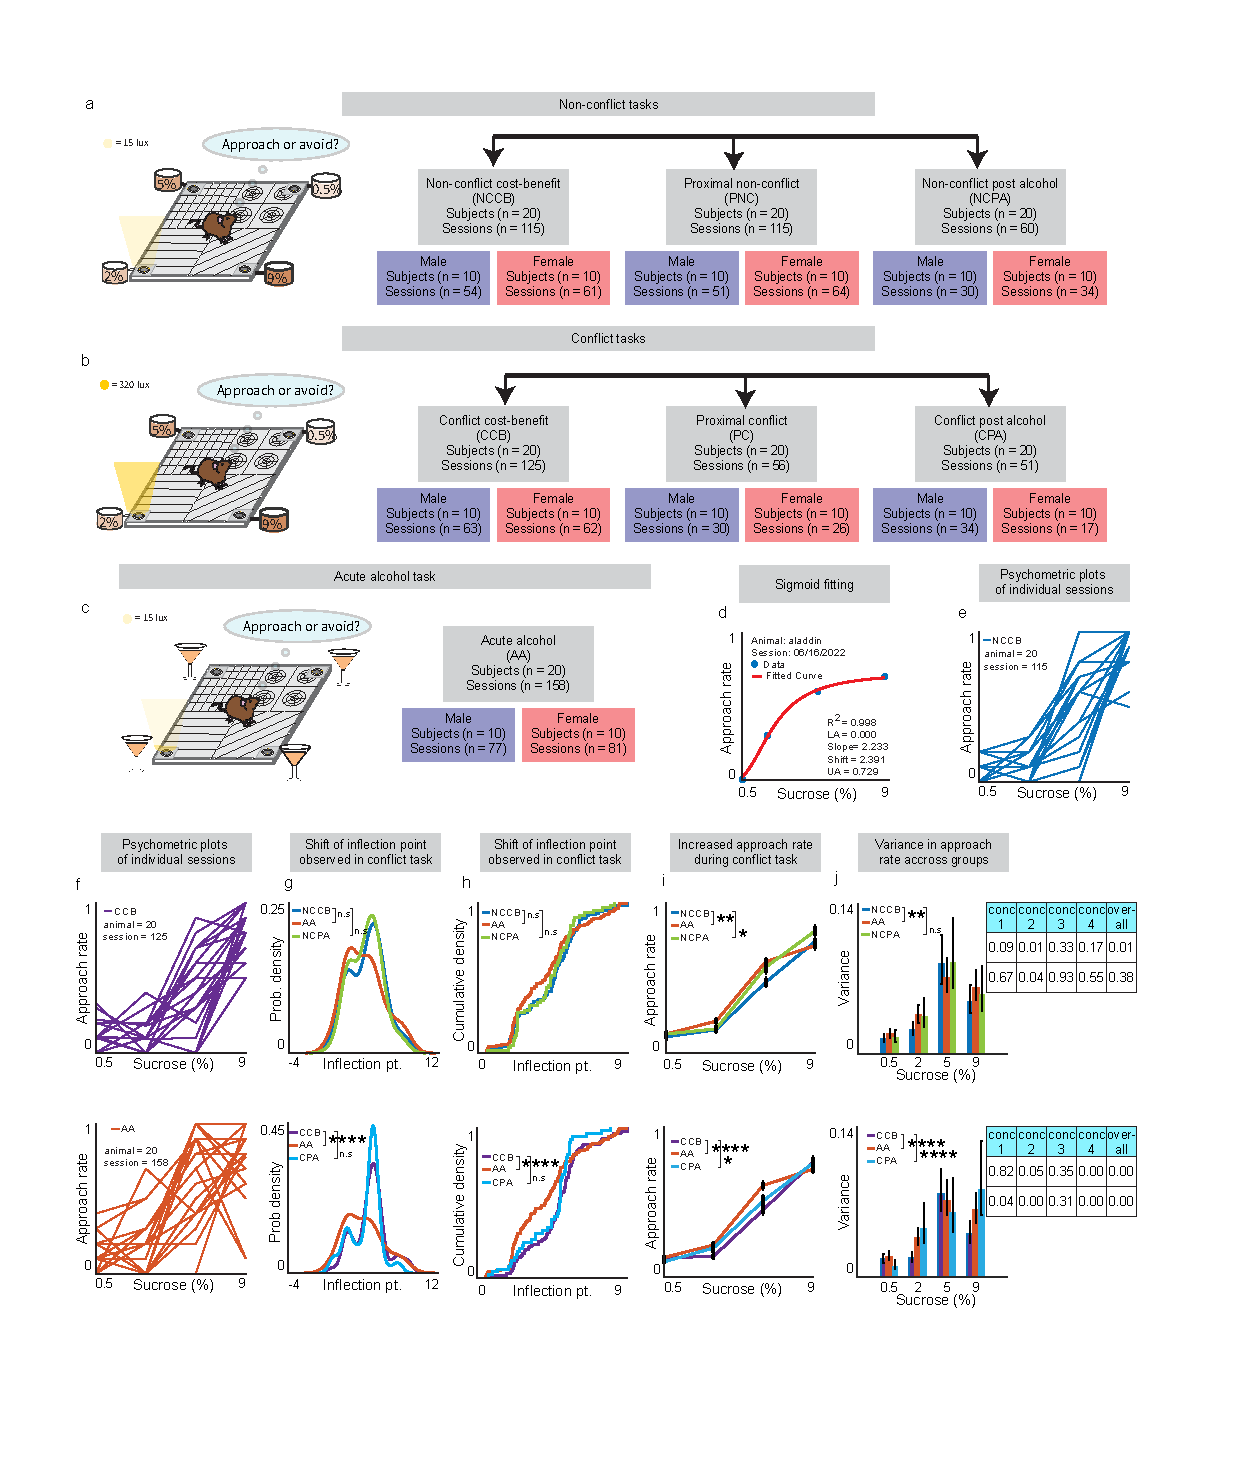
\includegraphics[width=\textwidth, trim=50 50 50 50]{Figs/Alcohol_main_1.pdf}
\end{figure}

\clearpage

\captionsetup{type=figure}  % Associate the following caption with the figure
\caption{\textbf{Overview and general analysis of behavioral tasks}. (a) Non-conflict, (b) conflict, and (c) acute alcohol cost-benefit tasks utilizing the RECORD setup where one of four sucrose concentrations are dispensed into a bowl surrounded by LED lights. (d) Example of psychometric function from a singular non-conflict cost benefit (NCCB) session, fitted with a 4-parameter logistic model $(f(x) = d + (a-d)/ (1 + (x/c)^b))$. Individual (n=20) psychometric functions demonstrating approach rate in non-conflict (e), conflict (f, top), and acute alcohol cost benefit tasks (f, bottom). (g, top) No significant difference in probability density of inflection points between acute alcohol (AA) compared to NCCB (p = 0.08) or NCPA (p = 0.75). (g, bottom) There are significant differences between AA, cost benefit conflict (CCB) tasks (KS test, p $<$ 0.0001), and no significant differences between AA and CPA (p = 0.17). (h) Inflection point distribution represented as a cumulative density function. (i, top) When comparing NCCB to AA (p = 0.001) and NCPA to NCCB (p = 0.05) approach rates are significantly different. (i, bottom) Similarly, comparing CCB to AA (p $<$ 0.0001) and CCB to CPA (p = 0.04) approach rates are also significantly different. (j) Variance in approach rate, with error bars depicting upper and lower confidence intervals with 95\% significance, show significance between NCCB and AA tasks (F-test, p = 0.0096), and CCB and AA tasks (F-test, p $<$ 0.0001).}
\label{fig:alcohol_main_1}

\vspace{1em}

\noindent\textbf{Sex differences to alcohol}\\
Looking at individual functions formed during NCCB then AA split by sex it seems that males generate more abnormal psychometric functions during AA task performance than females (\hyperref[fig:alcohol_main_2]{Fig. 2a, b, top} male, bottom female for all figures). Examining the distribution of inflection points across males and females we see a significant left shift in the male distribution compared to NCCB (\hyperref[fig:alcohol_main_2]{Fig. 2c, top}, p = 0.004) while females had no significant changes in the inflection point distribution (\hyperref[fig:alcohol_main_2]{Fig. 2c, bottom}). This was corroborated by analyzing the cumulative density functions (\hyperref[fig:alcohol_main_2]{Fig. 2d}). Approach rates for males during AA task performance were significantly increased when compared to NCCB (\hyperref[fig:alcohol_main_2]{Fig. 2e, top}, \hyperref[fig:Alcohol_SI_2]{Supplemental Fig. 2c left}, p $<$ 0.0001), while females had no significant differences across NCCB, NCPA, and AA (\hyperref[fig:alcohol_main_2]{Fig. 2e, bottom,} \hyperref[fig:Alcohol_SI_2]{Supplemental Fig. 2c, right}). Individual psychometric functions are similarly impacted across sex during AA task performance compared to CCB task performance (\hyperref[fig:alcohol_main_2]{Fig. 2f}). Similarly to NCCB and NCPA, the AA distribution was only significantly shifted in males across both density distributions and cumulative density functions (\hyperref[fig:alcohol_main_2]{Fig. 2g, h}, males AA compared to CCB, p $<$ 0.0001). There was also significant variation in males between CCB and AA task performance, but no such significant variation was observed in females (\hyperref[fig:Alcohol_SI_2]{Supplemental Fig. 2f}, CCB vs AA: p $<$ 0.0001 males, CCB vs. CPA: p $<$ 0.0001 males).

\begin{figure}
  \centering
  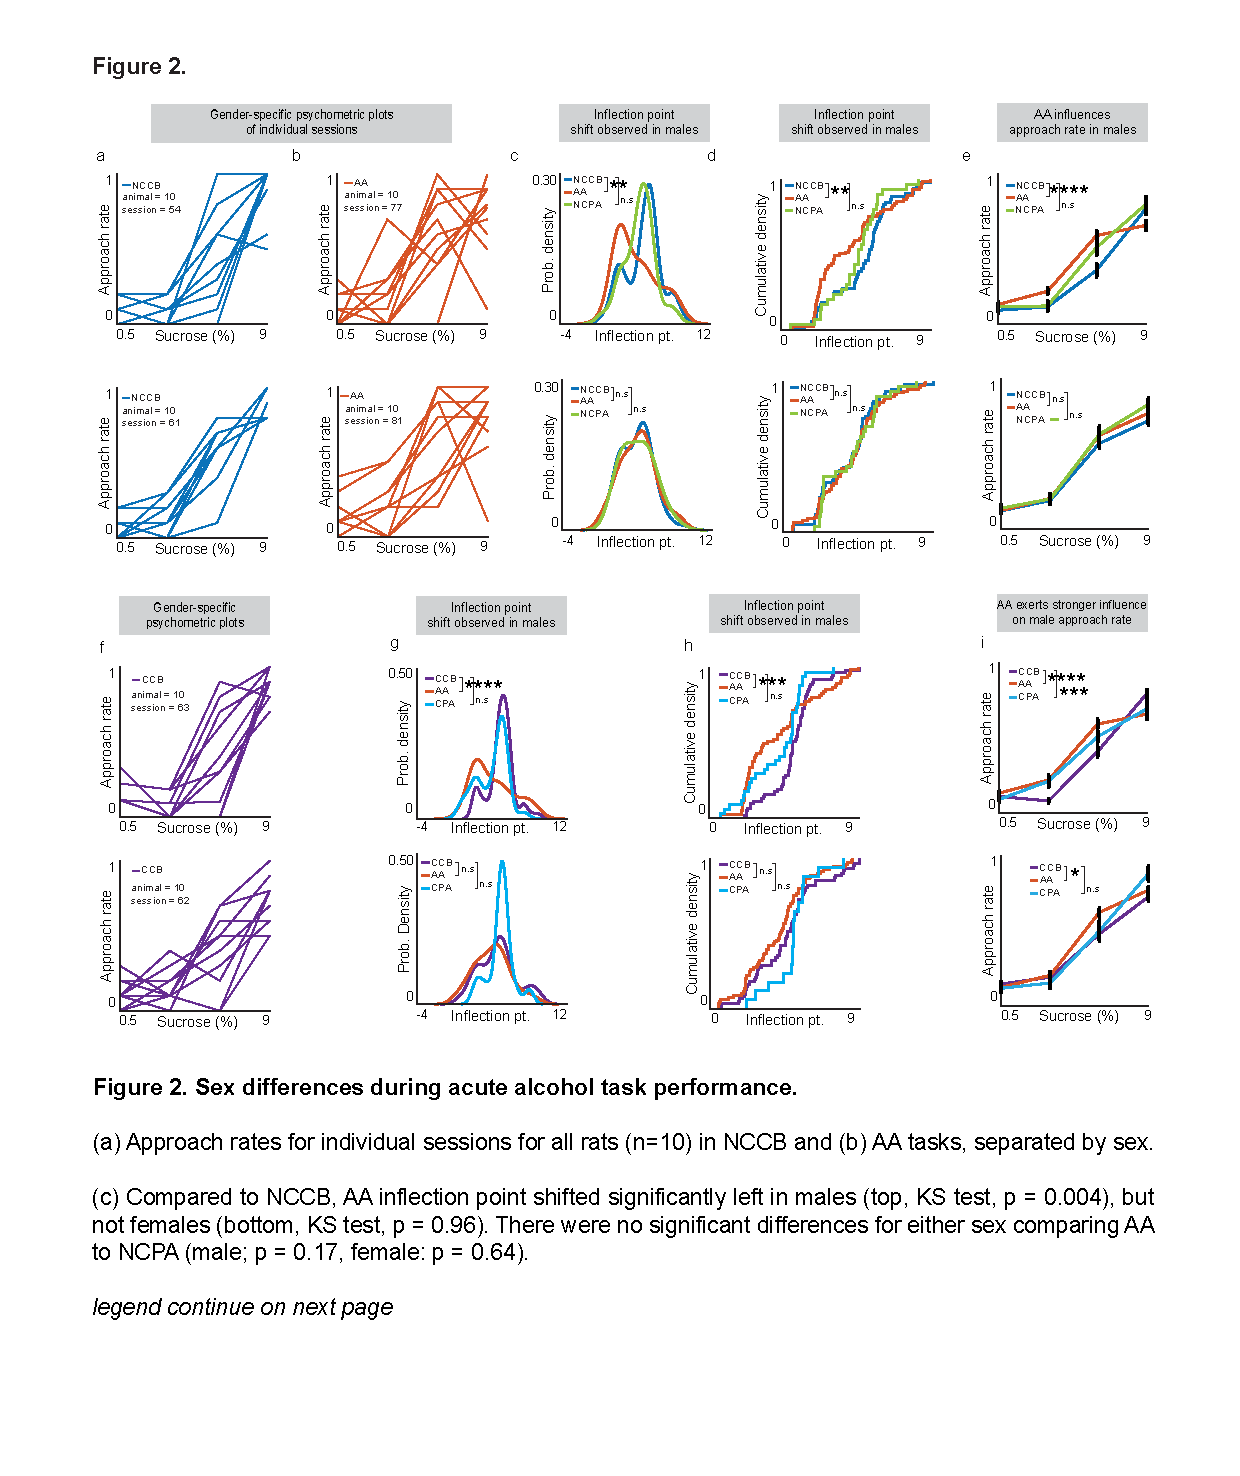
\includegraphics[width=\textwidth, trim=50 100 50 100]{Figs/Alcohol_main_2.pdf}
\end{figure}

\clearpage

\captionsetup{type=figure}  % Associate the following caption with the figure
\caption{\textbf{Sex differences during acute alcohol task performance.} (a) Approach rates for individual sessions for all rats (n=10) in NCCB and (b) AA tasks, separated by sex. (c) Compared to NCCB, AA inflection point shifted significantly left in males (top, KS test, p = 0.004), but not females (bottom, KS test, p = 0.96). (d) There were no significant differences for either sex comparing AA to NCPA (male; p = 0.17, female: p = 0.64). Cumulative density function plots of the distributions in (c). (e) Approach rate is significantly different between NCCB and AA for males (MANOVA, p $<$ 0.0001, top) but not females (MANOVA, p = 0.47, bottom). (f) Approach rates of individual sessions for rats split by sex (n = 10 males, n = 10 females) in CCB. (g) Compared to CCB, AA inflection point is significantly shifted left in males (KS test, p $<$ 0.0001) but not in females (KS test, p = 0.211) and again there was so significant difference when comparing CCB to CPA in either sex. (h) Inflection point distribution represented as a cumulative density function. (i) In CCB vs AA tasks, approach rate is significantly different in males (MANOVA, p $<$ 0.0001) and females (p = 0.0134) in CCB vs AA tasks with males also having significantly approach rates between CCB and CPA (p = 0.0007) unlike females (p = 0.1).}
\label{fig:alcohol_main_2}

\vspace{1em}

\noindent\textbf{Alcohol alters time spent in reward zones}\\
Evaluating alternative behaviors during task performance, we measured the time each rat spent in individual reward zones (\hyperref[fig:Alcohol_SI_2]{Supplemental Fig, 2a}). On average, rats performing AA spent more time in rewards zones containing 0.5\%, 2\% and 5\% sucrose, but not 9\%, compared to NCCB (\hyperref[fig:Alcohol_SI_2]{Supplemental Fig 2b top}, MANOVA, p = 0.0002) and CCB with a significant difference between CCB and CPA (\hyperref[fig:Alcohol_SI_2]{Supplemental Fig 2b bottom}, MANOVA, CCB compared to AA p $<$ 0.0001, CCB compared to CPA p $<$ 0.0001). Additionally, probability density plots of time spent in reward zones revealed that alcohol induced shifts significantly different from NCCB (\hyperref[fig:Alcohol_SI_2]{Supplemental Fig 2c top}, KS test, p = 0.003) and CCB (\hyperref[fig:Alcohol_SI_2]{Supplemental Fig 2c bottom}, KS test, p = 0.004). When split across genders, males spend significantly more time in reward zones (\hyperref[fig:Alcohol_SI_2]{Supplemental Fig 2e top}, MANOVA, p $<$ 0.0001) and significantly altered probability density shifts (\hyperref[fig:Alcohol_SI_2]{Supplemental Fig 2f top}, KS test, p = 0.005) when completing an AA versus NCCB. Similar trends are observed when males, but not females, demonstrate increased time in reward zones during CCB task performance (\hyperref[fig:Alcohol_SI_2]{Supplemental Fig 2h top}, MANOVA, p $<$ 0.0001) when performing AA compared to CCB. Males also (\hyperref[fig:Alcohol_SI_2]{Supplemental Fig 2i top}, KS test, p = 0.009) while there were no significant differences between distributions in females (\hyperref[fig:Alcohol_SI_2]{Supplemental Fig. 2i, bottom}).

\vspace{1em}

\noindent\textbf{Identifying abnormal task performance in individuals using psychometric functions}\\
The psychometric functions formed during behavioral task performance across sessions may be a helpful marker for identifying individuals who are impacted by alcohol presentation and consumption (\hyperref[fig:Alcohol_SI_3]{Supplemental Fig. 3a}). Across all tasks, animals are considered “abnormal” when the proportion of sigmoidal functions formed is less than 70\% (which is the same standard we used for our initial publication where we develop and validate the RECORD system\cite{ibanez2024record} of non-alcohol conditions, determined using the chi-square (\hyperref[fig:alcohol_main_3]{Fig. 3a}). Non-abnormal animals, in contrast, seem to maintain more consistent sigmoid-shaped functions across task types (\hyperref[fig:alcohol_main_3]{Fig. 3b}). We identified 7 abnormal males (\hyperref[fig:alcohol_main_3]{Fig. 3c left}) and 2 abnormal females (\hyperref[fig:alcohol_main_3]{Fig. 3c right}). This difference between the sexes was determined to be significant using a chi-square test (\hyperref[fig:alcohol_main_3]{Fig. 3d}, p=0.025). Further, only one male and 3 females had less than 70\% of sigmoidal sessions during both NCCB (\hyperref[fig:Alcohol_SI_3]{supplemental Fig. 3b-c}) and CCB tasks (\hyperref[fig:Alcohol_SI_3]{supplemental Fig. 3d-e}).

\begin{figure}[H] % [htbp]
  \centering
  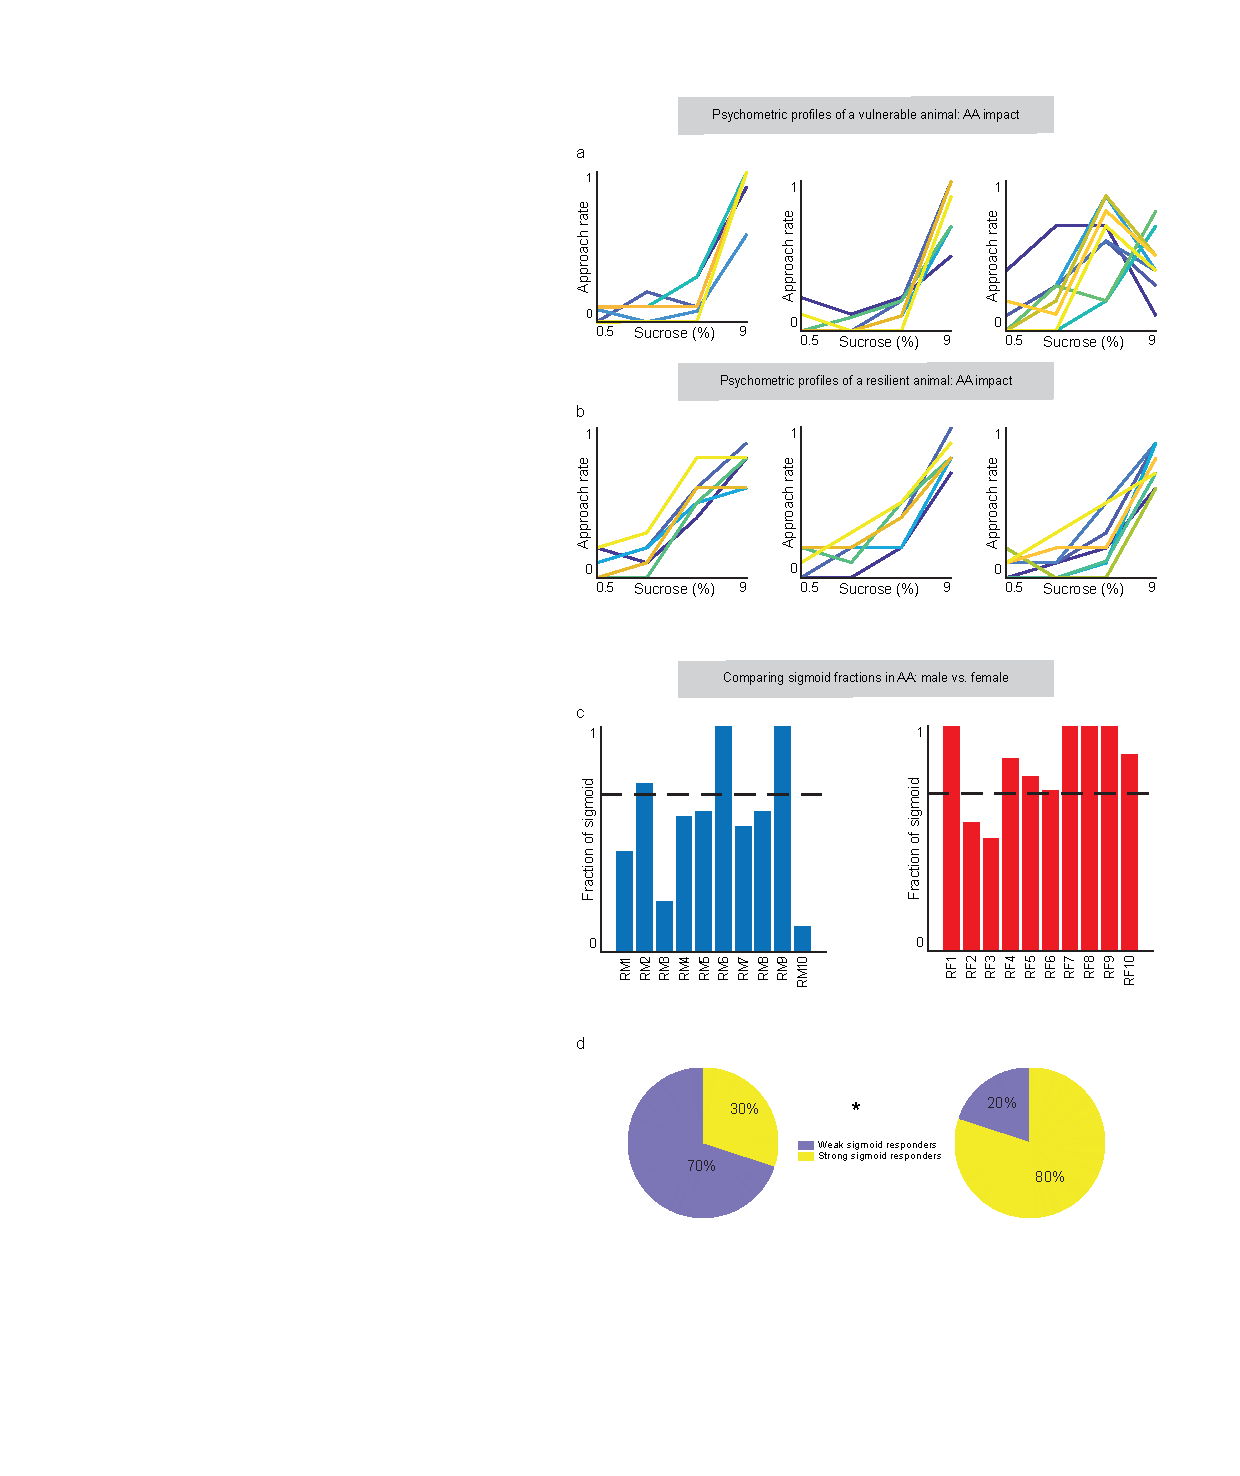
\includegraphics[width=\textwidth, trim=50 50 50 50]{Figs/Alcohol_main_3.pdf}
\end{figure}

\captionsetup{type=figure}
\caption{\textbf{Identifying abnormally performing subjects using their psychometric functions.} (a) Psychometric profiles depict abnormal task performance of a singular animal during NCCB, CCB, and AA tasks. (b) Non-abnormal singular animal psychometric profiles in NCCB, CCB, and AA tasks. (c) Two plots showing the fraction of sigmoid across all sessions of AA for individual males (n=10) and females (n=10), where the dashed line at y=0.7 indicates the threshold for fitting a sigmoid psychometric curve. (d) Pie charts depicting males (left) and females (right) with sigmoidal (blue) and non-sigmoidal (yellow) psychometric profiles. Males have significantly more non-sigmoidal sessions than females (chi-square test, p = 0.025).}
\label{fig:alcohol_main_3}

\vspace{1em}

\noindent\textbf{Alcohol effects the proximal cost benefit tasks}\\
Comparing psychometric functions of proximity tasks (\hyperref[fig:alcohol_main_4]{Fig. 4a}) to tasks completed soon after alcohol task performance (\hyperref[fig:alcohol_main_4]{Fig. 4b}), stark individual differences can be observed. Evaluating probability density plots across each stage of non-conflict cost benefit task, no significant difference is observed. When comparing probability density plots between each stage of conflict cost benefit task, a significant difference in peaks between CCB and PC (\hyperref[fig:alcohol_main_4]{Fig. 4c bottom}, KS test, p $<$ 0.0001) is observed. When comparing NCCB to PNC (MANOVA, p= 0.0023) and NCPA (MANOVA, p=0.046), significantly different approach rates (\hyperref[fig:alcohol_main_4]{Fig. 4e top}) were observed. While approach rates for each stage of this task follow an overall trend of increased acceptance as reward increases, only NCCB compared to PNC retain significant variability (\hyperref[fig:alcohol_main_4]{Fig. 4f top}, F-test, p=0.0015). Evaluating approach rate across each stage of the conflict cost benefit task, both PC (\hyperref[fig:alcohol_main_4]{Fig. 4d bottom}, MANOVA, p $<$ 0.0001) and CPA (\hyperref[fig:alcohol_main_4]{Fig. 4d bottom}, MANOVA, p=0.0413) were significantly different from CCB. Variance was also significantly different when comparing PC (\hyperref[fig:alcohol_main_4]{Fig. 4e bottom}, F-test, p $<$ 0.0001) and CPA (\hyperref[fig:alcohol_main_4]{Fig. 4e bottom}, F-test, p $<$ 0.0001) to CCB.

\begin{figure}[H] % [htbp]
  \centering
  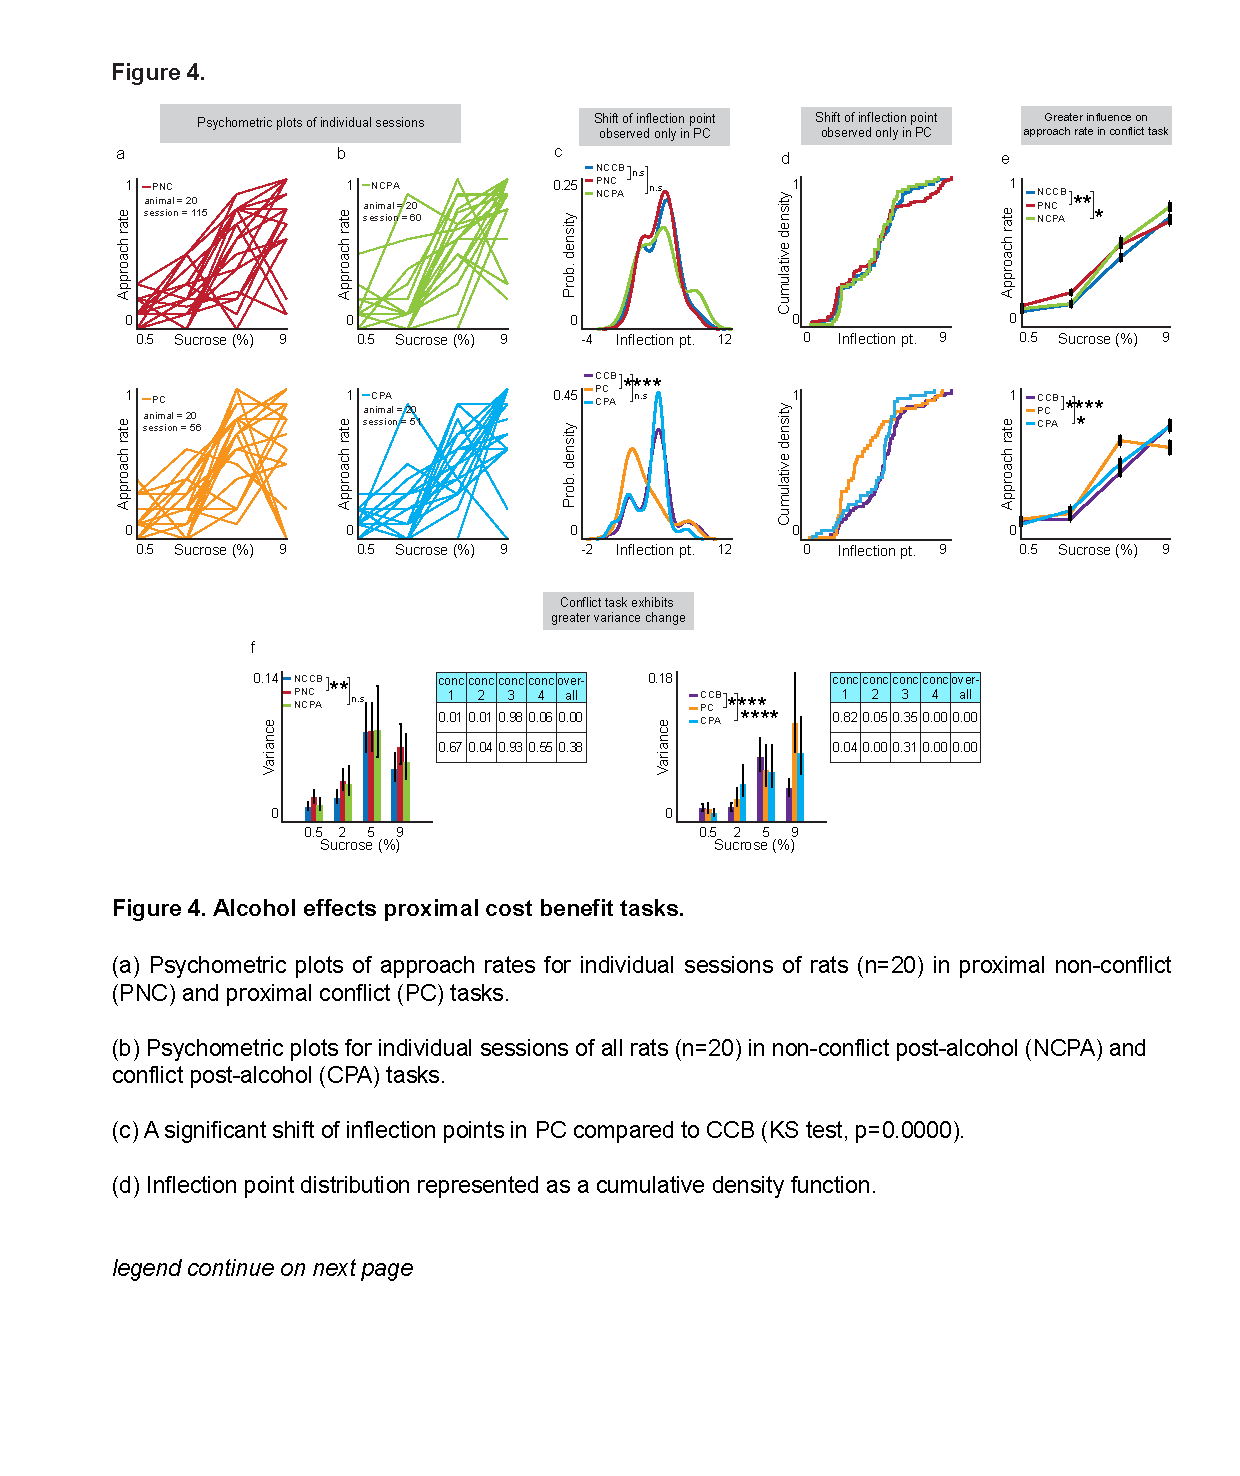
\includegraphics[width=\textwidth, trim=50 50 50 50]{Figs/Alcohol_main_4.pdf}
\end{figure}

\captionsetup{type=figure}
\caption{\textbf{Alcohol effects proximal cost benefit tasks.} (a) Psychometric plots of approach rates for individual sessions of rats (n=20) in proximal non-conflict (PNC) and proximal conflict (PC) tasks. (b) Psychometric plots for individual sessions of all rats (n=20) in non-conflict post-alcohol (NCPA) and conflict post-alcohol (CPA) tasks. (c) A significant shift of inflection points in PC compared to CCB (KS test, p=0.0000). (d) Inflection point distribution represented as a cumulative density function. (e) Approach rates were significantly different across all task types (NCCB vs. PNC: p = 0.002, NCCB vs NCPA; p = 0.05, CCB vs PC; p $<$ 0.0001, CCB vs CPA: 0.04). (f) Significant difference in variance between NCCB and PNC in both males (F-test, p = 0.015) and females (F-test, p = 0.0153, f, left). Significant variance in CCB vs PC (F-test, p $<$ 0.0001) and CPA (F-test, p $<$ 0.0001) task performance (f, right).}
\label{fig:alcohol_main_4}

\vspace{1em}

\noindent\textbf{Sex differences are observed during the proximal tasks}\\
Comparison of individual psychometric functions, separated by sex, across PNC (\hyperref[fig:alcohol_main_5]{Fig. 5a}) and NCPA (\hyperref[fig:alcohol_main_5]{Fig. 5b}). There were no significant differences in inflection point distributions for PNC task performance compared to NCCB and NCPA (\hyperref[fig:alcohol_main_5]{Fig. 5c}). Males also demonstrate shifted approach rates in PNC (\hyperref[fig:alcohol_main_5]{Fig. 5d top}, MANOVA, p $<$ 0.0001), while females do not. Comparisons between NCCB and PNC display significantly different variance in both male (\hyperref[fig:alcohol_main_5]{Fig. 5e top}, F-test, p=0.015) and females (\hyperref[fig:alcohol_main_5]{Fig. 5e bottom}, F-test, p=0.0153). Individual psychometric functions from PC (\hyperref[fig:alcohol_main_5]{Fig. 5f left}) and CPA (\hyperref[fig:alcohol_main_5]{Fig. 5g right}) can be evaluated based on sex. Strikingly, both males (\hyperref[fig:alcohol_main_5]{Fig. 5h top}, KS test, p=0.002) and females (\hyperref[fig:alcohol_main_5]{Fig. 5h bottom}, KS test, p=0.02) demonstrate significant alterations in density when comparing CCB and PC tasks. Notably, males (\hyperref[fig:alcohol_main_5]{Fig. 5j top}, MANOVA, p $<$ 0.0001) and females (\hyperref[fig:alcohol_main_5]{Fig. 5j bottom}, MANOVA, p=0.005) exhibit alterations in approach rate during proximal cost benefit conflict task.

\begin{figure}[H] % [htbp]
  \centering
  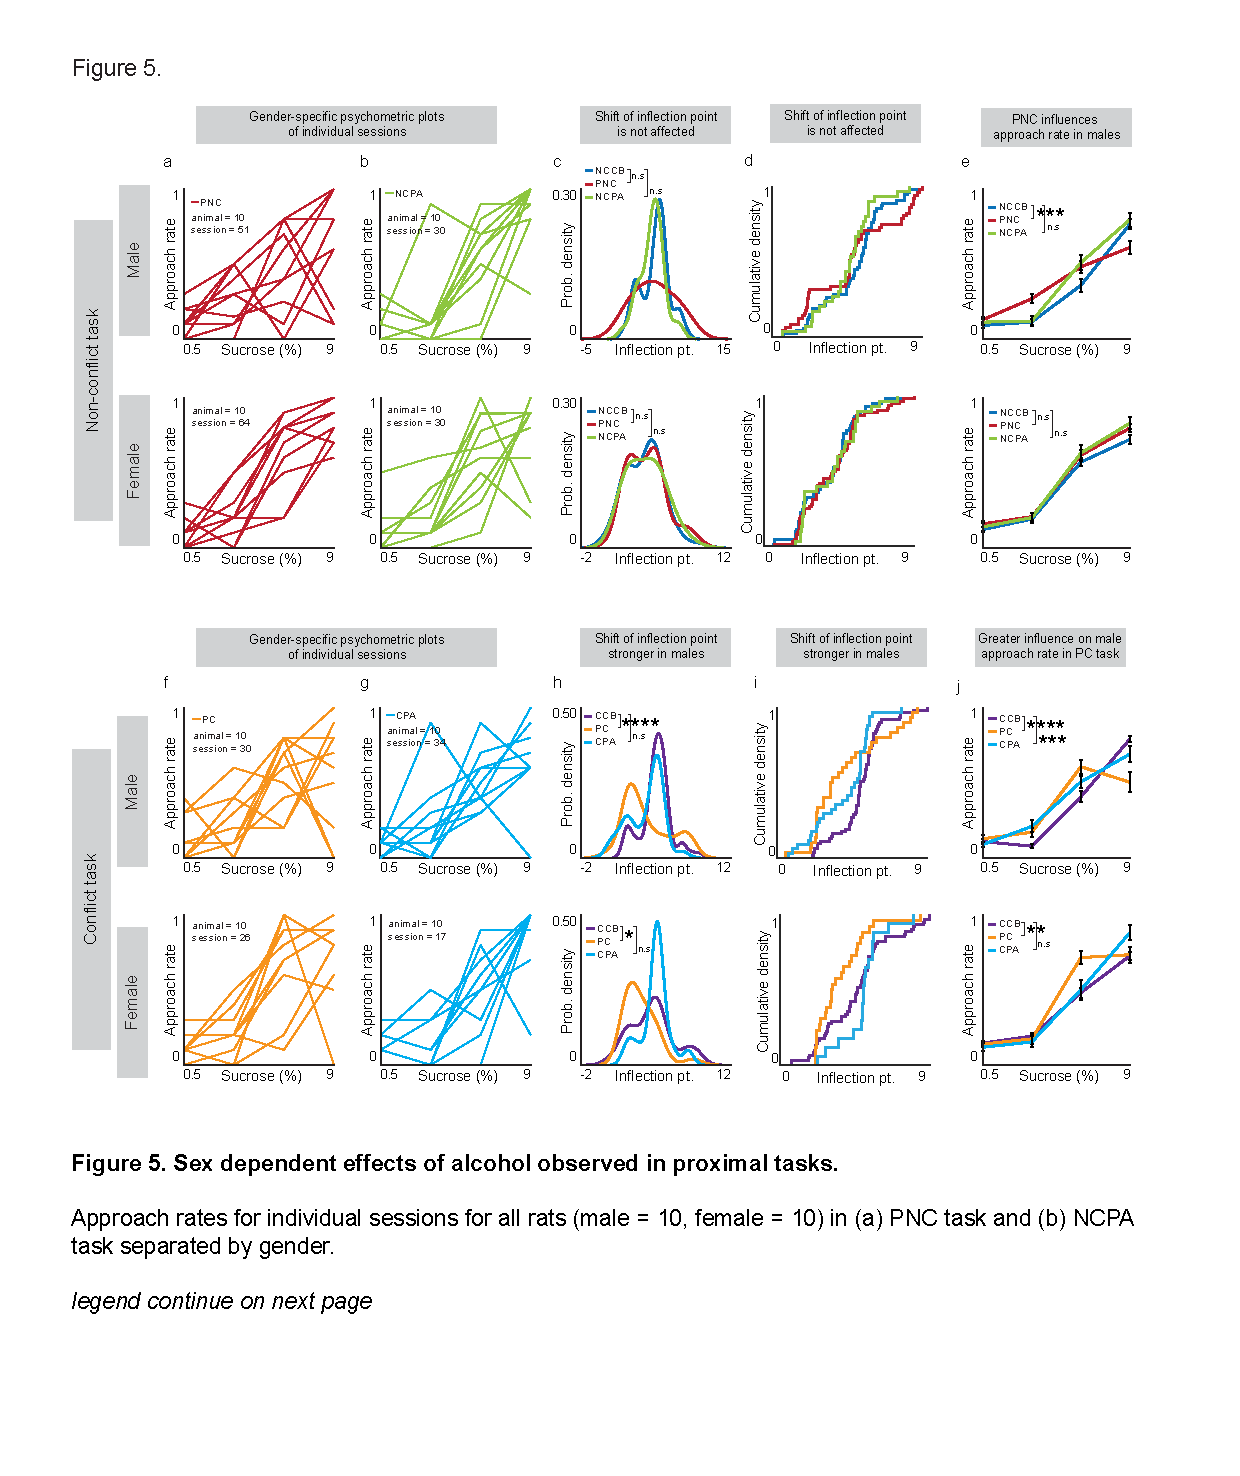
\includegraphics[width=\textwidth, trim=50 100 50 100]{Figs/Alcohol_main_5.pdf}
\end{figure}

\captionsetup{type=figure}
\caption{\textbf{Sex dependent effects of alcohol observed in proximal tasks.} Approach rates for individual sessions for all rats (male = 10, female = 10) in (a) PNC task and (b) NCPA task separated by gender. (c) No significant change in inflection point is observed across tasks or genders. (d) Inflection point distribution represented as a cumulative density function. (e) The difference in approach rates is statistically significant between NCCB and PNC in males (MANOVA, p $<$ 0.0001) but not females (NCCB vs PNC, MANOVA, p = 0.15). Approach rates for individual sessions for all rats (10 males, 10 females) in (f) PC and (g) CPA, separated by gender. (h) PC inflection point is significantly changed compared to CCB in both males (CCB vs. PC: KS test, p = 0.002) and females (CCB vs. PC: KS test, p = 0.02). (i) Inflection point distribution represented as a cumulative density function. (j) Differences in approach rate is statistically significant between CCB and PC across both males (MANOVA, p = 4.5992e-08) and females (MANOVA, p = 0.0046). Approach rates between CCB and CPA are significant in males (MANOVA, p = 6.5198e-04) but not in females (MANOVA, p = 0.1).}
\label{fig:alcohol_main_5}

\vspace{1em}

\noindent\textbf{Time spent in reward zone altered in the proximal tasks}\\
Proximal non-conflict task demonstrates significantly increased time spent in reward zones for 0.5, 2, and 5\% sucrose (\hyperref[fig:Alcohol_SI_4]{Supplemental Fig 4a top}, MANOVA, p=0.0209). However, both PNC (\hyperref[fig:Alcohol_SI_4]{Supplementary Fig 4b top}, KS test, p=0.0000) and NCPA (\hyperref[fig:Alcohol_SI_4]{Supplementary Fig 4b top}, KS test, p=0.0350) tasks display significant alterations in density when compared to NCCB. Proximal (\hyperref[fig:Alcohol_SI_4]{Supplementary Fig 4a bottom}, MANOVA, p=0.0001) and post alcohol (\hyperref[fig:Alcohol_SI_4]{Supplemental Fig 4a bottom}, MANOVA, p=0.0001) cost benefit conflict tasks demonstrate significantly increased time spent in reward zones containing 0.5\%, 2\%, and 5\% sucrose compared to CCB. When evaluating gendered effects of time spent in reward zones, males but not females demonstrated increased time spent in 0.5\%, 2\%, and 5\% sucrose during both PNC (\hyperref[fig:Alcohol_SI_4]{Supplementary Fig 4c top}, MANOVA, p=0.0021) and NCPA (\hyperref[fig:Alcohol_SI_4]{Supplementary Fig 4c top}, MANOVA, p=0.047). Males also exhibit increased density in PNC (\hyperref[fig:Alcohol_SI_4]{Supplemental Fig 4d top}, KS test, p=0.003) but not NPA tasks. This trend of increase time spent in 0.5\%, 2\%, and 5\% sucrose conserved, and male dominated in PC (\hyperref[fig:Alcohol_SI_4]{Supplemental Fig 4e top}, MANOVA, p $<$ 0.0001) and CPA (\hyperref[fig:Alcohol_SI_4]{Supplemental Fig 3e bottom}, MANOVA, p $<$ 0.0001) tasks. This is further supported by the significantly altered density peaks in males performing PC (\hyperref[fig:Alcohol_SI_4]{Supplemental Fig 4f top}, KS test, p $<$ 0.0001) and CPA (\hyperref[fig:Alcohol_SI_4]{Supplemental Fig 4f top}, KS test, p $<$ 0.0001).

\vspace{1em}

\noindent\textbf{Identification of continued non-sigmoidal function during the proximal tasks}\\
Interested in determining whether abnormal populations in proximal non-conflict and conflict tasks were gender exclusive, a chi squared test was used to quantify a 70\% difference in fraction of a sigmoid. Notably, half the males in PNC displayed behavioral abnormalities while all females displayed did not (\hyperref[fig:alcohol_main_6]{Fig. 6a-b}, chi-square test, p=0.0098). When comparing abnormal males and females in the context of NCPA, neither group was significant (\hyperref[fig:Alcohol_SI_4]{Supplementary Fig 4g-h}). During PC, males displayed greater instances of abnormalities (n=5) than females (n=2), but the two were not statistically different (\hyperref[fig:alcohol_main_6]{Fig. 6c-d}, chi-square test, p=0.16). Interestingly, in CPA both males and females exhibit equal numbers of abnormal individuals (\hyperref[fig:Alcohol_SI_4]{Supplemental Fig 4i-j}, chi-square test, p= 1.0).

\vspace{1em}

\begin{figure}[H]
  \centering
  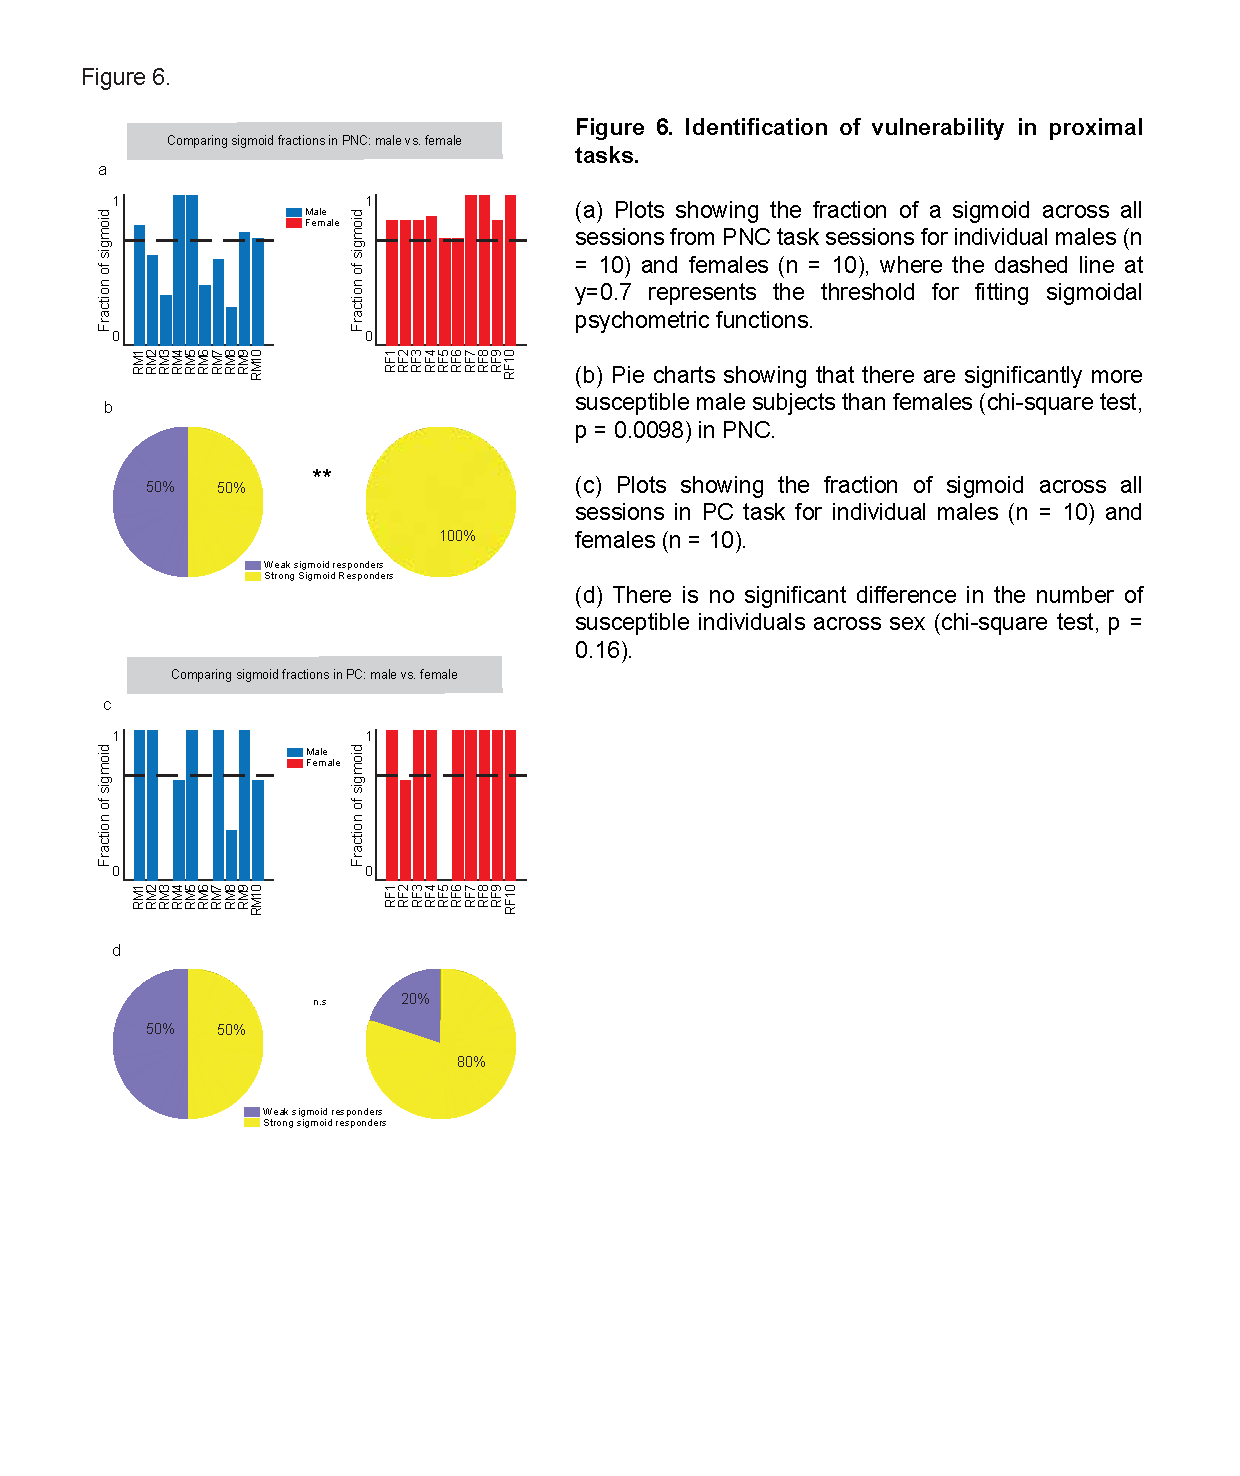
\includegraphics[width=\textwidth, trim=50 100 50 100]{Figs/Alcohol_main_6.pdf}
  \caption{\textbf{Identification of abnormal performance in proximal tasks.} (a) Plots showing the fraction of a sigmoid across all sessions from PNC task sessions for individual males (n = 10) and females (n = 10), where the dashed line at y=0.7 represents the threshold for fitting sigmoidal psychometric functions. (b) Pie charts showing that there are significantly more abnormal male subjects than females (chi-square test, p = 0.0098) in PNC. (c) Plots showing the fraction of sigmoid across all sessions in PC task for individual males (n = 10) and females (n = 10). (d) There is no significant difference in the number of abnormal individuals across sex (chi-square test, p = 0.16).}
  \label{fig:alcohol_main_6}
\end{figure}

\clearpage

\subsubsection{Discussion}

Overall, we introduced alcohol in inverse concentrations to an approach-avoid trade-off task. By presenting sucrose and alcohol in inverse concentrations (highest sucrose concentration with lowest alcohol concentration), rodents could minimize their exposure to alcohol while still attaining the attractive sucrose reward. However, we saw that rats had significantly different approach rates across various features once alcohol became integrated into the task environment (\hyperref[fig:alcohol_main_1]{Fig. 1}). When looking at approach rates for each level of reward the change in approach rate is driven by a higher approach rate for 2\% and 5\% sucrose, the moderate sucrose and alcohol combinations (\hyperref[fig:Alcohol_SI_1]{Supplemental Fig. 1}) as opposed to high alcohol (0.5\%) or high sucrose concentration (9\%). When we looked at sex differences after introducing alcohol into the task environment, we found that males were significantly affected by the presence of alcohol, shifting their approach rates towards 2\% and 5\% while females were minimally affected (\hyperref[fig:alcohol_main_2]{Fig. 2}). One potential reason males start approaching 2\% and 5\% more while decreasing their approach for 9\% could be that they view moderate sucrose with moderate alcohol more rewarding than either on their own, like how some people prefer mixed drinks or cocktails as opposed to strong spirits or soda.

\vspace{1em}

Alcohol also significantly increased the time spent in reward zones; this significance is also mostly driven by males (\hyperref[fig:alcohol_main_3]{Fig. 3}). We then used behavioral psychometric functions to try and delineate between rats that presented abnormal behaviors during the alcohol task and rats that did not. We looked at the proportion of sessions that were sigmoidal vs those that were not and identified seven males and three females that had less than 70\% of sessions that were sigmoidal (\hyperref[fig:alcohol_main_4]{Fig. 4}). Looking at task performance after alcohol consumption we saw that when compared to CCB and NCCB before acute alcohol, PC and PNC are significantly altered with the preference for 2\% and 5\% being retained while the preference for 9\% occasionally dips below pre-alcohol levels (\hyperref[fig:alcohol_main_5]{Fig. 5}, \hyperref[fig:alcohol_main_6]{6}). We also found that markers of acute alcohol abnormality persist for five male rats and two female rats after alcohol task performance (\hyperref[fig:alcohol_main_6]{Fig. 6}).

\vspace{1em}

In the United States, half of adults reported consuming alcohol in the thirty days prior to being surveyed, 17\% of adults reported binge drinking, and 6\% reported drinking heavily\cite{centers2008behavioral}. Alcohol abuse is characterized by persistent, habitual drinking despite social, medical, and economic decline. Interestingly, despite how prevalent drinking alcohol is, most individuals who drink do not develop an alcohol use disorder\cite{kranzler2023overview}. Researchers, however, often face the difficulty of developing an ethologically relevant rodent alcohol task since alcohol is aversive to rodents\cite{pautassi2011ethanol}.

\vspace{1em}

Many other rodent paradigms looking at alcohol use and decision-making examine binge drinking patterns or chronic alcohol consumption\cite{strong2010binge, jury2017sex}. Additionally, these conditions are typically done using a water and ethanol mixture without sucrose\cite{crabbe2009line, hwa2011persistent}. These studies generally find that female rodents are the ones that consume more sucrose\cite{strong2010binge, hwa2011persistent, jury2017sex}. In our task, we found that presenting a sucrose-alcohol mixture into the maze caused a significant change in how males perform the task, where they approached 2\% and 5\% sucrose more than in the non-alcohol task conditions. Females in our task did not demonstrate many significant differences whether alcohol was present or not. Overall, this research, potentially due to the approach-avoid style task, mixture of alcohol with sucrose, and acute nature of the alcohol exposure finds a greater shift in male decision-making and behavior with minimal shifts observed in female rodents.

\vspace{1em}

This aversion has required the use of various approaches like forcing alcohol consumption\cite{thiele2014drinking, mendoza2018forced} or breeding animals genetically predisposed to alcohol consumption\cite{timme2020alcohol, borruto2021genetically, sauton2021interstrain}. Traditional forced alcohol models are effective in representing alcohol use disorder but are less suited for mimicking acute/social drinking. We sought to mimic acute drinking by offering differing concentrations of alcohol and using a paradigm where the alcohol can be approached (accepted) or avoided (rejected). We utilized our RECORD task environment to design a battery of tasks that incorporate elements commonly used including sweetened alcohol, cost-benefit trade-offs, and run-away paradigms. A notable strength of the RECORD system is the ability to offer a “gradient” of trade-offs within a single session.

\vspace{1em}

Future work exploring acute alcohol consumption could use a similar task setup with in vivo recordings to uncover correlated neural activity as the task is performed. Exploring these neuronal recordings and other alcohol factors, like delivering chronic alcohol, could give further insight into the physiological activities underlying acute/social alcohol consumption and how it may differ in individuals with alcohol use disorder. Additionally, further exploration into identifying individuals who are more impaired by alcohol through the alterations in psychometric functions and associated neural correlates could help identify at risk groups which may eventually lead to earlier interventions for those predisposed to alcohol use disorder.

\clearpage

\subsubsection{Data Availability}

The data used within this manuscript is available at \url{https://dataverse.harvard.edu/dataset.xhtml?persistentId=doi:10.7910/DVN/YVPYUJ}.

\subsubsection{Code Availability}
All codes used for this manuscript can be accessed with the following link:\\
\url{https://github.com/atanugiri/Alcohol-Project/tree/main}

\clearpage

\subsubsection{Supplementary information}

\clearpage

\begin{suppfigure}
\centering
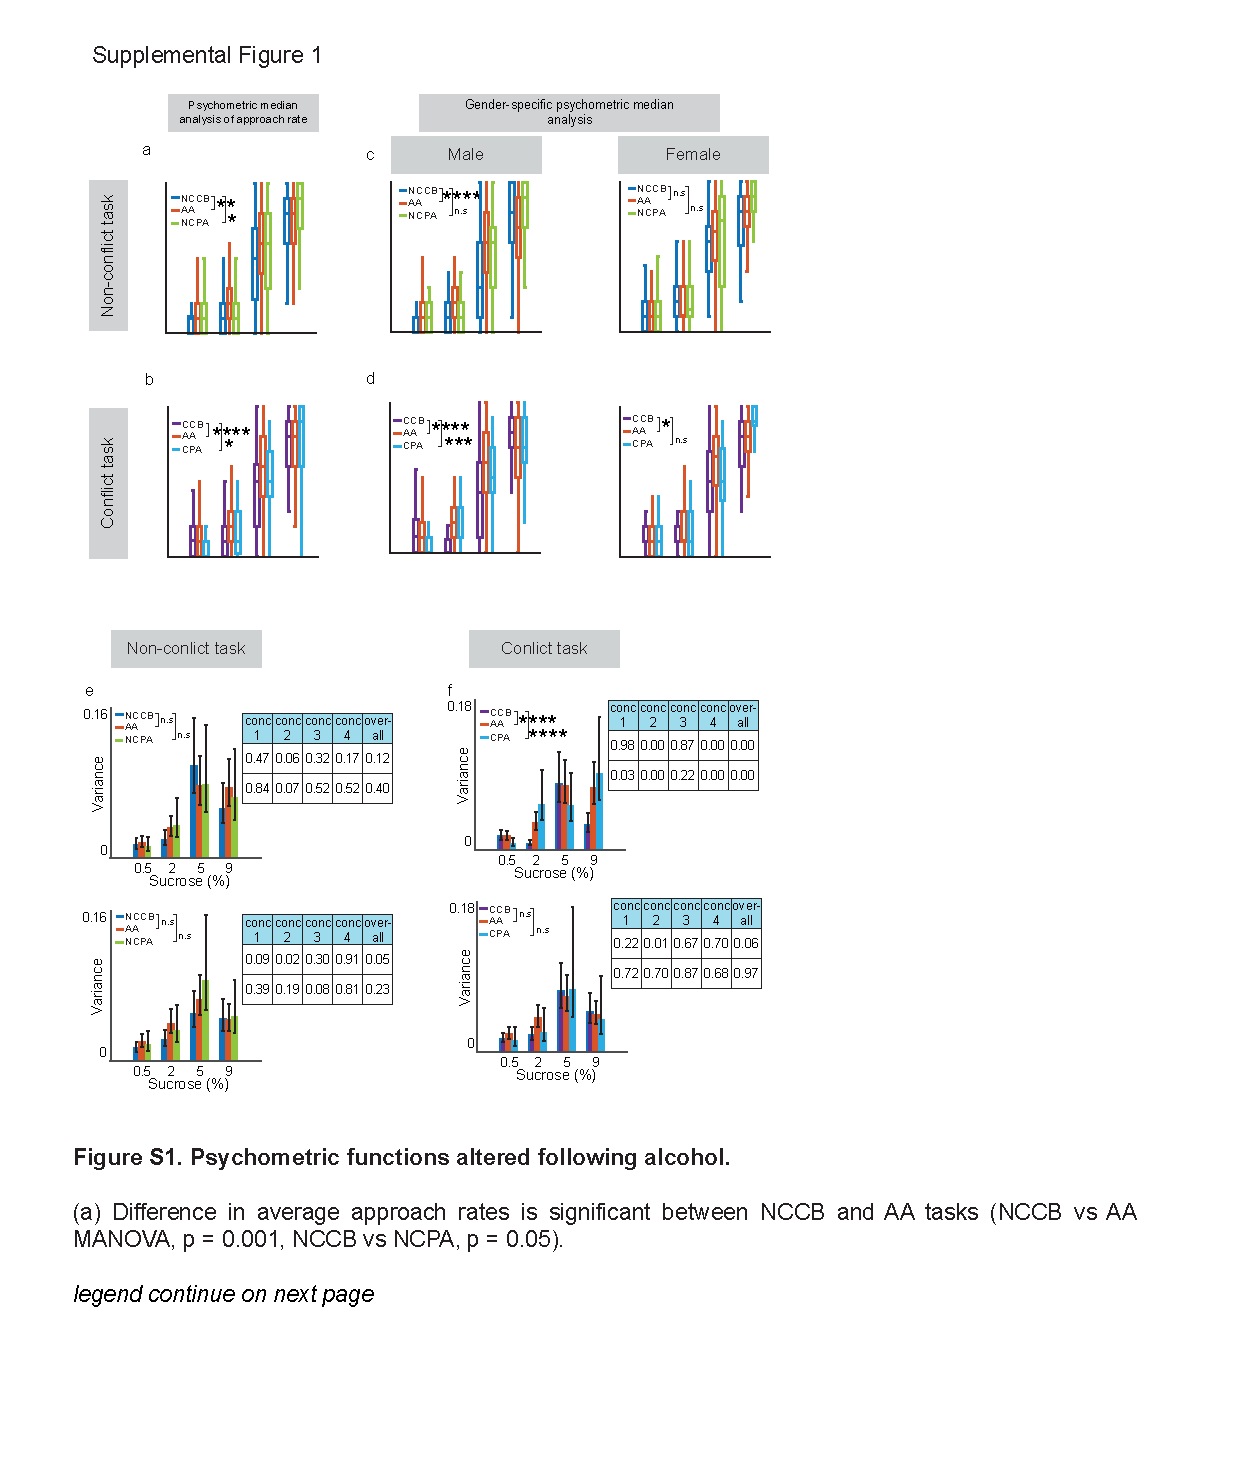
\includegraphics[width=\textwidth, trim=50 100 50 100]{Figs/Alcohol_SI_1.pdf}
\label{fig:Alcohol_SI_1}
\end{suppfigure}

\clearpage

\begin{singlespace}
\noindent Figure S1.\textbf{Psychometric functions altered following alcohol.} (a) Difference in average approach rates is significant between NCCB and AA tasks (NCCB vs AA MANOVA, p = 0.001, NCCB vs NCPA, p = 0.05). (b) Differences between CCB vs. CPA and AA are significant (CCB vs AA, MANOVA, p $<$ 0.0001, CCB vs CPA, p = 0.04). (c) sex differences in approach during non-conflict tasks were only present in males NCCB vs AA (MANOVA, p $<$ 0.0001). (d) During conflict tasks, male approach rate was significantly different between CCB vs AA (p $<$ 0.0001) and CPA (p = 0.0007) while females had significantly different approach rates between CCB and AA (p = 0.01). (e) Variance in approach rate during non-conflict task is insignificant across both sexes. (f) Variance is significant during conflict tasks in males (p $<$ 0.0001 for both CCB vs AA and CCB vs CPA) but not females.
\end{singlespace}

\clearpage

\begin{suppfigure}
  \centering
  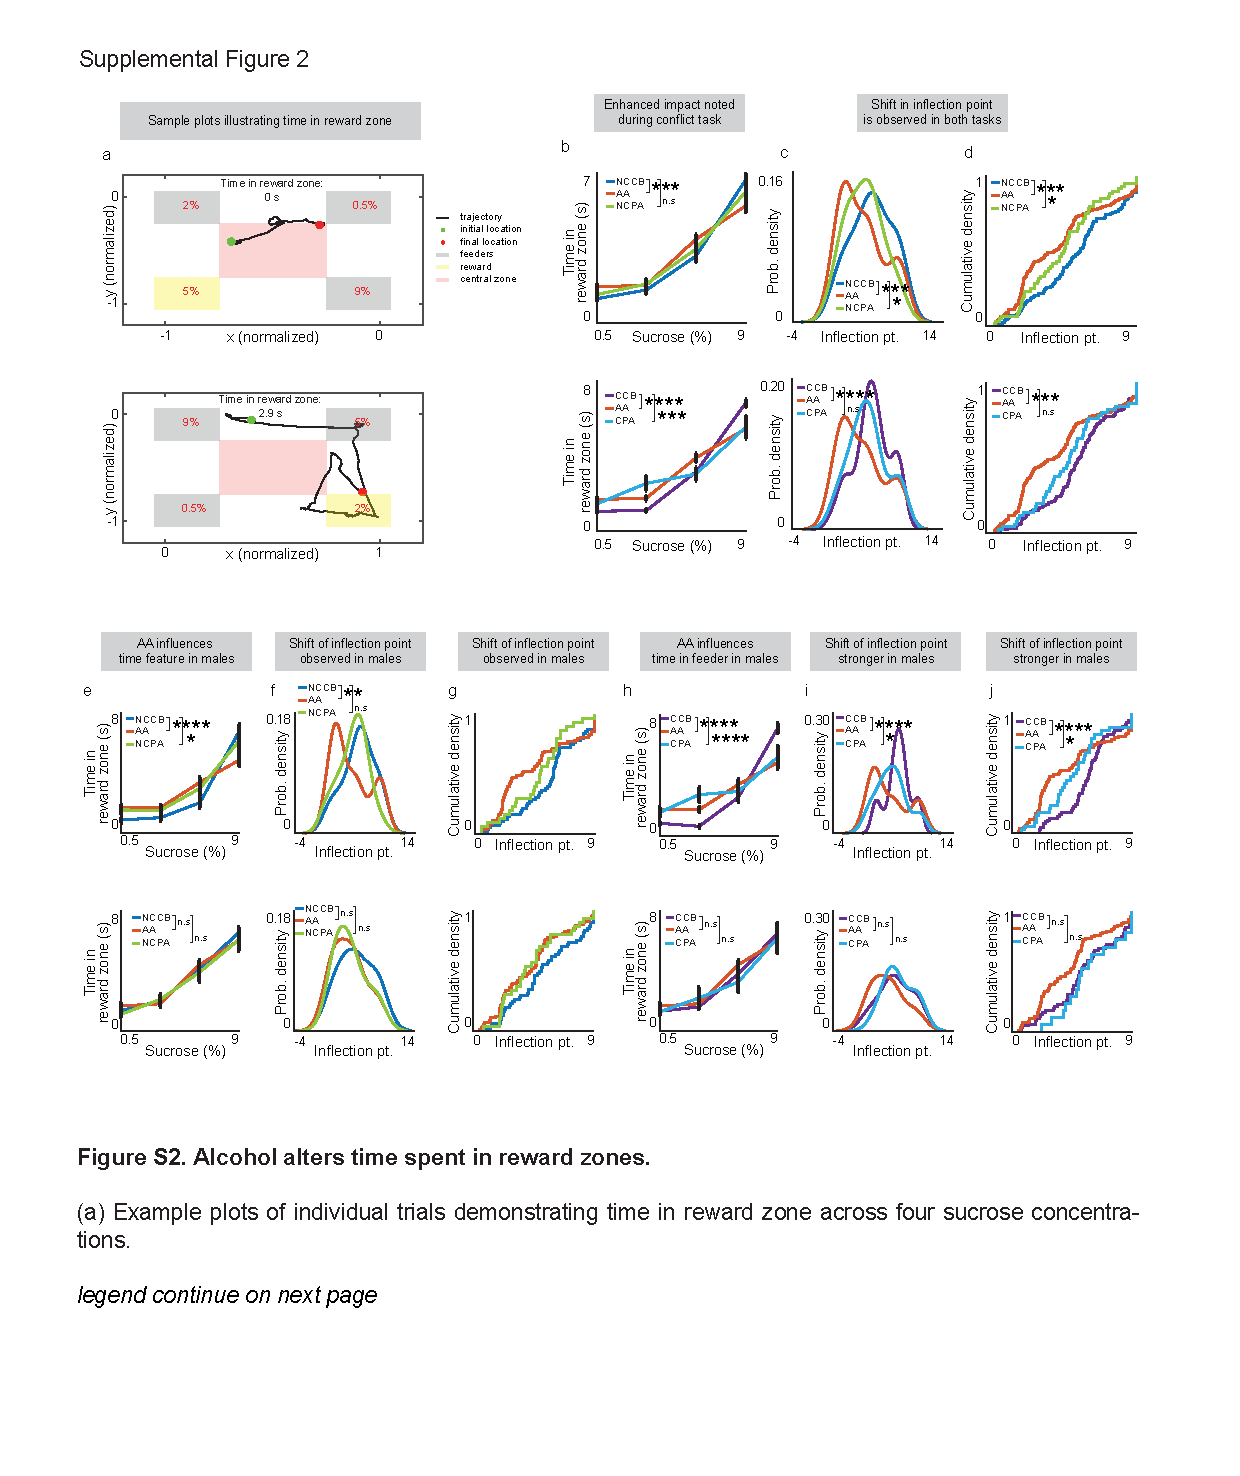
\includegraphics[width=\textwidth, trim=50 100 50 100]{Figs/Alcohol_SI_2.pdf}
  \label{fig:Alcohol_SI_2}
\end{suppfigure}

\clearpage

\begin{singlespace}
\noindent Figure S2.\textbf{Alcohol alters time spent in reward zones.} (a) Example plots of individual trials demonstrating time in reward zone across four sucrose concentrations. (b) Significantly different average time in reward zones between NCCB and AA tasks (MANOVA, p = 0.0002, NCCB vs NCPA, p = 0.05), and CCB and AA tasks (MANOVA, p $<$ 0.0001). (c) Inflection point is significantly different between NCCB and AA (KS test, p = 0.003) and CCB and AA tasks (KS test, p = 0.004). (d) Inflection point distribution represented as a cumulative density function. (e) Time in reward zone is significantly different between NCCB and AA tasks for males only (MANOVA, p $<$ 0.0001). (f) Inflection point is significantly different in male NCCB and AA tasks (KS test, p = 0.005). (g) Inflection point distribution represented as a cumulative density function. (h) Males display significantly different times spent in reward zones in CCB and AA (MANOVA, p $<$ 0.0001). (i) Males (KS test, p = 0.009) are also marked by significantly altered inflection points in CCB compared to AA. (j) Inflection point distribution represented as a cumulative density function.
\end{singlespace}

\clearpage

\begin{suppfigure}
  \centering
  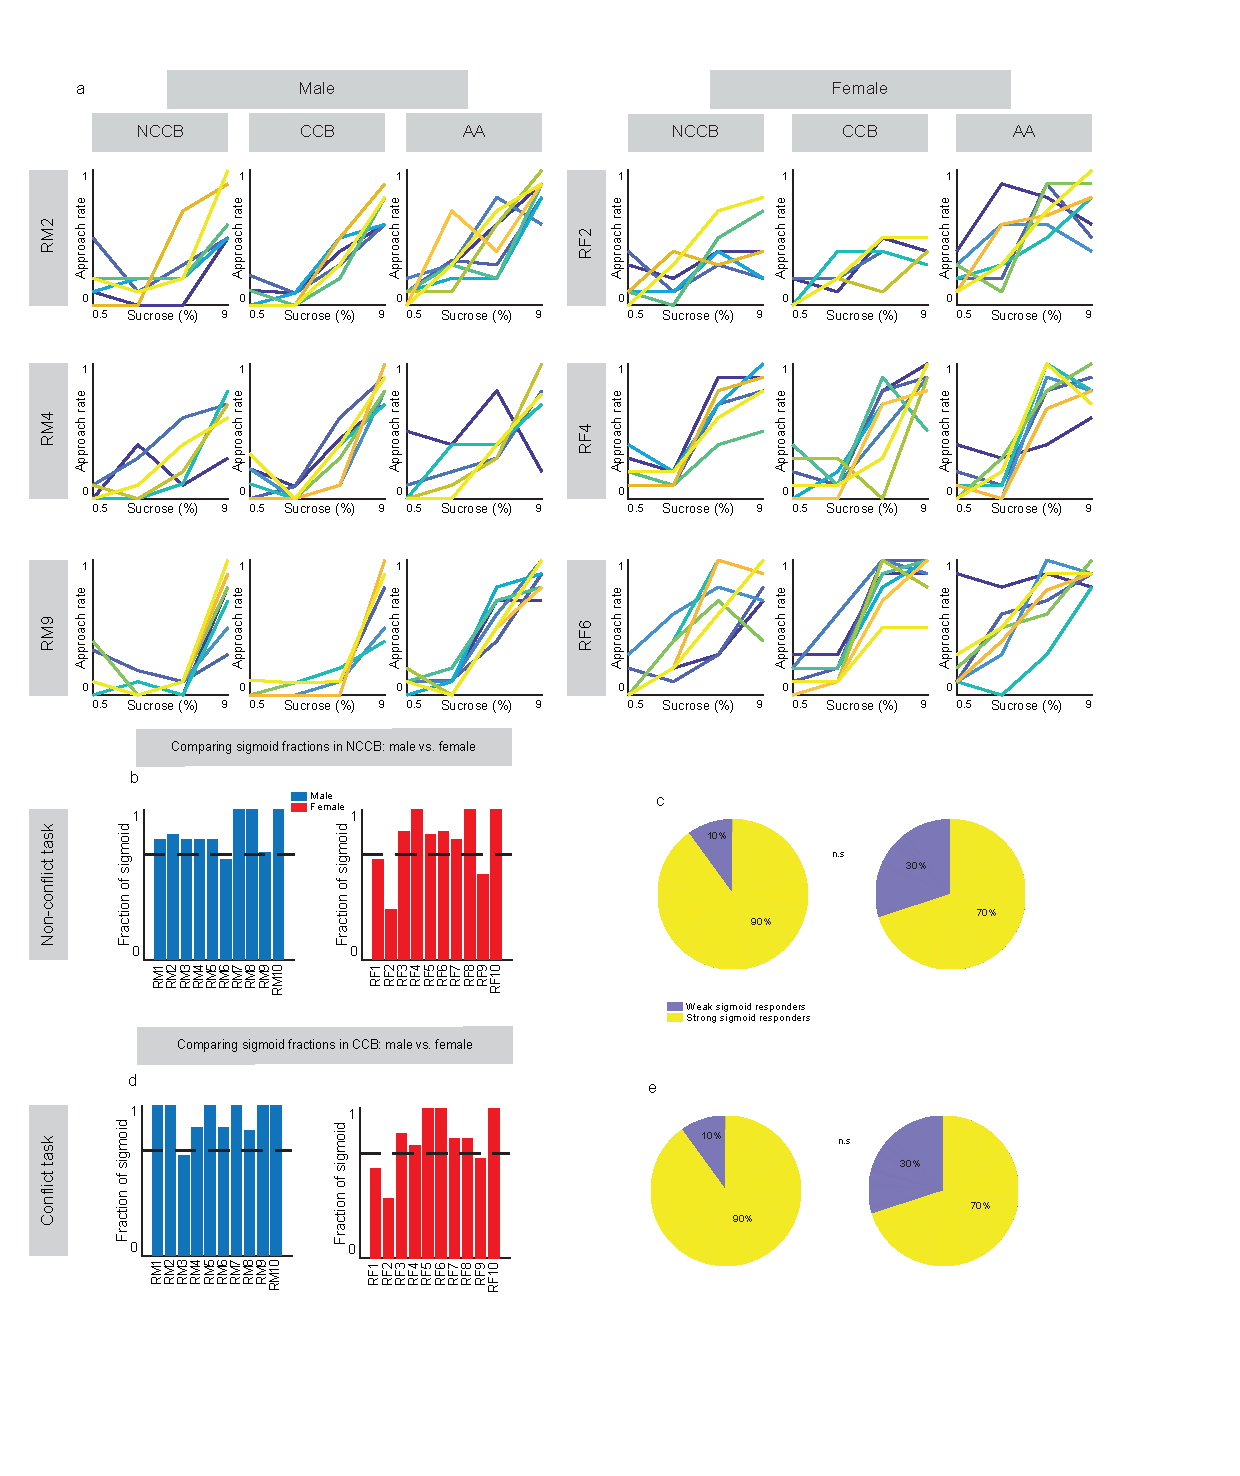
\includegraphics[width=\textwidth, trim=50 100 50 100]{Figs/Alcohol_SI_3.pdf}
  \label{fig:Alcohol_SI_3}
\end{suppfigure}

\clearpage

\begin{singlespace}
\noindent Figure S3. \textbf{Normal versus abnormal task performance in individuals following alcohol.} (a) Individual male and female psychometric profiles in NCCB, CCB, and AA tasks. (b) Two plots showing the fraction of sigmoid across all sessions in NCCB for individual males (n = 10) and females (n = 10), where there is no significant difference in (c) abnormality across genders (chi-square test, p = 0.2636). (d) Two plots showing the fraction of sigmoid across all sessions in CCB for individual males (n = 10) and females (n = 10), where there is no significant difference in (e) abnormality across genders (chi-square test, p = 0.26).
\end{singlespace}

\clearpage

\begin{suppfigure}
  \centering
  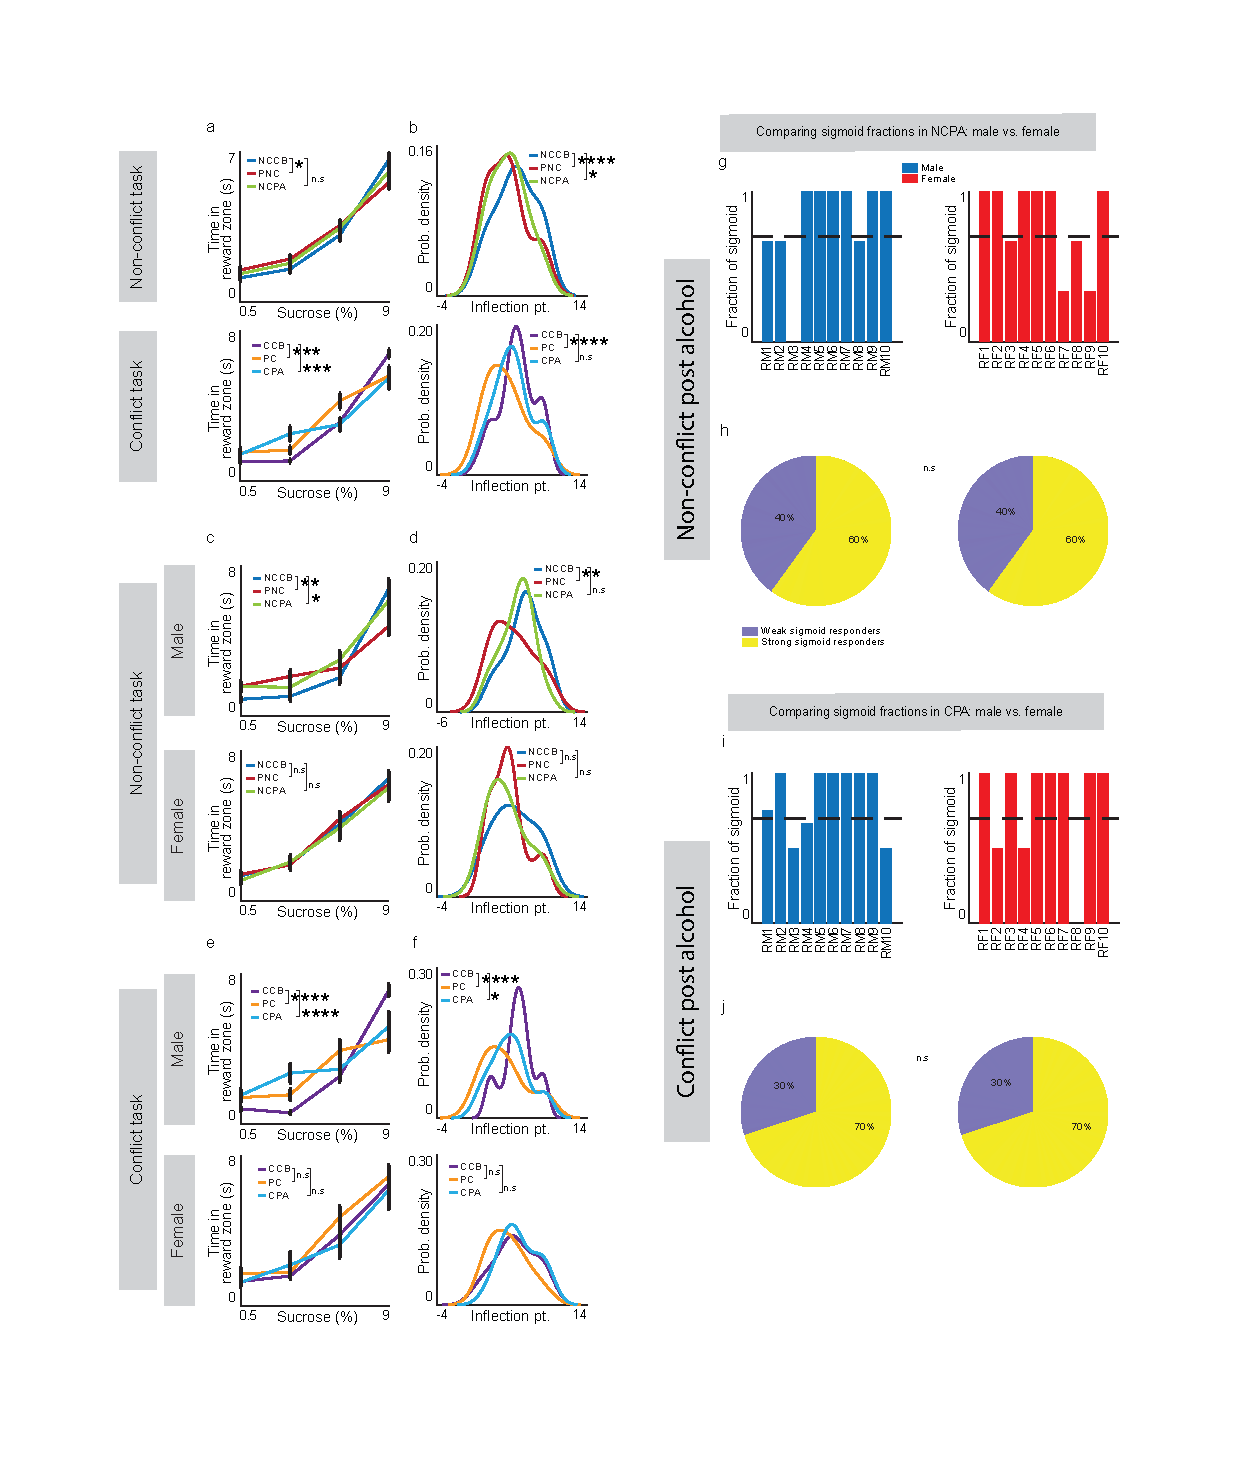
\includegraphics[width=\textwidth, trim=50 100 50 100]{Figs/Alcohol_SI_4.pdf}
  \label{fig:Alcohol_SI_4}
\end{suppfigure}

\clearpage

\begin{singlespace}
\noindent Figure S4. \textbf{Alcohol affects time and individual differences in non-alcohol related decision-making.} (a) Significantly different in time in reward zone in NCCB vs PNC (MANOVA, p = 0.0209), but not in NCCB vs NCPA (MANOVA, p = 0.6699). Both PC (MANOVA, p = 0.0001) and CPA (MANOVA, p = 0. 0001) tasks are significantly different from the CCB task. (b) Changes in inflection point are more prominent in NCCB vs PNC (KS test, p = 0.0000) than in NCCB vs NCPA (KS test, p = 0.0350). (c) Only CCB vs PC show a significant alteration in inflection point (KS test, p = 0.0000). PNC (MANOVA, p = 0.0021) and NCPA (MANOVA, p = 0.0474) compared to NCCB show a significant difference in time spent in reward zone across males only. (d) Only male PNC vs NCCB show a statistical difference in inflection point of kernel probability densities (KS test, p = 0.0030). (e) Males show significant difference in time spent in reward zones for PC (MANOVA, p = 0.0000) and CPA (MANOVA, p = 0.000) tasks, while females are insignificant. (f) Probability densities are significantly different in male PC (KS test, p = 0.0000) and CPA (KS test, p = 0.0310) tasks, but females do not demonstrate significance. (g) Two plots showing the fraction of sigmoid across all sessions of NCPA for individual males (n = 10) and females (n = 10), where neither gender has a significant number (chi-square test, p = 1.0000) of (h) abnormal animals. (i) Two plots showing the fraction of sigmoid across all sessions of the CPA task for individual males (n = 10) and females (n = 10), (j) where the number of animals having sigmoidal and non-sigmoidal psychometric profiles for both genders are not significant (chi-square test, p = 1.0000).
\end{singlespace}

\clearpage






\subsection{RECORD, a high-throughput, customizable system that unveils behavioral strategies leveraged by rodents during foraging-like decision-making}

\setcounter{figure}{0}
\setcounter{suppfig}{0}

\subsubsection{Abstract}
Translational studies benefit from experimental designs where laboratory organisms use human-relevant behaviors. One such behavior is decision-making, however studying complex decision-making in rodents is labor-intensive and typically restricted to two levels of cost/reward. We design a fully automated, inexpensive, high-throughput framework to study decision-making across multiple levels of rewards and costs: the REward-COst in Rodent Decision-making (RECORD) system. RECORD integrates three components: 1) 3D-printed arenas, 2) custom electronic hardware, and 3) software. We validated four behavioral protocols without employing any food or water restriction, highlighting the versatility of our system. RECORD data exposes heterogeneity in decision-making both within and across individuals that is quantifiably constrained. Using oxycodone self-administration and alcohol-consumption as test cases, we reveal how analytic approaches that incorporate behavioral heterogeneity are sensitive to detecting perturbations in decision-making. RECORD is a powerful approach to studying decision-making in rodents, with features that facilitate translational studies of decision-making in psychiatric disorders.

\clearpage

\subsubsection{Introduction}
Studies of decision-making can quantify and parametrize otherwise nebulous concepts, such as cognition\cite{shadlen2013decision}, subjective value\cite{glimcher2013neuroeconomics}, and help identify the
biological correlates of decision-making related processes\cite{friedman2015corticostriatal, amemori2021causal, johnson2007neural, xiang2019behavioral, kira2023distributed}, thus many methods have been developed and employed to study decision-making in
rodents (Supplemental Table 1). One example is the T-maze. T-mazes examine decision-making by offering a subject two options in branching arms at the end of the maze\cite{friedman2015corticostriatal, johnson2007neural, xiang2019behavioral, d2021apparatus}. T-mazes are also used with virtual reality systems, allowing for two-photon calcium imaging during task performance\cite{kira2023distributed}. Another common method used for studying decision-making in rodents is operant conditioning tasks\cite{de2023freibox}. Operant conditioning tasks have subjects perform actions (e.g., nose-pokes\cite{kapanaiah2021low, vassilev2022custom} or lever presses\cite{vollmer2021novel}) in response to cues. Rodent versions of the Iowa Gambling task are also used to explore decision-making, since it mimics making decisions in uncertain conditions (typically by providing multiple options that have different probabilities of reward/cost being dispensed, depending on the magnitude of predictive stimuli), a common occurrence in day-to-day life\cite{de2011rodent}.

\vspace{1em}

These methods are excellent tools for studying different facets of decision-making, but we sought to provide a robust, easy-to-adopt system that increases the range of decision-making research. For example, decision-making tasks typically examine one or two levels of reward/cost\cite{brunton2013rats, orsini2023age, friedman2017chronic}; so a system that enables the implementation of a broader range of reward/cost trade-offs within a single session with high experimental control would extend decision-making research. A range of trade-offs enhances granularity, facilitating the detection of individual differences, and exploration of decision-making phenotypes observed in psychiatric disorders\cite{amemori2021causal, ironside2020approach}. Often decision-making research is interested in questions that involve large populations of animals, tracking behavior over task performance, and exploring different decision-making contexts\cite{friedman2015corticostriatal, friedman2017chronic, friedman2020striosomes}. We designed an automatic system\cite{vogt2021automated} that provides these features within a single task-environment that is adaptable to many research spaces and experiments. Finally, we wanted our system to mimic ethologically relevant behaviors\cite{juavinett2018decision} which aids interpretation of neuronal recordings.

\vspace{1em}

One frequent component of published decision-making tasks is the use
of food\cite{johnson2007neural, o2018low, kapanaiah2021low, orsini2023age, friedman2017chronic, foscue2012characterization} or water-restriction\cite{kira2023distributed, de2023freibox, lottem2018activation, brunton2013rats, friedman2020striosomes} to train/motivate rodents to perform the behavioral protocols. However, chronic deprivation may impact decision-making/behavior because it is a stressor that alters circulating hormones, blood glucose, and other physiological measures involved in appetitive processing\cite{stone2020ghrelin}. Changes in these measures potentially alter neural activity or modify the activated neural circuits, thus impacting task performance and learning\cite{goltstein2018food}. Tasks that function without requiring deprivation avoid these confounding variables and may better model human decision-making.

\vspace{1em}

We aspired to design a decision-making system that: (1) is sensitive to individual variability in decision-making, (2) is adaptable to many experimental designs, (3) offers rodents multiple levels of cost and reward combinations, (4) and facilitates the study of biological mechanisms critical for decision-making. To accomplish these important objectives, we developed the Reward-Cost Rodent Decision-making (RECORD) system.

\vspace{1em}

The RECORD system is a combination of five major components: 3D-printed parts, electronics, software (Fig. 1), behavioral protocols (Fig. 2), and modeling (Fig. 3). RECORD allows the identification of individual decision-making strategies (Fig. 4) and does not require food or water deprivation to motivate the animal (Fig. 5), making it ideal to study rodent models of psychiatric disorders (Figs. 6 and  7).

\clearpage

\subsubsection{Results}
RECORD leverages 3D-printed, interchangeable, low-cost components allowing for flexibility in task design (\hyperref[fig:Record_main_1]{Fig. 1}, \hyperref[fig:Record_SI_1]{Supplemental Fig. 1}). Visual/tactile cues are 3D-printed into arena floors (\hyperref[fig:Record_main_1]{Fig. 1a}), allowing rodents to associate a spatial quadrant with a corresponding reward level. Rewards are dispensed through feeders into small bowls embedded into the arena floor; costs are delivered via LED rings surrounding each bowl (\hyperref[fig:Record_main_1]{Fig. 1b}). RECORD arenas are supported by pillars under the floor (\hyperref[fig:Record_SI_1]{Supplemental Fig. 1a}) and wall-supporting pillars, which hold arena walls in a slit (\hyperref[fig:Record_SI_1]{Supplemental Fig. 1b}). Modular components allow arenas to be built for an assortment of spaces, tasks, or subjects (e.g., mouse or rat).

\vspace{1em}

Each RECORD arena is regulated by a Microcontroller Unit (MCU) and a custom Printed Circuit Board (PCB, \hyperref[fig:Record_SI_1]{Supplemental Fig. 1c}). This allows multiple arenas to operate independently while communicating with a central system (\hyperref[fig:Record_SI_1]{Supplemental Fig. 1c, d}, Methods: ‘Standalone microcontroller driven system’). The MCU, through the PCB, signals RECORD to administer cost (LED light) and reward (sucrose in bowls) with microsecond precision.

\vspace{1em}

\begin{figure} % [htbp]
  \centering
  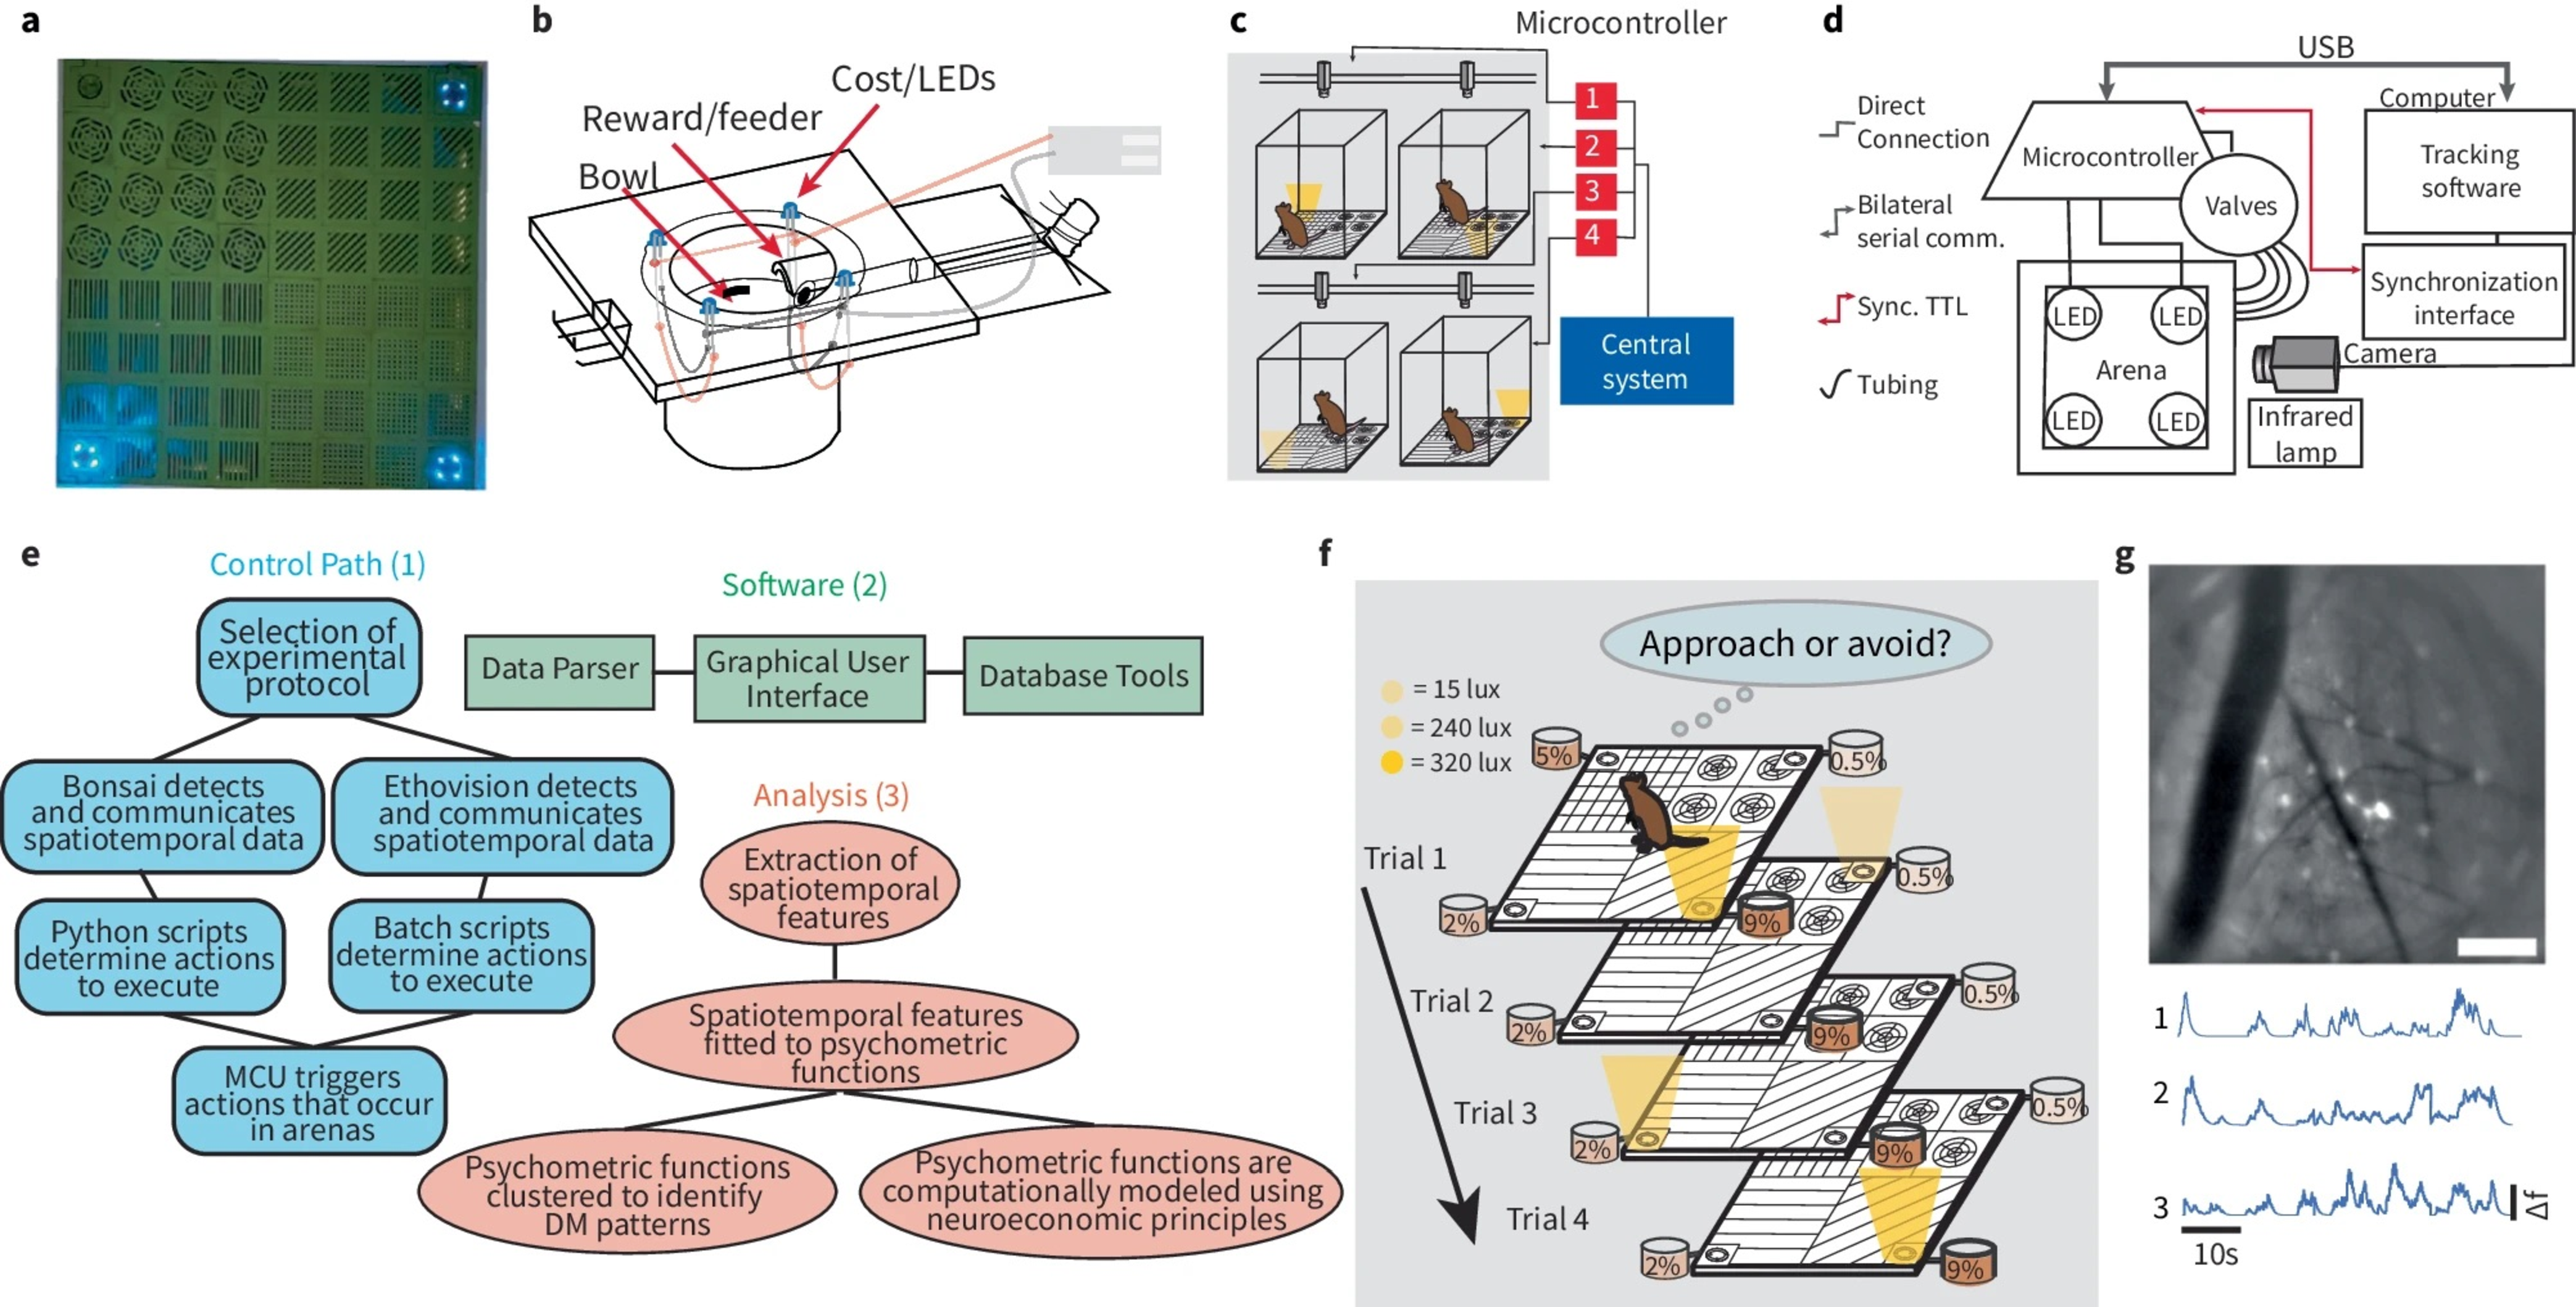
\includegraphics[width=\textwidth]{Figs/Record_main_1.pdf}
\end{figure}

\clearpage

\captionsetup{type=figure}  % Associate the following caption with the figure
\caption{\textbf{Modular and integrated system design.} (a) The maze floor is 3D-printed with four different patterns to 
distinguish the spatial locations of four bowls. Each bowl delivers a specific concentration of liquid reward. Four examples of LED light intensities are shown, from lowest to highest (upper left, moving clockwise). (b) Design of the feeders that deliver liquid rewards (e.g., sucrose at pre-determined concentrations) and cost (e.g., different light levels) via a ring of LEDs. Rewards are only dispensed if the animal’s location is detected to be close to the feeder (reward zone), meaning the animal must approach the illuminated LEDs to receive the sucrose solution. Light levels at each bowl can vary across trials and can be observed by the subject from a distance. (c) One microcontroller unit per maze (MCU; red boxes) allows each arena to run autonomously. Each MCU is connected to and communicates with one central system (blue box). This allows for flexibility in where the mazes are placed and increases the number of arenas that can be used concurrently. (d) Schematic of the complete maze set-up. Spatial information is collected through an infrared camera and used by NOLDUS or Bonsai to approximate an animal’s location and posture. The computer sets behavioral programs for each MCU. Data from the MCUs is sent to the computer and stored. (e) We developed three sets of software for RECORD. (1) Depending on which experiment was selected, either Bonsai or NOLDUS was used to detect spatial information. Custom Python or batch scripts determine what actions should be executed, sending that information to the MCU. The MCU then executes preprogrammed actions in the arenas (e.g., illuminate LEDs or dispense rewards). (2) Data collected from a session is sent to one of two custom parsers (which combine the trials and check for mismatches and consistency), depending on which experiment was run. The data can be accessed through a custom Graphical User Interface (GUI). Database tools were developed to expedite data retrieval and analysis. (3) Codes are used to extract features of behavior based on animal location, time, and choice. Using these features of animal behavior, we created modeling and analysis tools. We also developed synchronization scripts to allow our system to work with calcium imaging. (f) Cost–benefit Decision Making (decision-making) task. During each trial, the LEDs around one of the bowls are illuminated, signaling that the reward will be dispensed into that bowl. The reward at any spatial location is always the same (0.2–9\% sucrose). The animal decides whether to approach the port and consume the reward while being exposed to the LED light or avoid the bowl. The illuminated bowl is randomly determined for each trial. LED intensity varies from 15 to 320 lx and depends on the behavioral protocol. (g) Mean projection image of in vivo GCaMP8f fluorescence measured in the anterior dorsomedial striatum over the course of one behavior session. Bright-colored regions indicate cells exhibiting active calcium dynamics during the recorded session. Scale bar equals 100 $\mu$m. Calcium activity (df/f) trace of three example cells from the same session. The scale bar indicates 10 s.}
\label{fig:Record_main_1}

\vspace{1em}

The electronic setup combines custom and pre-existing software. During decision-making sessions, Bonsai or Noldus Ethovision software tracks each animal’s location (see the section “Methods: Spatial tracking for task execution”). Custom-developed programs use spatial information to execute trial events of a decision-making task. Since MCU output is task-dependent and RECORD generated ~1600 trials from ~40 rats run individually in one of eight arenas per day, we developed parsers; one parses only behavioral data while the other parses behavioral and calcium-activity data (see the section “Methods: Data preprocessing and storage”). We also developed a graphical user interface (GUI) that served as an easy-to-use front-end application for interacting with RECORD data (\hyperref[fig:Record_SI_1]{Supplemental Fig. 1d}). We scripted algorithms that extract spatiotemporal information (termed ‘behavioral features’) from each session for analysis/modeling. The features explored in this manuscript include approach time, approach rate, distance traveled, number of high-speed runs, number of rotations, number of stopping points, proportion of trials outside all reward zones, and reaction time (a description of each feature, their scripts, and scripts for features not used in this manuscript are provided in Methods: ‘Spatiotemporal behavioral dynamics’). All data analysis tools, modeling tools, and components used to build the RECORD system are listed in a “key resource table” (Table 2), with details provided in supplemental documents.

\vspace{1em}

Four main decision-making tasks were used for the initial validation of RECORD: reward/cost association, high-cost cost–benefit, low-cost cost–benefit, and alcohol trade-off. All tasks began with a tone signaling the start of a trial, followed by illumination of one feeder. Rats were given 6s to reach the reward zone. If the rat was within the reward zone (an ‘accept’ trial), the port remained illuminated while the reward was dispensed and consumed (typically 7 s, \hyperref[fig:Record_SI_1]{Supplemental Fig. 1e}). If the rat did not reach the reward zone (a ‘reject’ trial), the reward was not dispensed, and LEDs were turned off. The reward/cost association task was used to train rats to associate each reward level with a particular floor pattern (\hyperref[fig:Record_SI_1]{Supplemental Fig. 1f, g}). The high-cost cost–benefit task presented light intensities of 15 or 320 lx while low-cost tasks only had 15 lx trade-offs. On average, it took ~9 weeks for a rat to be trained for reward/cost association, low-cost cost–benefit, and high-cost cost–benefit tasks (\hyperref[fig:Record_SI_1]{Supplemental Fig. 1h}). To demonstrate that RECORD can be used in tandem with in vivo imaging systems, we implanted a GRIN lens and injected calcium indicator virus GCaMP8f into the anterior dorsomedial striatum (DMS), a region central to cost-benefit computations27 (see the section “Methods: Surgical procedures”) and measured calcium activity while the animals performed the low cost and high-cost cost–benefit tasks (\hyperref[fig:Record_main_1]{Fig. 1g} and \hyperref[fig:Record_SI_1]{Supplemental Fig. 1i, j}, see the section “Methods: Adaptable decision-making task batteries”).

\vspace{1em}

\noindent\textbf{Rats approach reward and avoid cost}\\
To establish how rats would respond to the cost and reward trade-offs presented by the RECORD system, we administered behavioral tasks where different sucrose concentrations (SC, 0.5\%, 2\%, 5\%, and 9\%; “reward”) were paired with LEDs of variable intensities (9, 10, 15, 20, 36, 42,160, 240, 260, 290 and 320 lx; “cost”). Unsurprisingly, rats approached reward/cost combinations more as SC increased (\hyperref[fig:Record_main_2]{Fig. 2a}, p $<$ 0.0001, \hyperref[fig:Record_SI_2]{Supplemental Fig. 2a}, for all statistics see ‘Statistics and Reproducibility’, Supplementary Note 6) and less as light intensity increased (\hyperref[fig:Record_main_2]{Fig. 2b}, p $<$ 0.0001, \hyperref[fig:Record_SI_2]{Supplemental Fig. 2b}). Analyzing approach rate along a spectrum of cost revealed context-dependent decision-making. The acceptance rate of rewards paired with 15 lx during sessions where only 15 lx was presented was ~80\%. The acceptance rate of rewards paired with 15 lx in sessions with interspersed trials of higher light intensities was significantly lower (p $<$ 0.0001, \hyperref[fig:Record_main_2]{Fig. 2c}).

\vspace{1em}

The spatiotemporal characteristics we term ‘behavioral features’ can be analyzed in several ways. Behavioral features can be examined by cost and reward level, an approach that shows some sex differences. Across all trials, females traveled further than males (p = 0.0025, \hyperref[fig:Record_main_2]{Fig. 2d}) while males had more high-speed runs than females (p = 0.0018, \hyperref[fig:Record_main_2]{Fig. 2e}); other features had no significant sex differences (\hyperref[fig:Record_main_2]{Fig. 2f-h}, \hyperref[fig:Record_SI_2]{Supplemental Fig. 2c-h}, see the section “Methods: Spatiotemporal behavioral dynamics”). Across both sexes, the number of high-speed runs increased with SC (p $<$ 0.0001, \hyperref[fig:Record_main_2]{Fig. 2e}) while both approach time (p = 0.0008, \hyperref[fig:Record_main_2]{Fig. 2f}) and proportion of trial outside all reward zones (p $<$ 0.0001, \hyperref[fig:Record_main_2]{Fig. 2g}) decreased as SC increased. Behavioral features were also compared across accept versus reject trials. Examining accept-only trials, females traveled further than males (p = 0.0038) and both sexes traveled less as SC increased (p = 0.0002, \hyperref[fig:Record_SI_2]{Supplemental Fig. 2i}). Also, during accept-only trials, both the number of stopping points (p = 0.0015, \hyperref[fig:Record_SI_2]{Supplemental Fig. 2j}) and number of high-speed runs (p $<$ 0.0001, \hyperref[fig:Record_SI_2]{Supplemental Fig. 2k}) increased as SC increased while the proportion of trial outside all reward zones decreased (p = 0.0003, \hyperref[fig:Record_SI_2]{Supplemental Fig. 2l}). During reject-only trials, distance traveled was the only feature significantly affected by SC (p = 0.046) and sex (p =0.014, \hyperref[fig:Record_SI_2]{Supplemental Fig. 2m}). Number of stopping points had no significance (\hyperref[fig:Record_SI_2]{Supplemental Fig. 2n}) while males ran more than females (p = 0.002, \hyperref[fig:Record_SI_2]{Supplemental Fig. 2o}). There were no significant interactions detected for proportion of trial outside all reward zones (\hyperref[fig:Record_SI_2]{Supplemental Fig. 2q}). Our data analysis tools allow behavioral features to be tracked across time within a trial or depicted in the spatial location where they were expressed (\hyperref[fig:Record_SI_2]{Supplemental Fig. 2q,r}).

\begin{figure}
  \centering
  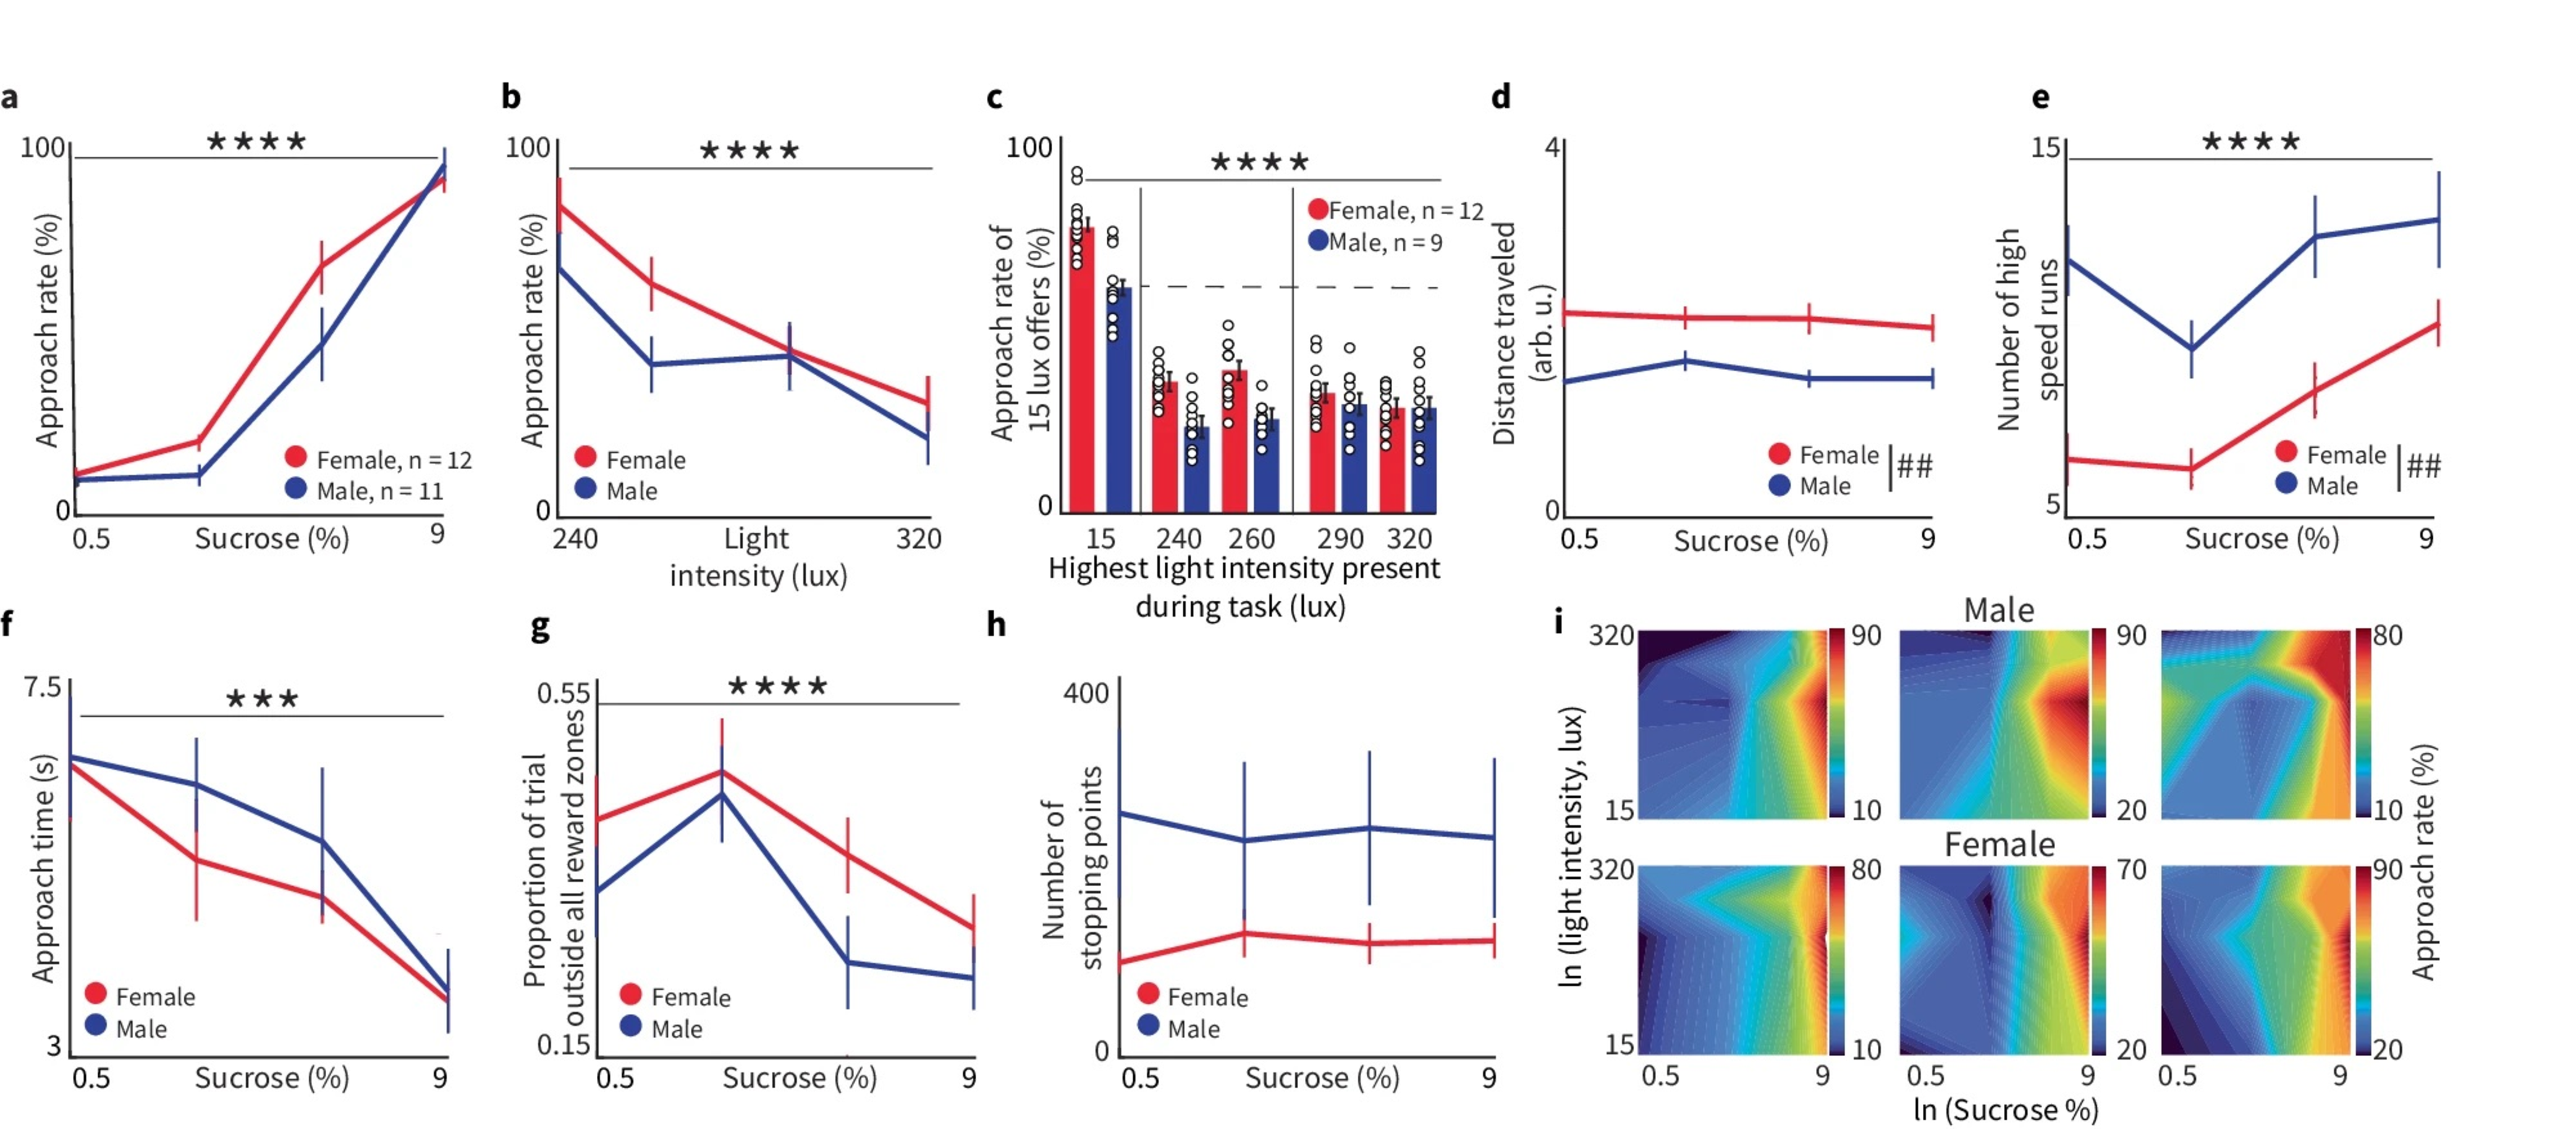
\includegraphics[width=\textwidth]{Figs/Record_main_2.pdf}
\end{figure}

\clearpage

\captionsetup{type=figure}  % Associate the following caption with the figure
\caption{\textbf{Validation of the RECORD system.} a Approach rates increase as the sucrose concentration (SC) increases. Both sexes approach the reward more as SC increases, indicated by a main effect of SC in the repeated measures ANOVA (ANOVARM, $****p < 0.0001$) and no main effect of sex (p = 0.06). Using 0.5–9\% sucrose yields sigmoidal psychometric functions. Error bars = mean ± SEM for all plots. Additional statistical analysis is reported in the section “Methods: Statistics and reproducibility”. * Is used to denote a significant effect of concentration ($*p \leq 0.05, **p \leq 0.01, ***p \leq 0.001, ****p \leq 0.0001$). b Approach rate decreases as light intensity increases (ANOVARM for light intensity $****p < 0.0001$). Sex had no significant effect on approach rate as light intensity increased (p = 0.153). c Bayesian analysis examining approach rate of 15 lx offers across sessions where different maximum light intensities were used. The effect of light intensity on approach rate was significant ($p < 0.0001$). While post-hoc analysis found significant sex differences at 15 lx (p = 0.0006), 240 lx (p = 0.0002), and 260 lx (p = 0.0002), there was no main effect of sex on approach (ANOVARM, p = 0.8). d–h Females and males demonstrate different patterns of time and movement dynamics between the initiation of a trial and when a choice is made. d Males travel shorter distances than females (ANOVARM, main effect of sex, \#\#p = 0.003) with no effect of SC (p = 0.089). e As SC increases, the number of high-speed runs increases (ANOVARM, main effect of SC, $****p < 0.0001$). Males had significantly more high-speed runs than females (ANOVARM, main effect of sex, \#\#p = 0.002). f Male and female rats enter the reward zone faster when higher SCs are offered (ANOVARM, main effect of SC, ***p = 0.0008) but there was no sex difference (ANOVARM, main effect of sex p = 0.4). g For both sexes (ANOVARM, main effect of sex: p = 0.233), rats spent less time in the center of the maze and more of the trial in a reward zone for higher SCs (ANOVARM, main effect of SC, $****p < 0.0001$). h Stopping points were unaffected by SC (p =0.98) or sex (p = 0.16). \# Is used to denote a significant effect of sex ($\# \leq 0.05, \#\# \leq 0.01, \#\#\# \leq 0.001, \#\#\#\# \leq 0.0001$ i Individual cross-benefit integration maps demonstrate that approach rates for individual subjects are not linearly related to cost and reward and are heterogeneous across individual subjects.}
\label{fig:Record_main_2}

\vspace{1em}

In summary, RECORD can generate cost-benefit maps displaying approach rates or behavioral features across multiple levels of rewards and costs. These can be averaged (\hyperref[fig:Record_main_2]{Fig. 2a-h}) or plotted for individuals, where the higher approach rates at higher light intensities suggest that for some rats, intense light may serve as a cue, rather than a deterrent, for the highest SCs, (\hyperref[fig:Record_main_2]{Fig. 2i}) and used to compare different experimental conditions.

\vspace{1em}

\noindent\textbf{Food deprivation alters decision-making}\\
Food deprivation (FD) may be used to motivate rodents to learn and perform decision-making tasks, but this itself may shift decision-making outcomes. RECORD functions without any form of deprivation, enabling comparisons of decision-making between FD and non-deprived conditions in a within-subject manner (see the section “Methods: Food deprivation alters decision-making”’). Approach rates increased after FD (\hyperref[fig:Record_main_3]{Fig. 3a}, p $<$ 0.0001) driven by increased approach for high-sucrose rewards (\hyperref[fig:Record_main_3]{Fig. 3a}, post hoc, 5\%: p $<$ 0.001, 9\%: p = 0.005). Rats who underwent FD accepted rewards more in low and high-cost conditions, regardless of sex (\hyperref[fig:Record_main_3]{Fig. 3b}).

\vspace{1em}

Approach time and proportion of time spent outside the reward zone were not impacted by FD (\hyperref[fig:Record_main_3]{Fig. 3c, d}) but other behavioral features were altered: rats stopped less often (p = 0.043), accelerated less (p = 0.025), and traveled further during sessions (p = 0.002, \hyperref[fig:Record_main_3]{Fig. 3e-g}) compared to ad libitum conditions. These patterns were mostly recapitulated when analyzing accept-only or reject-only trials (\hyperref[fig:Record_SI_3]{Supplemental Fig. 3a–h}). An averaged cost-benefit decision map demonstrates that approach rates were nearly linear across reward values (\hyperref[fig:Record_main_3]{Fig. 3i} vs. \hyperref[fig:Record_main_2]{Fig. 2i}), showing that FD induced robust insensitivity to cost (\hyperref[fig:Record_main_3]{Fig. 3i}, individual examples \hyperref[fig:Record_SI_3]{Supplemental Fig. 3n}).

\vspace{1em}

While the approach-enhancing impact of FD (Supplemental Fig. 5i, diet [ad libitum vs. FD]: female p = 0.0042, male p = 0.003) was observed in both sexes (\hyperref[fig:Record_SI_3]{Supplemental Fig. 3i}), FD altered sex differences for some behaviors. Sex differences in distance traveled were exacerbated by FD, while sex differences in the number of high-speed runs were decreased (\hyperref[fig:Record_SI_3]{Supplemental Fig. 3j-m}, interactions between sex and diet: distance traveled: p = 0.012, number of high-speed runs: p = 0.02). Sex differences in other measures were not impacted by FD.

\vspace{1em}

We explored how behavioral patterns are altered by FD by comparing cluster distributions of the parameterized psychometric functions between FD and ad libitum conditions (\hyperref[fig:Record_main_3]{Fig. 3j-m}, and \hyperref[fig:Record_SI_3]{Supplemental Fig. 3o-r}). There were subtle but significant shifts in cluster distribution (behavioral patterns) for distance traveled (\hyperref[fig:Record_main_3]{Fig. 3j}, Chi-square test, p = 0.0005). We compared individual changes in decision-making strategies across all features using radar plots (\hyperref[fig:Record_main_3]{Fig. 3k}, and \hyperref[fig:Record_SI_3]{Supplemental Fig. 3o, p}). We found behaviors to be significantly different between ad libitum fed and FD conditions by analyzing the difference in Euclidean distances between baseline and the two conditions (\hyperref[fig:Record_SI_3]{Supplemental Fig. 3l}, p $<$ 0.0001, two-sample Kolmogorov–Smirnov test and \hyperref[fig:Record_SI_3]{Supplemental Fig. 3q, r}, p $<$ 0.0001, p $<$ 0.0001). Finally, we examined FD-induced shifts in Euclidean distances within single individuals. The impact of FD was observed even in the distribution shift of Euclidean distances for an individual (\hyperref[fig:Record_SI_3]{Supplemental Fig. 3m}, p = 0.0006, Kolmogorov–Smirnov test). By comparing whether an experimental manipulation shifts the distribution for an individual, one could potentially characterize the extent to which the individual is resilient (no shift in distribution) or vulnerable (significant shift) to the manipulation.


\begin{figure}
  \centering
  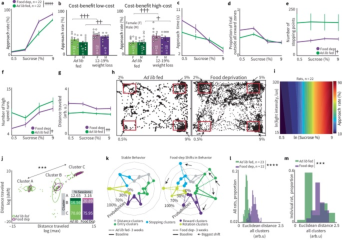
\includegraphics[width=\textwidth]{Figs/Record_main_3.pdf}
\end{figure}

\clearpage

\captionsetup{type=figure}  % Associate the following caption with the figure
\caption{\textbf{Food deprivation alters decision-making.} a While food-deprived, rats will approach higher SCs when compared to ad libitum fed sessions (main effect of deprivation, ANOVARM, ++++p = 0.0001, Tukey–Kramer honestly significant difference 5\%: p = 0.0005, 9\%: p = 0.0049). One rat developed a tumor during the alcohol task period and did not finish the full experiment, thus the incomplete data for that rat was not analyzed. + Is used to denote a significant effect of condition ($+ \leq 0.05, ++ \leq 0.01, +++ \leq 0.001, ++++ \leq 0.0001$. Error bars = mean ± SEM for all plots. b Food deprivation yielded a significant effect on both male and female for low cost (effect of condition, male **p = 0.0032, female ***p = 0.0009). In high-cost trials, approach rate was significantly different for both male and female groups (effect of condition, male *p = 0.0126, female ***p = 0.0004). c–g Food deprivation alters temporal and spatial aspects of behavior during decision-making. Approach times (c, p = 0.195) and proportion of trial spent outside of reward zones (d p = 0.12) were not significantly impacted by food deprivation. During food deprivation, stopping points decrease (e, ANOVARM +p = 0.04), rats had less high-speed runs (f ANOVARM +p = 0.02), and distance traveled during each trial is increased (g ANOVARM ++p = 0.0016). h Plots depicting an individual rat’s spatial location across a baseline and food deprivation session. Each point represents the location of the rat every 100 ms during the session. The rat moved more during a session under food deprivation (right) than ad libitum conditions (left). i During food deprivation, cross-benefit integration maps became homogenous straight lines and the non-linear relationship between reward and cost disappeared (n = 21: F = 12, M = 9). j Plot depicting cluster shifts between ad libitum fed and food deprived groups. Each data point represents two parameters for an individual session. We observed a significant difference in the count of sessions that belong to cluster A after food deprivation (chi-squared, ***p = 0.0005). Ellipses represent one standard deviation around cluster centroid. k Radar plots comparing ad libitum vs. food deprivation performance of individual rats vs. its baseline (“non-responder” on left plot, “responder” on right). Arrows point out the biggest visual differences between radar plots. l Using the average cluster distribution of ad libitum-fed rats, we created a distribution. We then calculated the Euclidean distance of each cluster of distance between ad libitum fed and food deprivation conditions and found that food deprivation shifted the peak completely outside of the baseline distribution. These shifts were statistically significant for both groups (****p < 0.0001, determined by two-sample Kolmogorov–Smirnov test). m Euclidian distances between individual rats for ad libitum fed and food deprivation conditions (***p = 0.0006, two-sample Kolmogorov–Smirnov test).}
\label{fig:Record_main_3}

\vspace{1em}

Collectively, our data demonstrate that FD non-specifically enhances the acceptance of cost-benefit tradeoffs by driving insensitivity to cost (\hyperref[fig:Record_main_3]{Fig. 3b, i}); FD also reshapes sex differences (\hyperref[fig:Record_SI_3]{Supplemental Fig. 3i-m}). Since RECORD does not require any deprivation, it avoids the impact, bias and alterations FD causes across decision-making and its associated behaviors.

\vspace{1em}

\noindent\textbf{Prior oxycodone usage impacts decision-making}
Given that opioid overdose deaths increased 14\% from 2020 to 2021, and that substance use impacts human decision-making\cite{bechara2005decision}, it is important to explore altered decision-making that accompanies substance use. To establish RECORD’s sensitivity to differences in decision-making before, during, and after opioid administration, we conducted an experiment examining how oxycodone self-administration and abstinence impact decision-making. Rats were trained on the low-cost cost–benefit task and then exposed to a 14-day period of oxycodone self-administration in an operant chamber (see the section “Methods: Oxycodone self-administration and abstinence”). On average, rats self-administered 3.99 mg/session. Consistent with other studies\cite{zanni2020female}, females administered roughly twice as much oxycodone as males (females: 5.6 mg/session; males: 2.7 mg/session). Three to four hours after self-administration, rats ran a RECORD cost-benefit task (see the section “Methods: Oxycodone behavioral task”). After the self-administration period, rats entered forced abstinence where they continued to perform the RECORD task. Throughout, their performance was compared to the control group of rats who trained and performed RECORD tasks without any manipulations (\hyperref[fig:Record_main_2]{Fig. 2}).

\vspace{1em}

During 14 days of oxycodone self-administration, the relationship between SC and approach rate flattened (\hyperref[fig:Record_main_4]{Fig. 4a}, p = 0.1051 ANOVA, p = 0.005 KS test). This hyposensitivity to reward magnitude during opioid administration is consistent with several other studies36,37,38. When comparing task performance during the 14 days of self-administration to that of the control group, no other behavioral feature differed between the two groups (\hyperref[fig:Record_main_4]{Fig. 4b-f}). After 30 days of abstinence, the approach rate remained flattened compared to the control condition (\hyperref[fig:Record_main_4]{Fig. 4g}, p = 0.019), suggesting a persistent reward hyposensitivity across reward levels. Amongst other behavioral features, only the distance traveled differed between the two groups after abstinence (\hyperref[fig:Record_main_4]{Fig. 4h-l}, p = 0.045). These data might suggest a limited impact of oxycodone use on decision-making behavior; however, a different picture emerges when sex is considered.

\vspace{1em}

There were reduced sex differences in approach rate (\hyperref[fig:Record_main_4]{Fig. 4m}, p = 0.04, Sex × Concentration interaction; p $>$ 0.05 for all post-hoc comparisons between Female-oxy and Male-oxy) but not for approach times (\hyperref[fig:Record_SI_4]{Supplemental Fig. 4a}). Importantly, sex differences in other behavioral features were impacted by oxycodone. For example, oxycodone self-administration increased the distance traveled by males but decreased the distance traveled by females (\hyperref[fig:Record_main_4]{Fig. 4n}, Sex × Condition interaction, p $<$ 0.0001). Similarly, these opposing effects were observed for the number of high-speed runs (\hyperref[fig:Record_main_4]{Fig. 4o}), time spent in reward zones, and number of stopping points (\hyperref[fig:Record_SI_4]{Supplemental Fig. 4b, c}). Collectively, oxycodone self-administration impacts decision-making behavior within sex, and altered sex differences in cost-benefit decision-making.

\vspace{1em}

Many sex differences in behavioral features returned to pre-oxycodone levels after 30 days of abstinence, including approach rate (\hyperref[fig:Record_main_4]{Fig. 4}p, Sex × Condition interaction, p = 0.65). Distance traveled was the only behavioral feature to show perturbed sex differences after 30 days of abstinence (\hyperref[fig:Record_main_4]{Fig. 4}q, Sex × Condition interaction, p = 0.0165). All other features returned to pre-oxycodone levels including high-speed runs (\hyperref[fig:Record_main_4]{Fig. 4}r), approach time, proportion of trial spent outside feeder zones, and number of stopping points (\hyperref[fig:Record_SI_4]{Supplemental Fig. 4}d–f).

\vspace{1em}

During oxycodone self-administration, the percentage of sessions that displayed sigmoidal functions relating approach rate to reward levels was reduced to ~40\%. After 30 days of abstinence from oxycodone, we found that the percentage of sessions with approach rate sigmoidal functions increased to ~55\%, which was still significantly below the pre-drug levels of ~95\% (\hyperref[fig:Record_main_4]{Fig. 4}s). When comparing sigmoid session frequency across individual rats, we found that all rats were impacted by oxycodone self-administration, but there was significant inter-individual variation (\hyperref[fig:Record_SI_4]{Supplemental Fig. 4}g). A significant correlation between the amount of oxycodone self-administered and the percentage of sessions that generate sigmoid shaped functions suggests that greater oxycodone consumption leads to the decreased percentage of sigmoidal functions used to relate costs to rewards (\hyperref[fig:Record_SI_4]{Supplemental Fig. 4}h).

\vspace{1em}

\begin{figure}
  \centering
  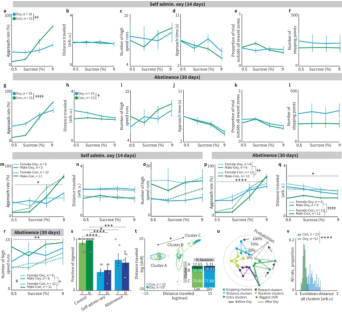
\includegraphics[width=\textwidth]{Figs/Record_main_4.pdf}
  \label{fig:Record_main_4}
\end{figure}

\clearpage

\captionsetup{font = scriptsize, type=figure}  % Associate the following caption with the 
\begin{singlespace}
\noindent Figure 4.\textbf{Decision-making with substance use: Oxycodone} a–f Behavioral features compared between the control and oxycodone conditions during the 14 days of self-administration. Two rats (one male and one female) were incapable of running behavioral sessions after cocaine self-administration, and thus, their behavioral data were not collected. a Approach time was flattened during oxycodone self-administration (++p = 0.0049, Kolmogorov–Smirnov test), while the other features demonstrated no significant differences between conditions (b distance traveled: p = 0.9132, c number of high-speed runs: p = 0.97, d approach times: p = 0.26, e proportion of trial outside all reward zones: p = 0.75, f number of stopping points: p = 0.5). Error bars = mean ± SEM for all plots. g–l Behavioral features compared between the control and oxycodone conditions after 30 days of abstinence. g Approach time remained significantly different (+p = 0.0187) from the control condition. h Rats traveled significantly further after 30 days of abstinence from oxycodone (+p = 0.045). All other features remained were not different between groups (i, number of high-speed runs: p = 0.44, j approach time: p = 0.74, k proportion of trials outside all reward zone: p = 0.32, l number of stopping points: p = 0.17). m Oxycodone self-administration produced a unique set of sex differences in decision-making that differed from those observed in the control group (p = 0.17, Sex × Condition interaction, *p = 0.04, Sex × Concentration interaction). One male and one female rat were incapacitated throughout oxycodone self-administration and were unable to perform behavioral sessions. n, o While the magnitude of sex differences was not impacted by oxycodone self-administration, males became more female-like and vice versa for two behavioral features. n Whereas oxycodone increased the distance traveled for males, it decreased the distance traveled for females (p < 0.0001, Sex × Condition interaction). o Similarly, oxycodone increased the high-speed runs for females, while decreasing them for males (p < 0.0001, Sex × Condition interaction). p–r After 30 days of abstinence, behavioral features altered by oxycodone shift towards pre-oxycodone values for both males and females but remain impacted by prior self-administration. The approach rate remained significantly different between the OXY and CON conditions (p, main effect of condition, ++p = 0.0016; Condition × Sucrose Concentration interaction, ****p < 0.0001). No sex differences were observed in the Oxy group for any reward level (post-hoc, p < 0.08 for all points). q For females, the distance traveled returned to pre-oxycodone levels, but males still showed significantly greater distance traveled during abstinence (p = 0.4449 and p = 0.0093, respectively, Sex × Condition interaction, p = 0.0165, n-way ANOVARM). Concentration (****p < 0.0001) and condition (++++p < 0.0001) effects were significant. r In contrast, the number of high-speed runs returned to pre-oxycodone levels for both sexes (**p = 0.0057 effect of concentration, p = 0.0853 effect of oxycodone, p = 0.0506 effect of sex, and p = 0.2045 Sex × condition interaction, n-way ANOVARM). s After analyzing the frequency of sigmoidal data for the approach rate measure, we found that oxycodone significantly reduced the percent of the session with sigmoidal psychometric functions (CON ~90\% vs. Self-admin ~40\%; one-way ANOVAs: female CON vs. female Self-admin and male CON vs. male Self-admin, ****p < 0.0001). After 30 days of abstinence from oxycodone, sigmoid frequency recovered to ~55\% but was still significantly lower than the levels observed in controls (female CON vs. female Abstinence, p = 0.01; male CON vs. male Abstinence, ***p = 0.0003). t Plot depicting “macro-migration" between control and oxycodone groups. Each data point represents a fitting parameter for an individual session. We detected a significant population migration away from cluster A after oxycodone self-administration (chi-squared p = 0.0235). Ellipses represent one standard deviation around the cluster centroid. u Radar plot comparing baseline and abstinence conditions of a “responder” rat’s behavioral clusters. A ‘responder’ was defined as an individual with a significant shift in Euclidian distances after oxycodone task performance. Arrows indicate the clusters within each behavioral feature that are shifted. v Using the average cluster distribution of baseline rats, we created a normal distribution. We then calculated the Euclidean distance of each cluster of the distance between baseline and oxy conditions and found that oxycodone shifted the peak completely outside of the baseline normal distribution. This shift in the Euclidean distance of oxycodone cluster distributions was statistically significant (****p < 0.0001, determined by the two-sample Kolmogorov–Smirnov test).
\end{singlespace}


% \captionsetup{labelsep=period, font={small, singlespacing}}  % Reset to desired settings
\captionsetup{labelsep=period, font={small, singlespacing}, type=figure}

\vspace{1em}

Radar plots and Euclidean distance analysis provide insight into behavioral shifts after oxycodone self-administration (\hyperref[fig:Record_main_4]{Fig. 4}t–v). Distance traveled had significant shifts in preferred clusters (behavioral patterns) when compared to baseline clusters (\hyperref[fig:Record_main_4]{Fig. 4}t, p = 0.0235, p = 0.9455 and p = 0.1187 for clusters left, middle, and right, chi-square test). Calculating the average psychometric function for each cluster within the oxycodone and baseline groups (\hyperref[fig:Record_SI_4]{Supplemental Fig. 4}i), we identified three distinct ways that distance traveled relates to reward values. Euclidean distances were significantly different after oxycodone use (\hyperref[fig:Record_main_4]{Fig. 4}v, p $<$ 0.0001, Kolmogorov–Smirnov), demonstrating significant changes to behavioral patterns. Individual radar plots comparing baseline cluster probabilities to the last week of oxycodone self-administration (\hyperref[fig:Record_main_4]{Fig. 4}u, \hyperref[fig:Record_SI_4]{Supplemental Fig. 4}j, k) depict behavioral shifts. Finally, oxycodone dramatically increased individual Euclidean distances between the rat’s baseline and abstinence periods (\hyperref[fig:Record_SI_4]{Supplemental Fig. 4}l, p = 0.001, Kolmogorov–Smirnov). These analyses reveal that the “average” psychometric function (e.g. \hyperref[fig:Record_main_4]{Fig. 4}a) may not be representative of individual behavioral strategies (\hyperref[fig:Record_main_4]{Fig. 4}t). This failure of averaging has been previously described for neuronal responses39,40 but is underappreciated in behavioral contexts.

\vspace{1em}

\noindent\textbf{Sucrose alcohol trade-off}
To further showcase the versatility of RECORD, we created a task to probe alcohol as a cost/reward. We developed a version of our decision-making task where alcohol was mixed with sucrose solutions to yield four trade-off solutions with inverse concentrations of the two substances: 0.5\% sucrose and 20\% alcohol, 2\% sucrose and 10\% alcohol, 5\% sucrose and 2\% alcohol, and 9\% sucrose and 0.5\% alcohol (\hyperref[fig:Record_main_5]{Fig. 5}a, see the section “Methods: Sucrose vs. alcohol trade-off”).

\vspace{1em}

Analyzing behavioral features between control and different stages of task performance revealed limited interactions. Approach rate during the first three weeks of task performance demonstrated that rats approached higher SCs more than the lower SCs, as expected. However, despite the aversive properties of ethanol\cite{pautassi2011ethanol, anderson2010ethanol}, the approach rate was significantly higher for the alcohol task compared to the control group (\hyperref[fig:Record_main_5]{Fig. 5}b, Condition × Concentration, p = 0.003). After nine weeks of task performance, females exhibited higher approach rates than males (\hyperref[fig:Record_main_5]{Fig. 5}c, Sex × Concentration, p = 0.044). All other features had no significant interactions across initial-late task performance (\hyperref[fig:Record_main_5]{Fig. 5}d–i).

\vspace{1em}

Unlike oxycodone self-administration, alcohol exposure did not alter the proportion of sessions with sigmoidal psychometric functions (\hyperref[fig:Record_main_5]{Fig. 5}j). However, like oxycodone, the percentage of sessions distributed across clusters varied greatly between the control and alcohol task (\hyperref[fig:Record_main_5]{Fig. 5}k, p = 0.0232, p = 0.1753, and p = 0.0003 for clusters left, middle, and right respectively, chi square test). Radar plots of individual rats with no, moderate and strong differences between initial and late alcohol task performance show how behavioral strategies are differentially shifted across individuals (\hyperref[fig:Record_main_5]{Fig. 5}l–n). Euclidean distances for the population (\hyperref[fig:Record_main_5]{Fig. 5}o, p $<$ 0.0001) and an example of an individual rat (\hyperref[fig:Record_main_5]{Fig. 5}p, p = 0.001) demonstrate significant changes in decision-making behavior. This type of analysis may enable the identification of resilient or vulnerable subjects, depending on their Euclidean distances before and after substance use/other experimental conditions.

\begin{figure}
  \centering
  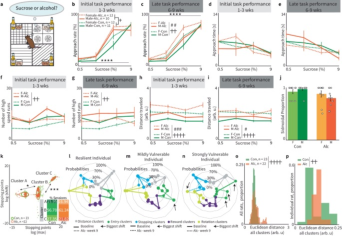
\includegraphics[width=\textwidth]{Figs/Record_main_5.pdf}
  \label{fig:Record_main_5}
\end{figure}

\clearpage

\begin{singlespace}
    \noindent Figure 5.\textbf{Alcohol decision-making.} a During the alcohol task, rats were presented with a trade-off between sucrose and ethyl alcohol. 0.5\% sucrose was delivered in 20\% alcohol, 2\% was delivered in 10\% alcohol, 5\% was delivered in 2\% alcohol, and 9\% was delivered in 0.5\% alcohol. Outside of this change in reward offered, the task operated similarly to the high-cost and low-cost cost-benefit tasks. We examined how exposure to alcohol during task performance affects decision-making over time (9 weeks) relative to rats running on the version of the task without alcohol (Fig. 2). b When initially performing the alcohol trade-off task, male and female rats maintained preferential acceptance of offers with 5\% and 9\% sucrose while rejecting 0.5\% and 2\% sucrose (main effect of SC, ****p < 0.0001) with no sex differences (sex, p = 0.4). However, alcohol-exposed rats had significantly increased approach rates (main effect of task type, +p = 0.0178; group × SC interaction, p = 0.0025). Error bars = mean ± SEM for all plots. c After nine weeks of task performance, all three main effects were significant (sex \#\#p = 0.0015, condition ++p = 0.01, concentration ****p < 0.0001, n-way ANOVARM). The interaction between sex and SC was also significant with females accepting more than males and the control group overall (p = 0.044, n-way ANOVARM). Females approached significantly more than males (p = 0.03) when taking both initial and late alcohol task performance groups into consideration. d Approach time tracked during the initial (first 3 weeks) task performance had an overall significant main effect of concentration (p < 0.0001), but no other significant interactions when compared to the control group (sex × condition: p = 0.254, sex × concentration: p = 0.2729, task type × concentration: p = 0.7127) or main effects (sex = 0.9775, task type = 0.4457). e Approach time after prolonged (6–9 weeks) alcohol trade-off task performance continued to have no significant main effects or interactions when compared to the control group. However, there was still a significant response to concentration among the alcohol group (p < 0.0001). f and g For both initial and late task performance, the number of high-speed runs had no significant interactions for sucrose concentration or sex within alcohol groups. However, we detected a significant effect of the condition when comparing alcohol and control groups (f ++p = 0.0028, g ++p = 0.0031), as well as a significant effect of sex (f p = 0.0003, g p < 0.0001). h and i Distance traveled during both initial (\#\#\#p = 0.0004) and late (\#p = 0.045, ANOVARM) task performance was significantly different between sexes, with females traveling further than males, with an overall effect of condition (++++p < 0.0001). There were no significant interactions while comparing initial or late task performance to the control group. j The alcohol trade-off task did not significantly impact sigmoid frequency, which we defined as the proportion of sessions where approach rate formed sigmoid-shaped data as opposed to parabolic or undefined data (one-way ANOVA male control n = 10 vs. male alcohol n = 10, p = 0.36, female control n = 12 vs. female alcohol n = 10, p = 0.08). k Plot depicting “macro-migration" between control and alcohol groups. Each data point represents a fitting parameter for an individual session. We detected a significant population migration in clusters A (p = 0.0232) and C (p = 0.0003) compared to control group clusters (n = 20, M = 10, F = 10). Ellipses represent one standard deviation around cluster centroid. l–n Examples of radar plots comparing baseline and alcohol conditions of the behavioral cluster of three individual rats who had increasing differences in Euclidean distances before and after alcohol trade-off task performance. Some rats maintained consistent cluster probabilities (e.g., left, low), some rats had moderate shifts in cluster probabilities (middle), and other rats had high differences between cluster probabilities measured using Euclidean distances. Arrow indicates a large shift. o Using the average cluster distribution of baseline rats, we created a distribution. We then calculated the Euclidean distance of each cluster of distance between baseline and alcohol conditions and found that alcohol shifted the peak completely outside of the baseline distribution. These shifts were statistically significant for both groups (****p < 0.0001, determined by two-sample Kolmogorov–Smirnov test). p Euclidian distances between clusters for baseline and alcohol trade-off conditions (**p = 0.0011, two-sample Kolmogorov–Smirnov test).
\end{singlespace}

% \captionsetup{labelsep=period, font={small, singlespacing}, type=figure}

\clearpage

\subsubsection{Discussion}
RECORD combines custom-designed hardware and software, providing a customizable tool that quantifies decision-making and behavioral correlates across experimental conditions. RECORD is an automated system that can identify deviations in decision-making and behavior for sub-groups and individuals. Multiple levels of rewards and costs enable thorough comparisons of decision-making between sessions, conditions, contexts, and across time. RECORD’s utility is enhanced by its adaptability and by implementing task series that progressively change one variable to isolate components of decision-making.

\vspace{1em}

RECORD is a comprehensive behavioral system that does not implement food deprivation or water restriction to train rats for behavioral protocol performance. Food and water restriction alters behavior and task performance\cite{goltstein2018food} (\hyperref[fig:Record_main_3]{Fig. 3}) along with reducing the detectability of sex differences in decision-making (\hyperref[fig:Record_SI_3]{Supplemental Fig. 3}i–m). This is suboptimal since animal paradigms that limit sex differences are less conducive to developing meaningful clinical interventions\cite{clayton2016studying, legates2019sex}. Generally, sex differences observed using RECORD tends to align with prior behavioral research, like female rats approaching alcohol more than males\cite{juarez1999sex}, however there remain several questions to explore with the RECORD system including exploring sex differences during risky, probabilistic, or intertemporal decision-making in a foraging-like framework.

\vspace{1em}

Another strength of RECORD is its’ sensitivity to detect behavioral differences, conferred by using multiple levels of reward and cost within each subject. For example, if an experiment used a different decision-making task with only rewards valued above 2\% sucrose, one might erroneously conclude that oxycodone abstinence does not impact decision-making task performance (\hyperref[fig:Record_main_4]{Fig. 4}g). Our data reveal heterogeneity across individuals in how oxycodone self-administration and its abstinence impact decision-making (\hyperref[fig:Record_main_4]{Fig. 4}s–v, \hyperref[fig:Record_SI_4]{Supplemental Fig. 4}g, h), making RECORD a powerful tool to study disorders.

\vspace{1em}

RECORD’s foraging-like environment establishes a framework for studying ecologically relevant decision-making with high experimental control. The tone signaling trial initiation is unnatural, other aspects of naturalistic rodent behavior are included, like free movement, identification of reward locations using visual/tactile cues, and determining whether foraging is worthwhile\cite{juavinett2018decision}. This may contribute to the animals’ willingness to perform the task without food/water deprivation. Future experiments could implement natural auditory cues\cite{juavinett2018decision} or burrows underneath the arena. An additional factor often present in nature is ambiguity. Tasks could incorporate ambiguity by (1) using multiple tones to signal trial onset, but different tones for differing probabilities of reward dispensation, (2) comparing bowls that deliver a particular concentration of sucrose with high-probability to bowls that deliver the same sucrose concentration with low-probability, or (3) randomize session lengths. Since RECORD is modular, multiple connected arenas would allow rats to access different trade-offs depending on where they explore.

For more thorough behavioral analysis, RECORD could be used with B-SOiD, a software that provides measures of individual limb movements to delineate decision-making states or clusters more definitively\cite{hsu2021b}. Along with B-SOiD, RECORD could be used with behavioral software tools like A-SOiD\cite{tillmann2024soid}, DeepLabCut\cite{mathis2018deeplabcut, nath2019using, monsees2022estimation, lauer2022multi}, SLEAP\cite{pereira2022sleap}, and BehaviorDEPOT\cite{gabriel2022behaviordepot}, to investigate behavioral and decision-making links in various experimental setups. Overall, RECORD is a versatile tool that is capable of a wide array of decision-making experiments, providing a foundation for the thorough analysis of both decision-making and its associated behaviors.

\clearpage

\subsubsection{Methods}
\noindent\textbf{Animal ethics statement}\\
The project received approval for all protocols from the University of Texas at El Paso Institutional Animal Care and Use Committee and followed the Guide for Care and Use of Laboratory Animals (IACUC reference number: A-202009-1).

\vspace{1em}

\noindent\textbf{RECORD system overview}\\
In this paper, we outline a novel and customizable behavioral system designed to study decision-making in rodents, the Reward-Cost in Rodent Decision-making (RECORD) system. RECORD synergistically utilizes (1) 3D-printed arenas, (2) microcontroller-driven electronics, (3) camera-based animal tracking, (4) data acquisition software, (5) custom parsing software, (6) databasing software, and (7) analysis software. This system is high throughput while being sufficiently sensitive for the identification and quantification of sub-group/individual decision-making behaviors. The RECORD system can be used either alone or in conjunction with third-party hardware/software for the acquisition of other measures, such as neuronal recordings. Herein, assembly instructions, components used, suggested dimensions, and links to all pertinent GitHub repositories are provided.

\vspace{1em}

\noindent\textbf{Cost and reward}\\
During cost/benefit conflict tasks, variable light intensities were used as aversive stimuli while sucrose solutions were used as rewarding stimuli. Blue (~470 nm wavelength) high-intensity light-emitting diodes (LEDs) were used since this color of light has been established as being aversive to rats\cite{friedman2017chronic, friedman2020striosomes, friedman2015corticostriatal}. Light also cued which feeder would dispense a reward for each trial. Each feeder was fitted with an assembly of four LEDs connected in parallel, forming a ring around the feeder bowl. Varying concentrations of sugar diluted in water (sucrose solution, see ‘Adaptable decision-making task batteries’), were deposited into the bowl of a feeder piece. For alcohol tasks, different concentrations of ethanol were mixed with sucrose solutions (see the section “Sucrose vs. alcohol trade-off”).

\vspace{1em}

\noindent\textbf{Food deprivation alters decision-making}\\
Aberrant decision-making and behavioral changes were assessed in each rat through the implementation of a food deprivation paradigm. While running cost/benefit conflict tasks, rats were waned off their regular meals and weighed daily. Rats were initially given 20\% of their body weight in daily food, then food availability was gradually reduced to only 5 g per rat per day over the course of three weeks. For each rat, every session was categorized in one of two ways: one where a weight reduction of 0-10\% of their initial weight was observed, and another where a 10-20\% weight reduction was observed. Food deprivation was halted after rats had lost around 20\% of their pre-food deprivation weight, which occurred after about 3 weeks.

\vspace{1em}

\noindent\textbf{Sucrose vs. alcohol trade-off}\\
Animals ran high- and low-cost cost–benefit tasks for 9 weeks where cost levels presented during the task were rotated between level 1 (low-cost) only, level 1/level 3, and level 3 only (high-cost) five days a week. Animals were subjected to a sucrose vs. alcohol trade-off task based on the same cost-benefit tasks where different concentrations of alcohol were added to the existing levels of sucrose solutions. The amount of alcohol per solution increased as sugar concentration decreased (9\% sucrose + 1\% alcohol, 5\% sucrose + 4\% alcohol, 2\% + 10\% alcohol, and 0.5\% sucrose + 20\% alcohol).

\vspace{1em}

\noindent\textbf{Oxycodone self-administration and abstinence}\\
The self-administration task is based on one used in multiple published experiments\cite{moschak2021opposing, moschak2018low, moschak2021sex, moschak2017impulsive, moschak2018neuronal, bossert2020rat, altshuler2021role}. Mildly water-deprived rats self-administered either oxycodone or water reward (with yoked saline) 6 h/day for 14 days, as described previously\cite{friedman2017chronic}. During each trial of the task, a nosepoke aperture was illuminated. Nosepokes into the illuminated aperture resulted in a bolus of oxycodone (0.05 mg/kg/infusion) or water/yoked saline (volume matched) coupled with a 20 s tone/house light stimulus. During the 20 s tone/house light stimulus, the nosepoke aperture was darkened and further nosepokes were recorded but did not result in drug delivery. Animals were also tested on extinction of self-administration both 1 day and 30 days following cessation of self-administration; this paradigm was sufficient to induce an ‘incubation of craving’ for oxycodone, that is, an increase in drug-seeking behavior at 30 days\cite{friedman2020striosomes}. During extinction, nosepokes resulted in tone/house light stimulus, but no oxycodone or water/yoked saline.

\vspace{1em}

\noindent\textbf{Oxycodone behavioral task}\\
During RECORD behavioral sessions, rats performed a slightly modified version of the cost/benefit association task with the same rewards being dispensed, however only 280 lx was used as a cost as opposed to varying light intensities. This modification to the protocol was made due to a perceived hypersensitivity to the cost light, which we believed was due to the introduction of oxycodone. Additionally, we found that during self-administration and abstinence, some rats became increasingly aggressive toward experimenters and spent a large amount of time biting at the arena components instead of participating in the trial. These rats (n = 2) were removed from the study entirely.

\vspace{1em}

\noindent\textbf{Spatiotemporal behavioral dynamics}\\
To analyze individual decision-making strategies, a set of “features” were defined and extracted from data generated during behavioral trials (e.g., speed, orientation, position, etc.). After analysis, these features were recorded and stored in the PostgreSQL database in a separate table, then a psychometric function was plotted, with all four levels of reward along the x-axis and the feature tracked along the y-axis. The following is a list of the features extracted along with a definition of each one (\hyperref[fig:Record_main_1]{Fig. 1}e).

\vspace{1em}

\begin{enumerate}
    \item \textit{Distance traveled}: Overall Euclidean distance traveled by the animal in the normalized trajectory (\url{https://github.com/atanugiri/Feature-Extraction/tree/main/Run%20Time}), i.e. the two-dimensional plane created by the arena floor normalized to the camera’s field of view.
    \item \textit{Travel pixel}: The number of pixels that were traveled by the animal between trial start and trial end in the normalized trajectory (\url{https://github.com/atanugiri/Feature-Extraction/tree/main/Trajectory%20Plots, https://github.com/atanugiri/Feature-Extraction/tree/main/Run%20Time}). 
    \item \textit{Proportion of high-speed runs (bigaccelerationperunittravel)}: The total number of outliers present in a set of acceleration measurements. We calculated this based on the median and the standard deviation of the acceleration data divided by the distance traveled (\url{https://github.com/atanugiri/Feature-Extraction/tree/main/Acceleration%20and%20Jerk%20Outliers}).
    \item \textit{Stopping points}: Defined as the number of times the rat comes to a complete stop (moves $<$ 0.1 units in both X and Y direction within a 3-s window) during the trial (\url{https://github.com/atanugiri/Feature-Extraction/tree/main/Stop%20Time}).
    \item \textit{Rotation points}: Defined as the number of rotations performed by the animal during each trial. A vector was defined from the center point of the rat to the head of the rat. Angular changes $>180^\circ$ in the vector within a 1.5 s window were defined as one rotation (\url{https://github.com/atanugiri/Feature-Extraction/tree/main/Rotation%20Points}).
    \item \textit{Approach time}: Refers to the time it takes the animal to reach an offer location after the “trial start” tone is presented (\url{https://github.com/atanugiri/Feature-Extraction/tree/main/Run%20Time}).
    \item \textit{Proportion of trial outside all reward zones}: Time the animal spent in the center of the arena divided by the number of trials in a session (\url{https://github.com/atanugiri/Feature-Extraction/tree/main/Passing%20Central%20Zone}).
\end{enumerate}

All Matlab codes used for this analysis are available in the “feature extraction” Github repository (\url{https://github.com/atanugiri/Feature-Extraction}). Within the different functions used to extract each feature can be found.

\clearpage

\subsubsection{Statistics and reproducibility}
A repeated measures analysis of variance (ANOVA) was conducted using the MATLAB ranova function to examine the effects of within-subject factors, such as sucrose concentration, and between-subject factors, including Sex and experimental conditions (control vs food deprivation). Additionally, pair-wise comparisons were conducted to further explore the differences between groups using a post-hoc analysis, specifically Tukey’s honestly significant difference method, implemented with the MATLAB multcompare function. To assess the between-subjects differences, a two-sample Kolmogorov-Smirnov test was also employed with the MATLAB kstest2 function. Three-way ANOVA was used to investigate the main effects of each of the three factors (e.g., sucrose concentration, sex, treatment groups) and any potential interactions between them.

The scripts for statistical analysis are located in our Github repository: \url{https://GitHub.com/atanugiri/Data-Analysis/tree/main/Statistics}.

\clearpage

\subsubsection{Data availability}
Database links go here All data used to produce the figures presented, including raw Excel Ethovision output, PostgreSQL database backups, and CSV data, are provided on the Harvard Dataverse\cite{ibanez2024record}: \url{https://doi.org/10.7910/DVN/QADUKS}.

\vspace{1em}

\subsubsection{Code availability}
Features for data analysis are contained in our ‘Feature Extraction’ repository (\url{https://GitHub.com/atanugiri/Feature-Extraction})

\clearpage

\subsubsection{Supplementary information}

% Supplementary figure on one page
\begin{suppfigure}[htbp]
  \centering
  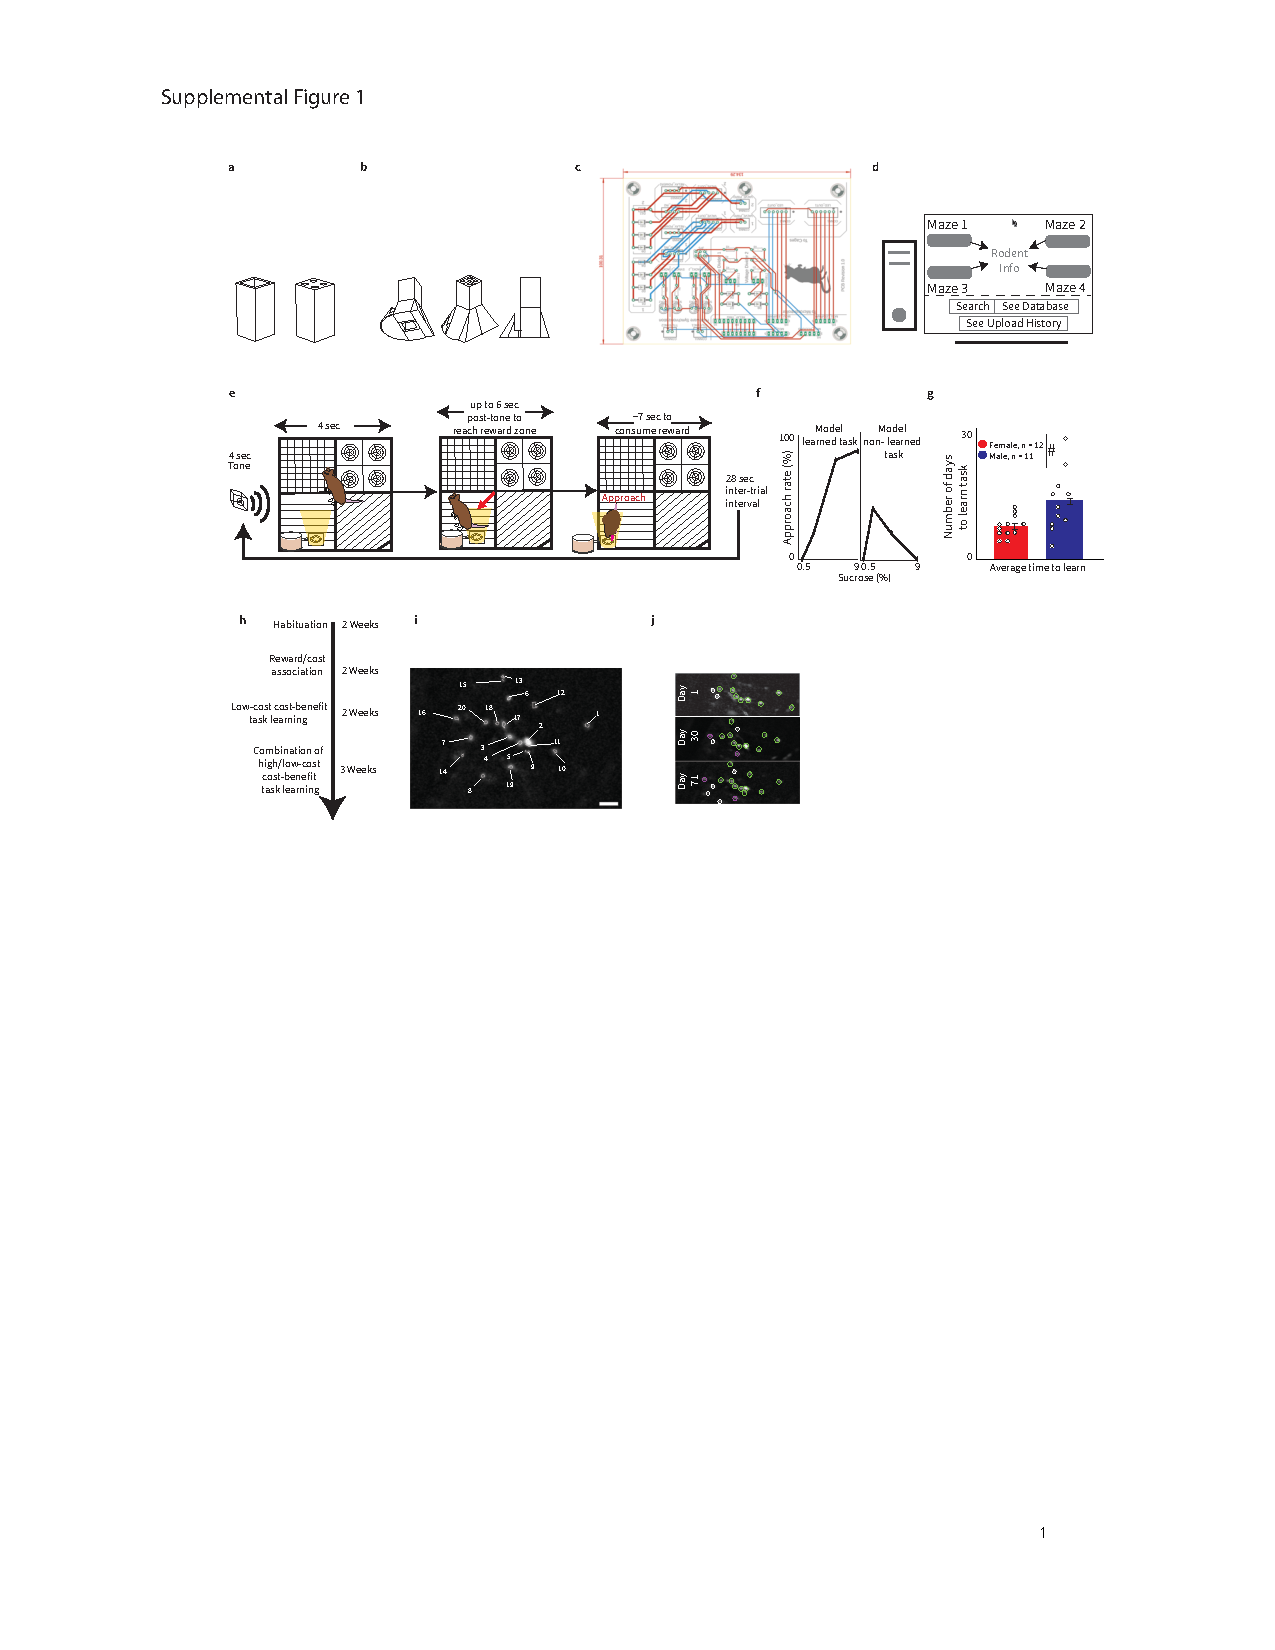
\includegraphics[width=\textwidth]{Figs/Record_SI_1.pdf}
  % No caption here
  \label{fig:Record_SI_1}
\end{suppfigure}

\clearpage  % Move to the next page for the caption

\begin{singlespace}
\noindent Figure S1. \textbf{System Components and Task Training} a. 3D-printed floor support pillars.
b. 3D-printed wall support pillars. The walls slide into the slot on the sides of the pillars. The walls are easily removed, thus enabling walls with unique features to be inserted.
c. Custom printed circuit board (PCB) used to interface with the microcontroller. connections on the PCB.
Illustration of the
d. The RECORD system generates large datasets. We created a customized parser and
database management tools that can handle the varying subjects and parameters required during
experimentation. For validation of this project, we have recorded 39381 sessions across 103
animals, across 159185 trials, all of which our system has injected into a standard PostgreSQL
database prepared for future analysis.
e. Example trial of decision-making task. Each trial consists of four main phases: Tone
presentation, marking the beginning of the trial; offer presentation, where light is presented at a
corner of the arena to represent a cost-reward pairing; the approach/avoid phase, where the
animal either approaches or ignores the offer; and finally, the delivery phase, where the reward
is dispensed if the offer was accepted. Each trial is separated by a 28-second inter-trial interval
(ITI). During the ITI, the system is reset, and hardware is re-synchronized (for a more detailed
breakdown of a trial please see “A note about RECORD and Noldus Ethovision” in supplemental
materials).
f. Example sessions of individual rats performing the reward/association task. One example
session where the rat learned to approach the reward (left) contrasted with a single session where
the rat has not yet learned (right) is shown. Error bars = mean ± SEM for all plots.
g. Graph demonstrating the average time to learn the task in males and females (paired t-test *p
= 0.01, mean ± SEM).
h. Approximate training timeline. Following habituation to the arena and association of light and
sucrose to cost and reward, the rats were eased into the low-cost cost-benefit task first. After a
2-week training period, they were introduced to the high-cost cost-benefit task through a
combination of low and high-cost trials randomly distributed within the same session.
i. Cell map of extracted cells using PCA-ICA from an example behavioral session. Somas of
individual cells are numbered. Scale bar = 100 $\mu$m.
j. Longitudinal tracking of cells spanning 71 days. Cell maps from three separate sessions with
individual cells color coded according to the number of sessions in which they were detected
(green = 3 sessions, purple = 2 sessions, white =1 session).
\end{singlespace} 


\clearpage

\clearpage

\begin{suppfigure} 
\centering
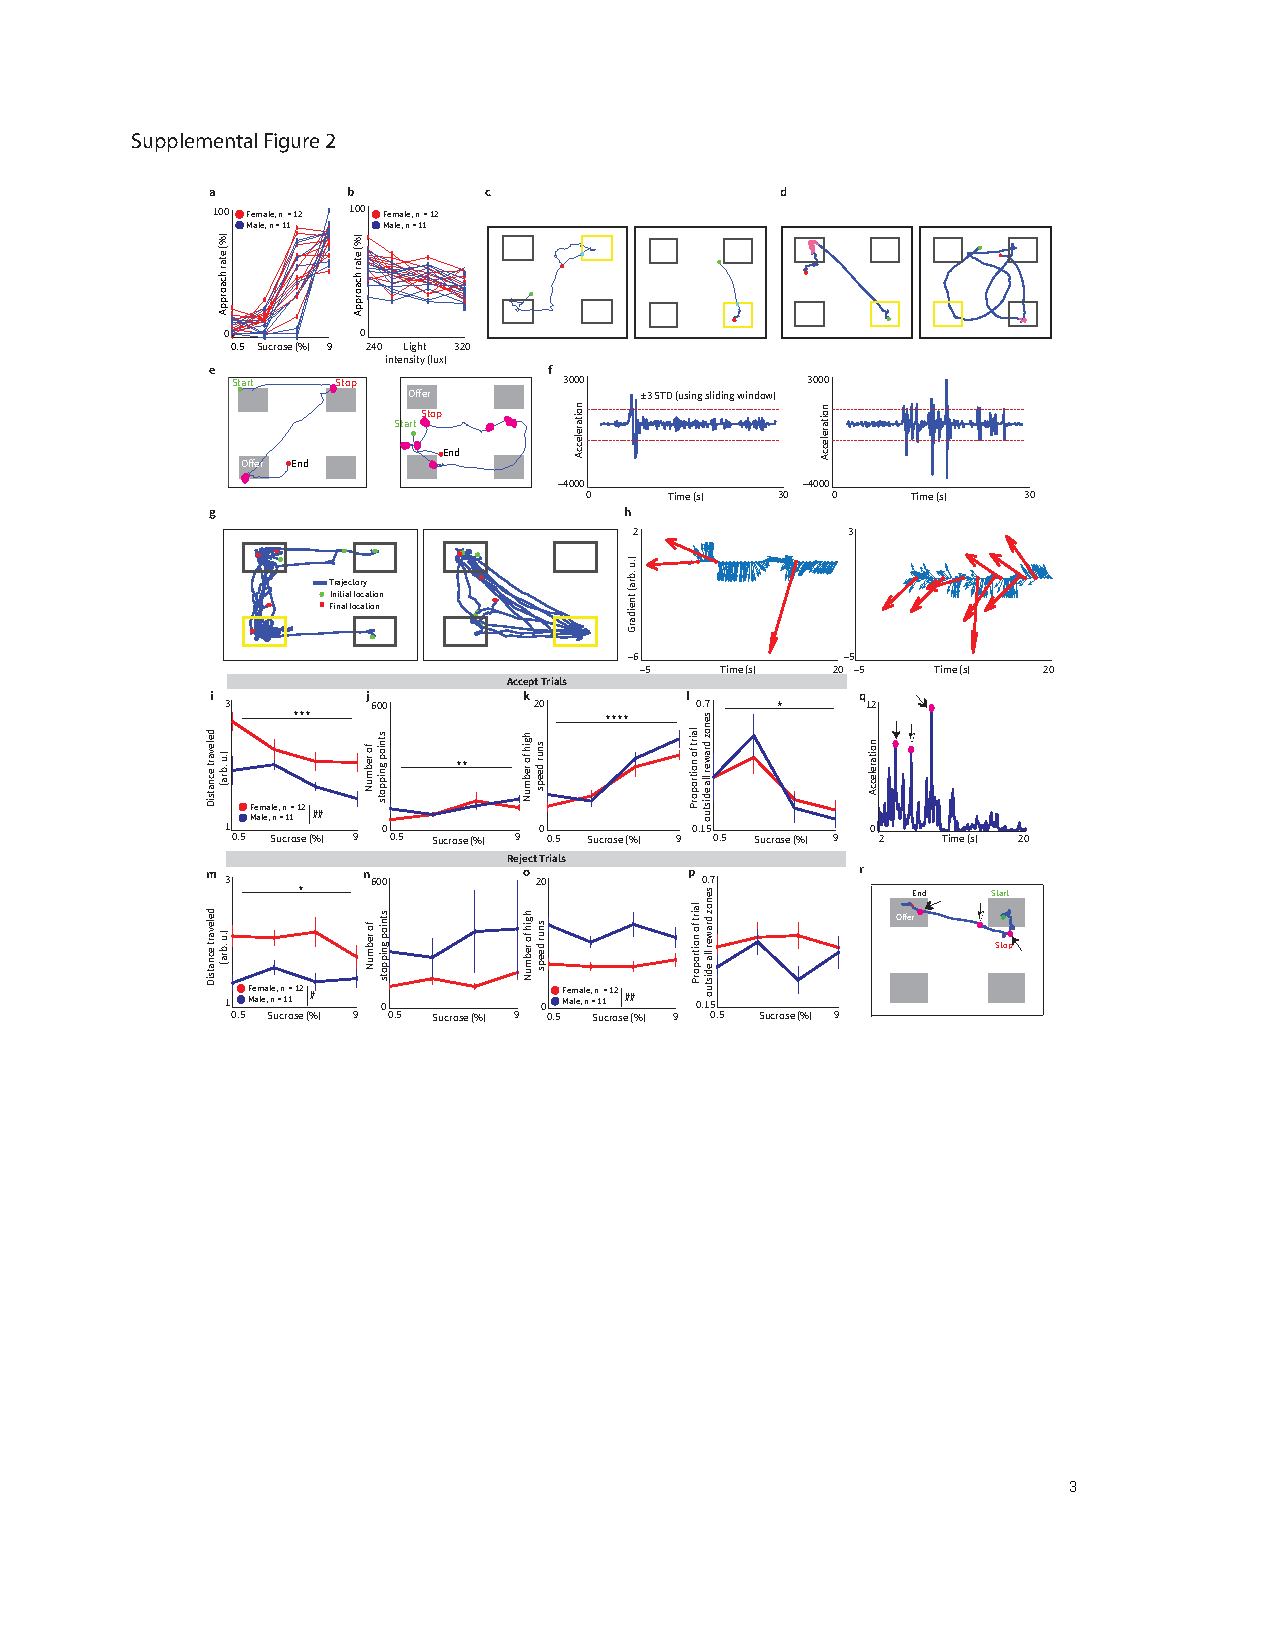
\includegraphics[width=\textwidth]{Figs/Record_SI_2.pdf}
\label{fig:Record_SI_2}
\end{suppfigure}

\clearpage

\begin{singlespace}
\noindent Figure S2. \textbf{Relevant decision-making features measured using rats’ timing of choice and spatial location during the task.} 
a. Approach rates across reward levels for individual rats. Error bars = mean ± SEM for all plots.
b. Approach rates across cost levels for individual rats.
c. Example trajectory when a low SC is offered (left) and when a high SC is offered (right, green
= trial start point, red = trial end point, pink = stopping points).
d. Trajectory examples tracked for two different rats during a trial. Some trajectories are direct
(left) while others are circuitous and indirect (right).)
e. We developed an algorithm that identifies when the rat does not move 0.1 units in the x or y
direction for 3 seconds (a \lq{stopping point}\rq) during a task.
f. We developed an algorithm that identifies high accelerations during individual rat trajectories.
High acceleration is identified by detecting speeds that are two standard deviations above the
mean (dotted line).
g. Multiple trajectories for a single rat on different trials are shown.
h. Rotation points (red arrows) are identified when the orientation of a rat’s body changes at least
180 degrees within 0.3 seconds.
i-l. Complementary to Fig. 2e-h, with analysis limited to trials in which the offers were approached
(excluding “reject” trials). Distance traveled during approach trials was impacted by both SC (i,
ANOVARM $***p = 0.00017$) and sex ($\#\# = 0.0038$). Number of stops during approach trials were
significantly affected by SC (j, $**p = 0.0015$) but not sex (p = 0.5). Frequency of high-speed runs
during approach trials was significantly affected by SC (k, $****p < 0.0001$) but not sex (p = 0.22).
Time outside feeder zones during approach trials was also affected by SC (l, $***p = 0.0003$) but
not sex (p = 0.9).
m-p. Limiting the analysis to trials in which the offers were rejected (not approached), number of
high-speed runs ($\#\#p = 0.0022$) and distance traveled ($\#p = 0.014$) were significantly different
between sexes. Distance traveled also decreased as concentration increased during reject only
trials ($*p = 0.047$). Number of stopping points (p = 0.22) and proportion of trial outside all reward
zones (p = 0.3) had no significant sex or concentration interactions (see Methods: Statistics and Reproducibility for all statistics). q-r. Example of direct relation between acceleration (r) and animal location (s) where stopping
points are temporally localized. This shows that RECORD has sufficient temporal resolution to provide precise 
timestamps that can be related across “features”. Arrows indicate sharp increase in acceleration (left) that 
correspond to movement initiation (right).
\end{singlespace}

\clearpage

\begin{suppfigure} 
\centering
  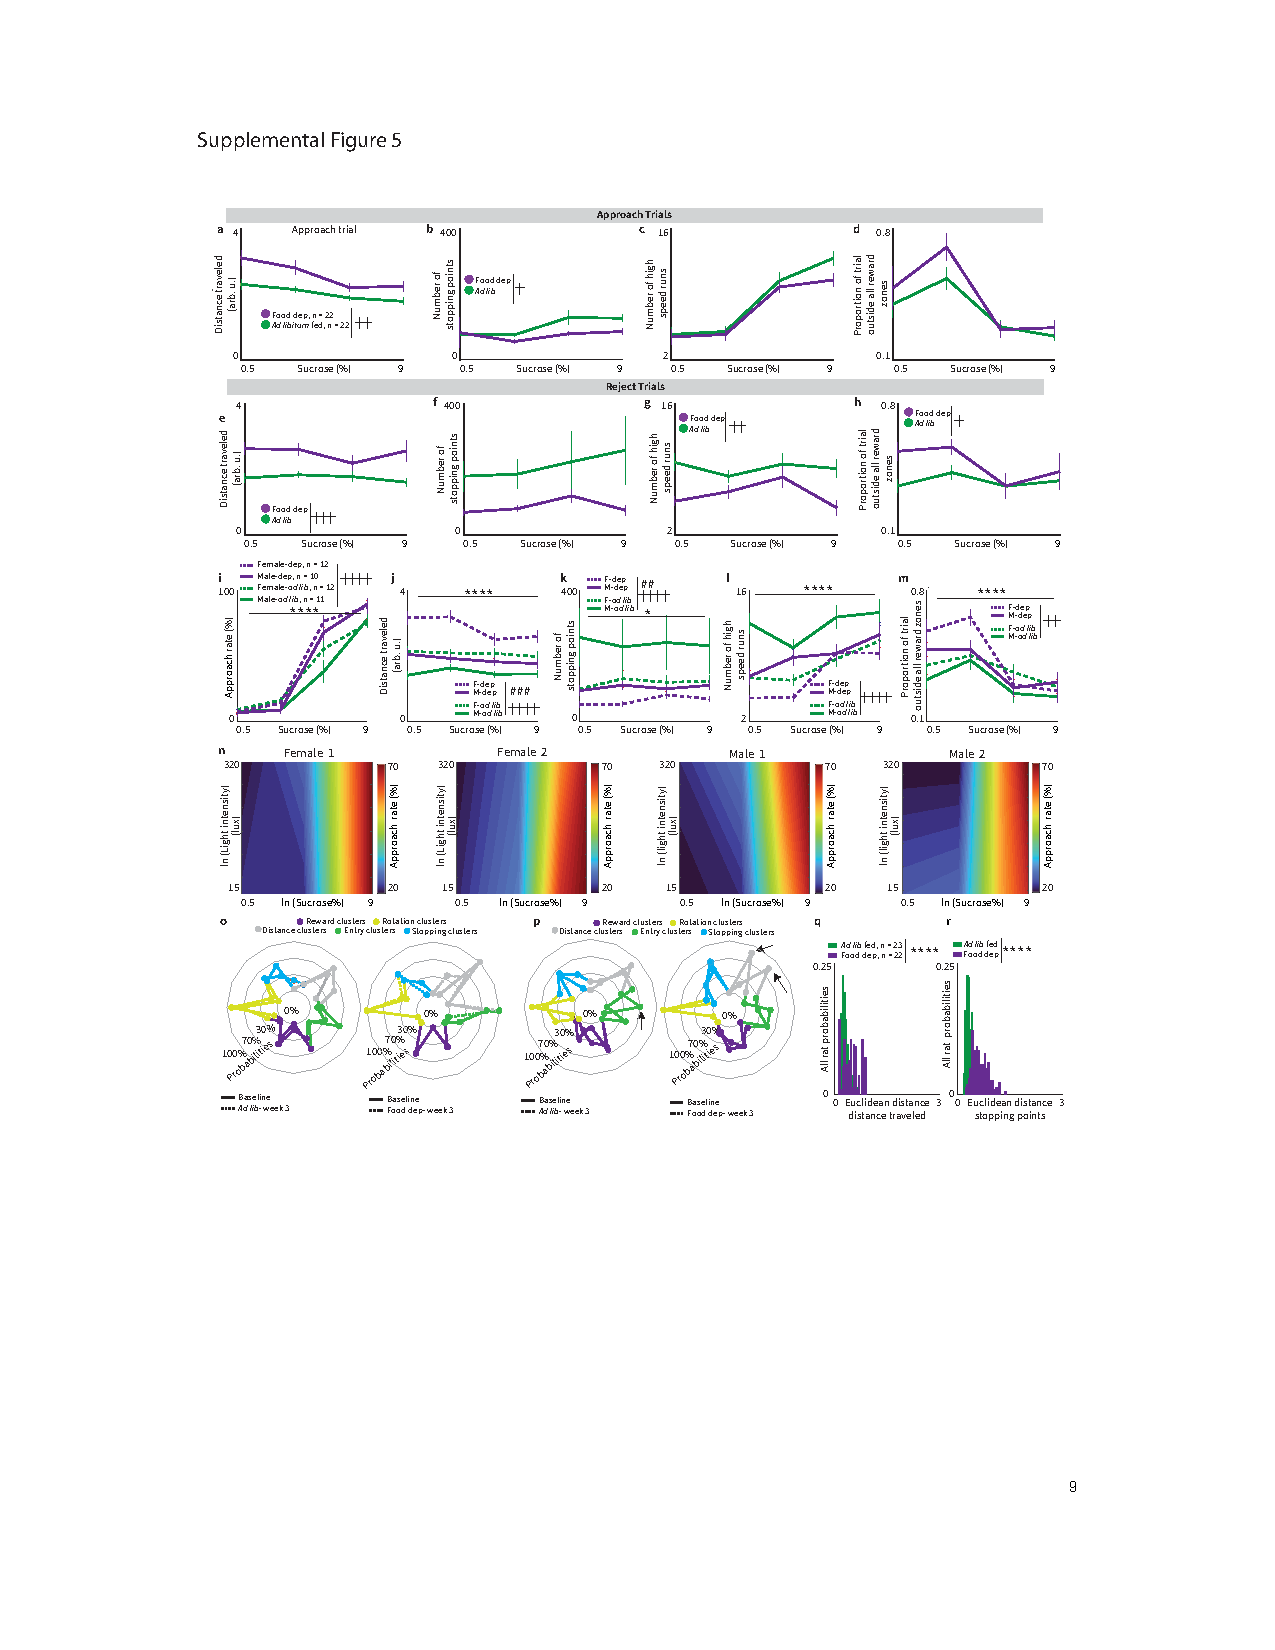
\includegraphics[width=\textwidth]{Figs/Record_SI_3.pdf}
  \label{fig:Record_SI_3}
\end{suppfigure}

\clearpage

\begin{singlespace}
    \noindent Figure S3. \textbf{Additional food deprivation data} a-d. During approach-only trials, the distance traveled was significantly greater during food deprived sessions (main effect of deprivation, ++p = 0.0033) while the number of stopping points
decreased in sessions conducted under food deprivation (main effect of deprivation, $+p = 0.021$).
In contrast, deprivation did not impact the number of high-speed runs (p = 0.4263) or proportion
of trial spent outside all reward zones (p = 0.08). Error bars = mean ± SEM for all plots.
e-h. During reject-only trials, the distance traveled was significantly greater during sessions
conducted under food deprivation (main effect of deprivation, $+++p = 0.0002$), while the number
of stopping points was unaffected (p = 0.14) However, the number of high-speed runs is
significantly lower under deprivation ($++p = 0.0034$) and proportion of the time spent outside all
reward zones is enhanced by deprivation (+p = 0.012).
i-m. Sex differences in behavioral features are still present during food deprivation, however these
sex differences shift. Approach rate, number of acceleration points, and time outside feeder have
similar patterns of significance before and during food deprivation. Distance traveled had
concentration become significant (ANOVARM $****p < 0.0001$) while sex remained significant (\#\#\#p
= 0.0002). Number of stopping points had significant differences between both concentration
(ANOVARM *p = 0.01) and sex (ANOVARM $\#\#p = 0.007$) compared to both concentration and sex
being insignificant before food deprivation. Figure 2 data was replotted for comparison as dashed
lines. When comparing across sex, sucrose concentration, and food deprivation vs. ad libitum fed
every feature was significantly different across food deprivation (main effect of condition,
approach rate: $++++p < 0.0001$, distance traveled: $++++p < 0.0001$, number of stopping points:
$++++p < 0.0001$, number of high-speed runs: $++++p < 0.0001$, and proportion of trial outside all
reward zones: $++p = 0.0026$).
n. Examples of individual cost-benefit maps from four different food-deprived rodents (2 females,
left, and 2 males, right).
o-p. Food deprivation impacts the clustering of behavioral features. Radar plot showing the cluster
distribution compared between ad libitum fed and food-deprived conditions. Two examples with
small changes in Euclidean distance (o) and changes in Euclidean distance (p). Arrows indicate
clusters of behavioral features that display the greatest changes between conditions.
q-r. Using the average cluster distribution of ad libitum fed rats, we created a distribution. We then
calculated the Euclidean distance of each cluster of distance between ad libitum fed and food
deprivation conditions for both distance traveled (q) and stopping points (r)and found that food
deprivation shifted the peak completely outside of the baseline normal distribution. These shifts
were statistically significant for both groups ($****p < 0.0001$, determined by two-sample
Kolmogorov-Smirnov test).
\end{singlespace}

\clearpage

\begin{suppfigure} 
\centering
  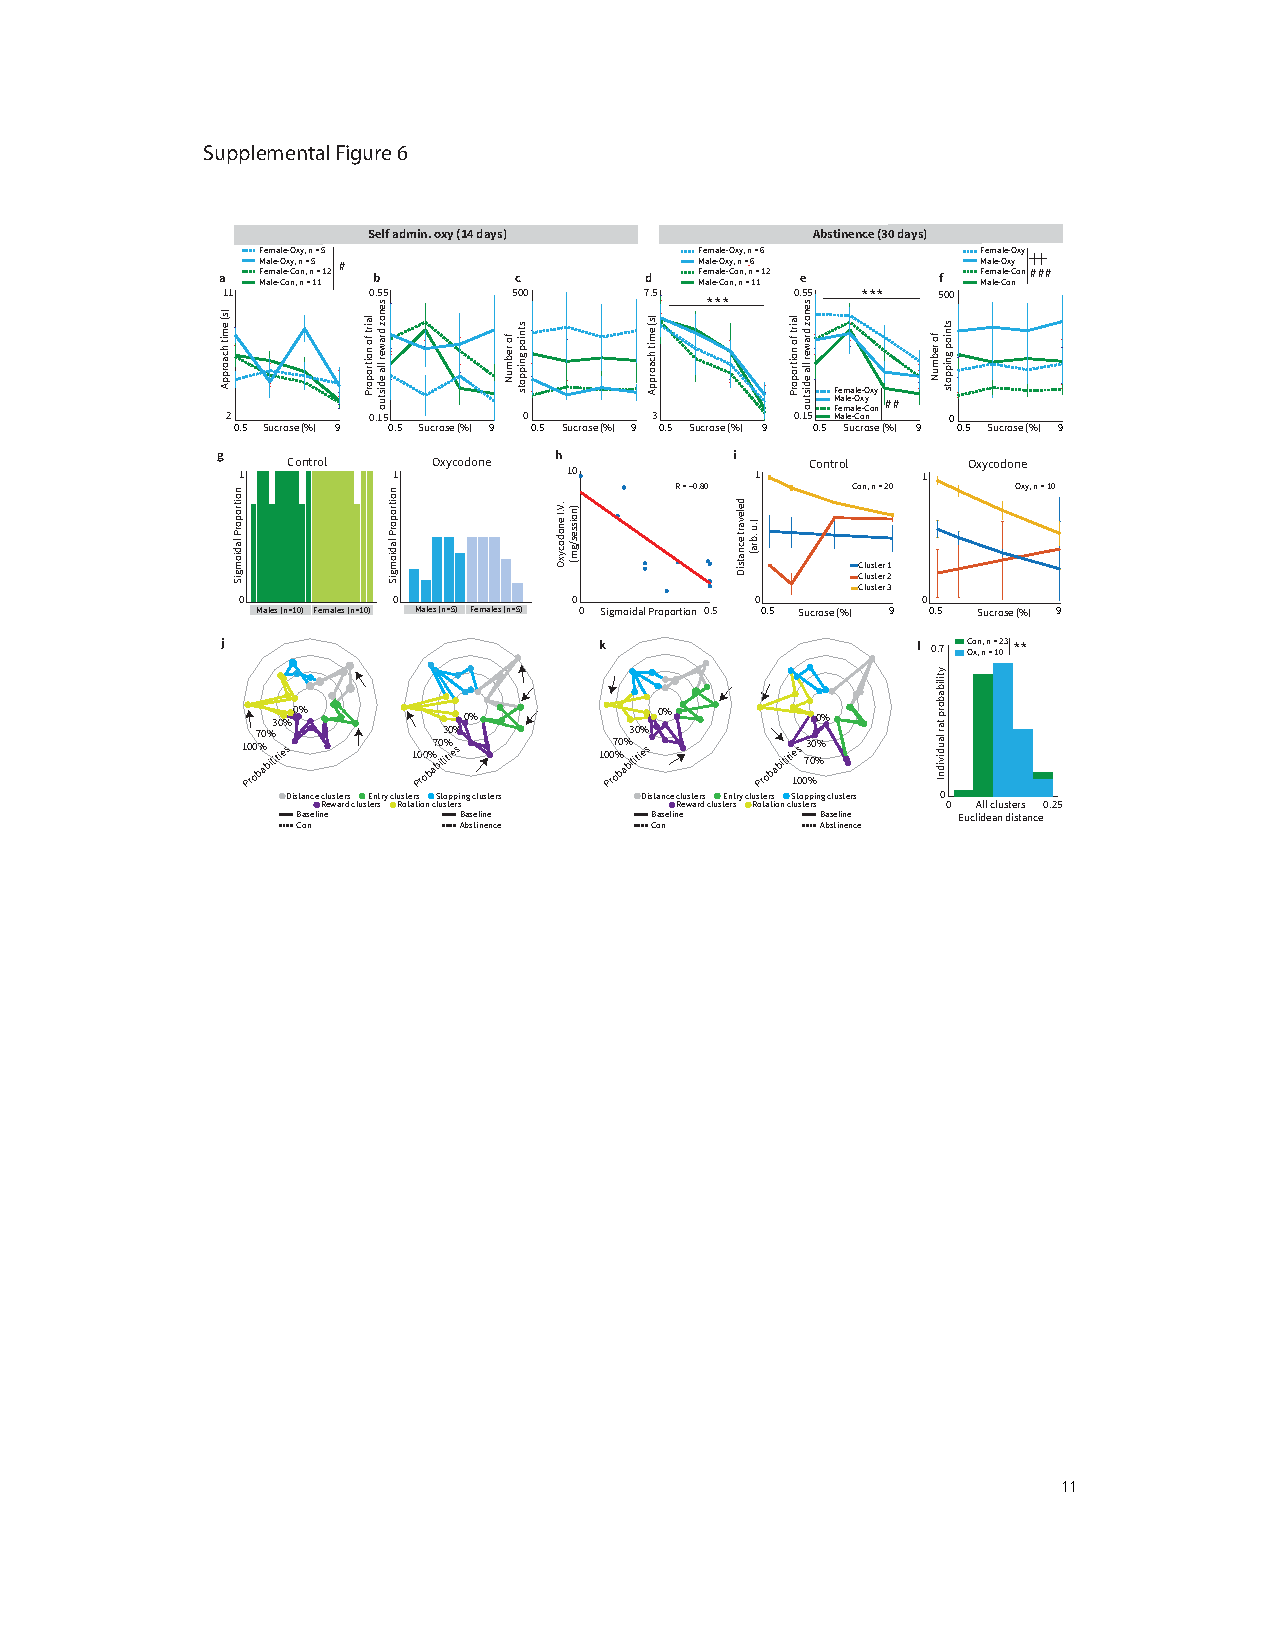
\includegraphics[width=\textwidth]{Figs/Record_SI_4.pdf}
  \label{fig:Record_SI_4}
\end{suppfigure}

\clearpage

\begin{singlespace}
    \noindent Figure S4. \textbf{Additional Oxycodone data.} a-c. (a) Approach time during self-administration task performance was significantly different
between sexes (effect of sex \#p = 0.0315), primarily due to the spikes seen in males at 0.5\% and
5\% sucrose concentrations, whereas concentration had no significant effects. No significant
differences were found when analyzing interactions between sex, concentration, and condition
(n-way ANOVArm, sex x condition, sex x concentration, and condition x concentration). Error bars
= mean ± SEM for all plots. (b) Proportion of trials outside feeder zone had no significant
interactions between concentration or sex. No significant factors were observed across control
and self-administration while the only significant interaction detected was between sex and
condition (p = 0.0005, n-way ANOVArm). (c) The number of stopping points similarly had no
significant effects of concentration or sex. When compared to the control group there were no
significant main effects while there was a significant interaction between sex and condition (p <
0.0001, n-way ANOVArm).
d-f. After oxycodone, features seem to trend towards pre-oxycodone shapes. (d) The effect of
sucrose concentration went from not being significant during oxy self-administration to becoming
significant again (***p = 0.0003, n-way ANOVArm), with no significant interactions between the
control group and abstinence conditions. (e) The proportion of the trial spent outside all feeder
zones decreased as sucrose concentration increased with no significant interactions detected
between conditions, meanwhile the main effect of sex (p = 0.0063) and concentration (***p =
0.0006, n-way ANOVArm) became significant between baseline and abstinence groups. (f) When
comparing abstinence groups, the number of stopping points remained insignificant across
concentration and sex. However, when compared to the control group there were significant main
effects of sex (\#\#\#p = 0.0005) and condition (++p = 0.006, n-way ANOVArm) with no significant
interactions between sex, condition, or concentration.
g. Individual sigmoid frequencies across control and oxycodone conditions.
h. Correlation plot between amount of oxycodone self-administered and sigmoid frequency. We
were unable to track the opioid self-administration of one rat due to technical difficulties.
i. Average psychometric functions extracted from distance traveled clusters between control (left)
and oxycodone (right) conditions.
j,k. Oxycodone impacts the clustering of behavioral features. Radar plot showing the cluster
distribution compared between baseline and oxycodone conditions. Some rats have small
changes in Euclidean distance (j) or large changes (k). Arrow indicates a feature that has
shifted.
l. Individual Euclidian distances between clusters for baseline and oxycodone self-administration
conditions (**p = 0.0011, two-sample Kolmogorov-Smirnov test).
\end{singlespace}

\clearpage

\section{Future Work}
\noindent\textbf{Integrating Advanced Behavioral Analysis with DeepLabCut and A-SOiD}\\
While the current thesis has provided significant insights into the decision-making processes of rodents under acute alcohol consumption and through the use of the RECORD system, there remains substantial room to deepen our understanding of behavior through the use of advanced computational tools. In particular, utilizing DeepLabCut and A-SOiD offers exciting possibilities for quantifying complex behaviors that are difficult to capture with traditional methods. These tools can enhance the resolution and granularity of behavioral analysis, particularly in understanding motor patterns, micro-movements, and social interactions that may influence decision-making.

\begin{enumerate}
    \item \textbf{Behavioral Analysis with DeepLabCut}\\
    DeepLabCut is a markerless pose estimation tool that has revolutionized the field of animal behavior research. This tool allows for the accurate tracking of body parts during behavior without the need for physical markers, making it ideal for studying naturalistic and unencumbered behavior in rodent models.
    
    \begin{enumerate}
    \item \textbf{Enhancing Decision-Making Analysis}\\
    Currently, the RECORD system provides a high-level overview of decision-making behavior through task performance metrics, such as the number of choices, approach/avoidance behavior, and latency to choose. However, these metrics do not capture the nuances of how physical actions (e.g., approach trajectories, head movements, paw placements) may correlate with decision-making under conditions of alcohol consumption.

    \vspace{1em}

    By integrating DeepLabCut, future research can explore the detailed motor sequences that underlie decision-making processes. For instance, the system could track body parts such as the head, limbs, and tail to determine how a rat’s approach to different corners of the test arena evolves over time, especially when alcohol is introduced. This data could be compared between male and female rats to see whether sex-dependent differences are also reflected in movement dynamics, providing deeper insight into how alcohol alters not just decision-making but motor execution of choices.
    
    \item \textbf{Alcohol-Induced Changes in Movement Patterns}\\
    DeepLabCut could also be used to investigate whether alcohol consumption leads to more subtle, alcohol-induced changes in gait or posture. For instance, alcohol may impair fine motor control, leading to more erratic or slowed movements during the decision-making process. By quantifying these changes, it would be possible to determine whether males and females differ in their physical response to alcohol and how these changes relate to decision outcomes. This could shed light on whether impaired motor control influences poor decision-making or if decision-making alterations occur independently of motor function.
    \end{enumerate}

    \item \textbf{Social Behavior and A-SOiD for Behavioral Classification}\\
    A-SOiD (Automated Social Investigation Detector) is a powerful tool for classifying social behaviors, including aggressive and investigative actions, using machine learning. While the current work has focused on individual decision-making, alcohol consumption is known to affect social behavior in both humans and animals. Exploring social dynamics during decision-making tasks could provide valuable insight into how alcohol affects not just individual behavior but interactions between subjects.

    \begin{enumerate}
        \item \textbf{Investigating Social Influence in Decision-Making}\\
        Future studies could involve adding a social component to the RECORD system by including a second rat in the testing arena, and A-SOiD could be employed to classify behaviors such as social investigation, dominance, or avoidance. Alcohol might enhance or diminish social interactions, influencing decision-making indirectly. For instance, a rat’s willingness to approach a particular alcohol/sucrose concentration could be affected by the presence of another rat displaying either approach or avoidance behavior. Using A-SOiD, we can capture detailed behavioral exchanges and categorize them, allowing for an exploration of how social contexts modulate decision-making under the influence of alcohol.

        \item \textbf{Social Aggression and Avoidance}\\
        The sex-dependent differences in alcohol-induced decision-making identified in this thesis may also extend to social behavior. A-SOiD could be used to track aggression or avoidance behaviors that may arise under alcohol exposure, particularly in competitive situations where multiple rats are presented with the same choice options. For example, alcohol might heighten aggression in males, leading to increased competition for high-sucrose, low-alcohol options, while females may exhibit less social conflict. Analyzing these dynamics would offer insight into the broader social consequences of alcohol consumption.

    \end{enumerate}

    \item \textbf{Machine Learning for Behavioral Phenotyping}\\
    Combining data from DeepLabCut and A-SOiD will generate a rich set of features, including both fine-grained motor behaviors and social interaction patterns. This data can be leveraged with machine learning techniques to develop comprehensive behavioral phenotypes of decision-making under alcohol exposure.
    
    \begin{enumerate}
        \item \textbf{Clustering Behavioral Phenotypes}\\
        By using unsupervised machine learning techniques such as k-means clustering or Gaussian mixture models, we can identify distinct behavioral phenotypes that correspond to different decision-making strategies. For example, some rats may exhibit more cautious, avoidance-driven behavior, while others may be more risk-seeking. These phenotypes may vary depending on alcohol consumption and could provide a more nuanced understanding of how alcohol affects decision-making on a spectrum, rather than simply categorizing rats into broad groups based on sex.

        \item \textbf{Predicting Vulnerability to Alcohol Use Disorder}\\
        One of the key goals of the current work is to develop methods for identifying individuals at risk for alcohol use disorders (AUD). Using machine learning models trained on behavioral data from DeepLabCut and A-SOiD, we could predict which subjects are more likely to engage in irrational decision-making under the influence of alcohol. This could involve identifying predictive features, such as particular movement patterns, approach trajectories, or social behaviors, that signal an increased risk for AUD. Ultimately, these models could be applied to future experiments as screening tools for early identification of vulnerable populations.

    \end{enumerate}

    \item \textbf{Cross-Species Translational Potential}\\
    One of the advantages of tools like DeepLabCut and A-SOiD is that they can be easily adapted to study decision-making in other species, including humans. By applying these same computational tools in translational studies, we could directly compare rodent decision-making under alcohol exposure to human decision-making patterns, enhancing the translational relevance of the research.

    \begin{enumerate}
        \item \textbf{Adapting to Human Studies}\\
        While the current research is focused on rodents, many of the behavioral patterns identified using DeepLabCut and A-SOiD could be translated to human studies. For instance, motion tracking and classification tools could be adapted for use in human subjects performing decision-making tasks in a virtual environment. These cross-species comparisons could provide deeper insights into the conserved neural mechanisms underlying alcohol-induced decision-making impairments and aid in developing therapeutic interventions for AUD.
    \end{enumerate}
    
\end{enumerate}

\begin{center}
\begin{tabular}{ |c|c| } 
 \hline
 Date & Tasks to complete \\
 \hline
 Oct - Nov 2024 & Train and evaluate a neural network on training dataset with DeepLabCut\\
 Dec 2024 & Extract feature and analyze novel videos with A-SOiD\\
 Jan - Feb 2025 & Writing manuscript\\
 Mar - Apr 2025 & Manuscript revision and submission\\
 May 2025 & Thesis writing: Literature review and Methodology\\
 Jun 2025 & Thesis writing: Experiment and Results\\
 Jul - Aug 2025 & First draft\\
 Sep - Oct 2025 & Defense\\
 \hline
\end{tabular}
\end{center}

\clearpage


\section{References}
\bibliographystyle{plain}
\bibliography{ref.bib}

\clearpage

\section{Curriculum Vita}

\end{document}
